\documentclass[notes]{beamer}
%\documentclass{beamer}
\usepackage{beamerthemesplit}

%\usetheme{Warsaw} % Beamer theme v 3.0
%\usecolortheme{default} % Beamer color theme
%\setbeamercolor{frametitle}{fg=blue,bg=white}

\beamersetuncovermixins{\opaqueness<1->{25}}{\opaqueness<2->{15}}
%%\setbeamertemplate{itemize item}[*]
%\setbeamertemplate{itemize items}[triangle]
%\setbeamertemplate{enumerate item}{(\insertenumlabel)}

\usecolortheme[named=blue]{structure}
\mode<presentation>
{
  \usetheme{Warsaw}
  \setbeamercovered{transparent}
  \setbeamertemplate{items}[ball]
  \setbeamertemplate{itemize items}[triangle]
  \setbeamertemplate{enumerate item}{(\insertenumlabel)}
  \setbeamertemplate{theorems}[numbered]
  \setbeamertemplate{footline}[frame number]
}

\setbeamertemplate{navigation symbols}{}



%bibliography styles
\usepackage{natbib}
% fix natbib-beamer problem
\def\newblock{}

% TIPA
\usepackage{tipa}
% multicolumns
\usepackage{multicol}
% href
\usepackage{hyperref}
% subfigure
\usepackage{subcaption}
% table multicol and multirow
\usepackage{multicol}
\usepackage{multirow}


% Rotating Objects and Captions
\usepackage{hvfloat}
%%% Lingua 
%\usepackage[brazil]{babel}
%%% acentua<E7><E3>o
\usepackage[utf8]{inputenc}

% animation
\usepackage{animate}





\title{Patterns in Language Usage}
\author[Leonardo Araujo]{Leonardo Araujo \\ \footnotesize supervisors: Hani Yehia and Tha\"{i}s Crist\'{o}faro-Silva\\ UFMG}
\date{\today}

\begin{document}

\frame{\titlepage}



%\AtBeginSection[]
%{
%  \begin{frame}<beamer>[allowframebreaks]
%  \begin{footnotesize}
%    \frametitle{Outline}
%    \tableofcontents[current,currentsection]
%  \end{footnotesize}
%  \end{frame}
%}

\AtBeginSection{
    \begin{frame}[noframenumbering]
        \frametitle{Outline}
        \tableofcontents[currentsection,hideothersubsections]
    \end{frame}
}


%\section[Outline]{}
\frame[allowframebreaks]{\begin{footnotesize}\tableofcontents\end{footnotesize}}



\section{Introduction}

\subsection{Language}
\frame
{
  \frametitle{Language}
  %\begin{columns}[c] % the "c" option specifies center vertical alignment
  %  \column{.6\textwidth} % column designated by a command
       \begin{block}{language: system of communication}
        Language is a complex system that uses signs to encode and decode information to convey communication.
       \end{block}      
      
       \vspace{0.5cm} 
       Language must be statable in a finite form \citep{donalddavidson,humboldt1836,chomsky1969,mandelbrot,wang1991}. 
       
  %
  %  \column{.4\textwidth}
  %     \begin{figure}[h!]
  %     \centering
  %     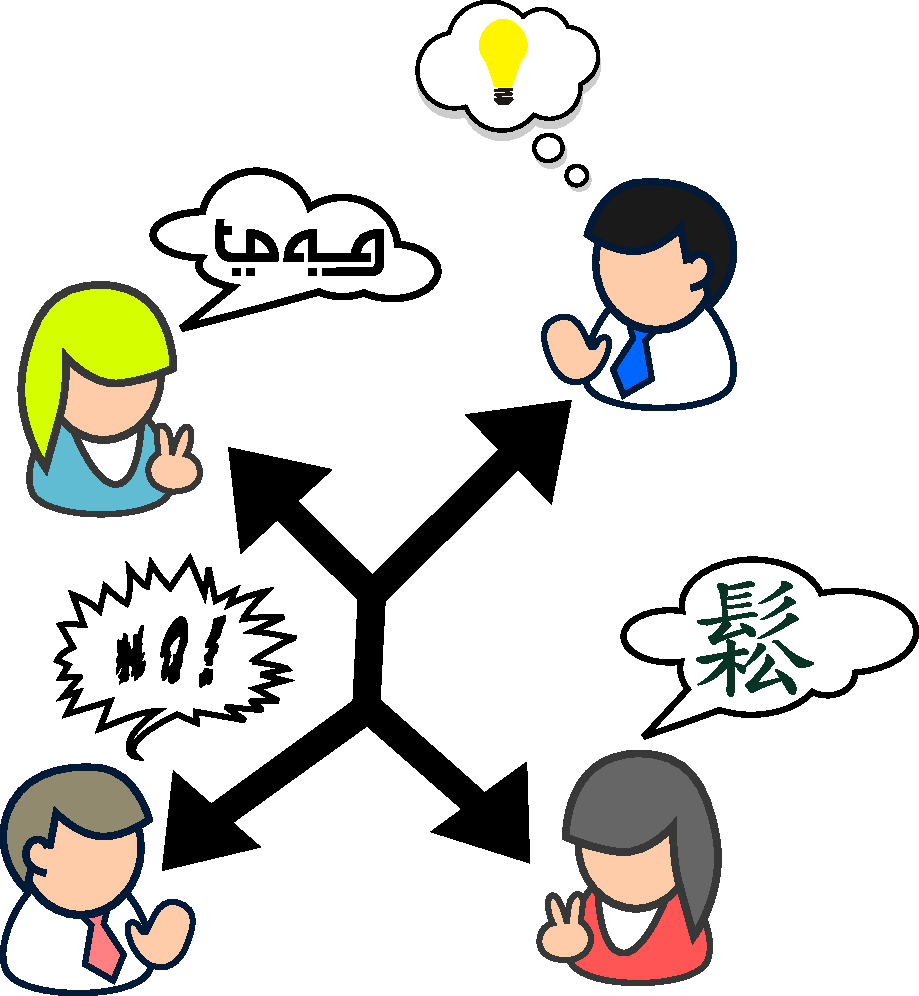
\includegraphics[width=0.9\textwidth]{imagespresentation/communication.pdf}
  %     \caption{Language.}
  %     \label{fig:communication}
  %     \end{figure}
  %
  %\end{columns}
}
\note{
Language is a human capacity for acquiring and using complex systems of communication.
A language in this sense is a system of signs for encoding and decoding information.
Language is a social process of human iteration, an then it is made possible by our biological capabilities (and so limited by its biological restrictions) and shaped by our psychological aspects.


Language has a fundamentally social function. Processes of human interaction 
along with domain-general cognitive processes shape the structure and knowledge of 
language.
}
\note{
``Along with its social function, language is importat to humans as a mental instrument.
Indeed, the invention of language -- that is, the accumulation of symbols to represent emotions,
objects, and acts -- may be the most important event in human evolution, because so many developments
follow from it''\citep{wang1996}.
}
\note{
Recent research across a variety of disciplines in the cognitive sciences has 
demonstrated that patterns of use strongly affect how language is acquired, is structured, 
is organized in cognition, and changes over time.

However, there is mounting evidence 
that processes of language acquisition, use and change are not independent from one 
another but are facets of the same system.
}
\note{
Is there Thought without Language?

``Thoughts are forms conceived in the mind, rather than the forms perceived through the five senses. Thought and thinking are the processes by which these concepts are perceived and manipulated. Thinking allows beings to model the world and to represent it according to their objectives, plans, ends and desires.''.
}
\note{
In 1967 Donald Davidson (philosopher) published ``Truth and Meaning'', in which he argued that any learnable language must be statable in a finite form, even if it is capable of a theoretically infinite number of expressions -- as we may assume that natural human languages are, at least in principle. If it could not be stated in a finite way then it could not be learned through a finite, empirical method such as the way humans learn their languages.


We are finite beings whose mastery of the indefinitely many
expressions of our language must somehow arise out of our mastery of finite
resources. Otherwise, there would be an unbounded number of distinct
things to learn in learning a language, which would make language learning
impossible for finite beings like ourselves. The linguistic competence of a
finite being of our sort must be the result of the interaction of a finite number
of basic competencies.
}
\note{
Ever since Humboldt (1836/1999), researchers have hypothesized that language makes 
``infinite use of finite means.'' Yet the study of language had to wait nearly a century 
before the technical devices for adequately expressing the unboundedness of language became 
available through the development of recursion theory in the foundations of mathematics 
(cf. Chomsky, 1965). Recursion has subsequently become a fundamental property of grammar, 
permitting a finite set of rules and principles to process and produce an infinite number of expressions.

\vspace{0.3cm}
``Segmental phonology and hierarchic syntax are of partcular importance''\cite{wang1991}.
}
\note{
Apostel's article: ``Logique et langage consid\'{e}r\'{e}s du point de vue de la pr\'{e}correction des erreurs''.
Trubetskoy attempted to characterize phonemic systems as maximally 'coherent' the more they 
consist of 'bilateral,homogeneous, privative, proportional, and neutralizable' oppositions.
We might understand as a branching-diagrams of phonemic oppositions which is characterized by
the binarity of the nodes, symmetry of the branches, and parsimony in the use of phonetic features.
Thus, to require a `coherent' system to contain `privative' oppositions, as opposed to
`gradual' and `equipollent' ones (which is to say that each pair of opposed
phonemes must share at least one feature and differ in at least one feature,
while no more than two phonemes which share some set of features can differ
by any one feature), is simply to require that all nodes, or branching-points,
in the branching-diagram of the phonemes by their phonetic features be binary.
}
\note{
Similarly, requiring oppositions to be `proportional' rather than `isolated', i.e.
requiring that there be more than one opposition for which the opposed phonemes
differ by some given set of features, is simply to reduce the number of different
features used for a given number of oppositions and thus to increase economy,
or parsimony.
}
\note{
Apostel then goes on to show that such constraints on the kind of oppositions
allowed in a `coherent' phonological system are exactly analogous to the constraints 
which one would impose upon an error-correcting code for optimality of coding and error-correction.
Briefly, an error-correcting code is one in which
redundancy has been introduced by the addition to certain message units of
extra symbols so chosen that a random, noise-produced alteration in one or more
message symbols will result in a detectable change in some prearranged arithmetic 
or logical function and thus permit the detection and correction of the error. 
}
\note{
One scheme for detecting one error per word would require each code word
to differ from every other code word by at least two letters, for an alteration of
one letter in any word would render that word different from all admissible code
words (but the error would not be correctable, for any given nonword received
might be an alteration of several code words). Now optimal coding requires
that these `distances' between code words be all equal, i.e. consist of the same
number of letter differences.
}
\note{
This and certain other simple requirements for optimality may now be interpreted 
as requirements of symmetry, binarity, and parsimony in a branching-diagram; 
for just as a code word is an ordered sequence of letter positions which
can take on only certain values (say 0 and 1), so a phoneme may be taken as an
ordered set of features each of which can take on only certain values (say + or -,
in the case of the binary choices admitted here). Thus, as far as symmetry of
the branching-diagram is concerned, code words in a simple Hamming error-detecting 
code are a model of phonemes considered as sets of phonetic features
under the requirement of coherence.
}
\note{
However, in order to generate most efficiently all the sentences of a language,
and to do this in such a manner as to segregate the optional phonemic rules
from the obligatory phonetic rules, and in such a manner as to represent properly
all the morphophonemic and phonemic facts known about sentences, it is necessary 
to build into the grammar of a language-indeed, into the phonological
part-a great deal more specificity of structure than is given by these relatively
superficial constraints of binarity, symmetry, and parsimony. In other words,
our coding model, though it may be mathematically correct, is compatible with
too many different possible grammars, for it does not reach to a deep enough level
of linguistic structure.

(Logique, langage et theorie de l'information reviewed by R. B. LEES)
}




\frame
{
  \frametitle{Language}

  \begin{columns}[c]
  
  \column{0.5\textwidth}  
  \begin{itemize}
  \item language unpredictable nature
  \item recurring patterns, language `universal'
  \item structures and organization
  \item the principle of least effort \citep{zipf1949} : fast and robust communication
  \item maximum entropy
  \end{itemize}
  
  \column{0.5\textwidth}
  \begin{figure}[h!]
  \centering
  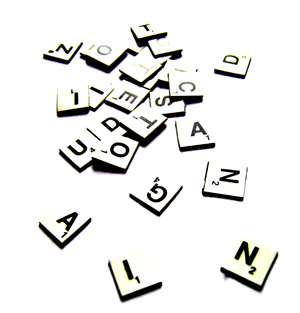
\includegraphics[width=0.95\textwidth]{images/scrabble.jpg}
  %\caption{Language unpredictable nature.}
  \label{fig:scrabble}
  \end{figure} 
 
  \end{columns}
}
\note{
Languages have unpredictable nature and without it there would be no communication at all. If it was a certain deterministic event, it would have no information associated.

The linguistic analysis of a language is the observation of certain recurring patterns.
Some patterns that are said to be frequently found in the languages of the world are
called `universal'.

To study and understand how languages works, it is important to find/define its structures and the way they are organized to build communication.

The idea proposed by \cite{zipf1949} is that language works seeking the principle of least
effort. The process of communication is better when it is possible to transmit information
in a fast and robust way.
}
\note{
The `linguistic universals' paradigm gives the impression that languages are 
all built to a common pattern. In fact, there are vanishingly few universals of language in the direct 
sense that all languages exhibit them. Instead, diversity can be found at almost every level of 
linguistic organization. This fundamentally changes the object of enquiry from a cognitive science 
perspective. 
}


\frame
{
  \frametitle{Language}
  Language is a complex adaptive system.  
  \begin{enumerate}
  \item multiple agents
  \item adaptive
  \item perception and motivation
  \item emergence of patterns
  \end{enumerate}
}
\note{
We argue that this system is best construed as a 
complex adaptive system (CAS). This system is radically different from the static system 
of grammatical principles characteristic of the widely held generativist approach. Instead, 
language as a complex adaptive system of dynamic usage and its experience involves the 
following key features: (1) The system consists of multiple agents (the speakers in the 
speech community) interacting with one another. (2) The system is adaptive, that is, 
speakers’ behavior is based on their past interactions, and current and past interactions 
together feed forward into future behavior. (3) A speaker’s behavior is the consequence 
of competing factors ranging from perceptual mechanics to social motivations. (4) The 
structures of language emerge from interrelated patterns of experience, social interaction, 
and cognitive processes.
}
\note{
Humans are great at statistical learning, which is the ability to track, sort and categorize 
sounds and visual patterns.

\vspace{0.5cm}
When it comes to learning either auditory or visual languages, infants are tracking the pattern of how words and parts of words come together. And by tracking the patterns, they can, based on the statistical regularities of which sounds came together, figure out what a word is, or where a word begins and ends. From this, their brains can form sound categories for their native language, which will cue them to pay more attention to those sounds in the future.
}

\frame
{
  \frametitle{Language}
  \begin{figure}[h!]
  \centering
  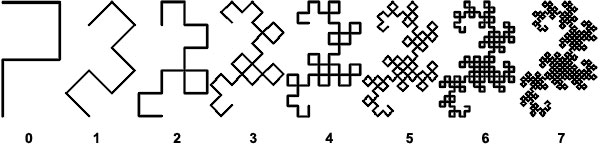
\includegraphics[width=0.6\textwidth]{imagespresentation/dragon.png}
  \caption{Dragon fractal.}
  \label{fig:dragon}
  \end{figure} 
  \begin{figure}[h!]
  \centering
  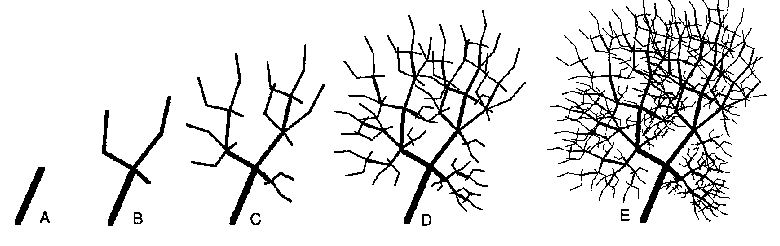
\includegraphics[width=0.6\textwidth]{imagespresentation/purkinje.png}
  \caption{Purkinje cell, fractal model.}
  \label{fig:purkinje}
  \end{figure}
}
\note{
Our assumption is that the complex patterns and rules observed in language communication are emergent from
the multiple interactions of speech agents over time. We believe there are simple fundamental laws
that rule a multitude of microscopic interactions which create the observed macroscopic properties
apparently complex. We believe language presents a fractal nature.
}




\subsection{Quantitative Linguistics}
\frame
{
  \frametitle{Quantitative Approach}
  \begin{itemize}
  \item systematic empirical investigation of phenomena via statistical, mathematical or computational techniques
  \item develop and employ mathematical models, theories and/or hypotheses pertaining to the phenomena
  \item measurement: empirical observation 
  \end{itemize}
}
\note{
An immense number of properties and processes in language which can be detected and analysed only with quantitative methods on the basis of quantitative concepts: features and interrelations which can be expressed only by numbers or rankings

\vspace{0.5cm}
It can be shown that these properties of linguistic elements and their interreations abide by universal laws, which can be formulated in a strict mathematical way - in analogy to the laws of the well-known natural sciences.
 Emphasis has to be put on the fact that these laws are stochastic; they do not capture single cases (this would neither be expected nor possible), they rather predict the probabilities of certain events or certain conditions in a whole. 

\vspace{0.5cm}
\scriptsize{abide: accept or act in accordance with (a rule, decision, or recommendation)}
}
\note{
A law can be said to be a statement representing universal patterns in the world (the phenomenological type of law) or universal mechanisms (the representational or mechanistic type).


\vspace{1cm}
 types of laws:
 1) probability distributions, i.e. it makes predictions about the number of units of a given property - Zipf-Mandelbrot Law
 2) functional type, because these laws link two (or more) variables, i.e. properties - Menzerath’s Law, which relates the size of linguistic constituents to the size of the corresponding construct
 3) developmental type - a property is related to time - Piotrowski Law, which represents the development (increase and/or decrease) of the portion of new units or forms over time.
}

\frame[allowframebreaks]
{
  \frametitle{Quantitative Linguistics - History}
  \begin{itemize}
  \item date back in the ancient Greek - applications of combinatorics 
  \item 718-791, philologist and lexicographer Al-Khalil ibn Ahmad - permutations and combinations to list all possible Arabic words with and without vowels
  \item 1564-1614, William Bathe - \emph{Janua Linguarum}, the world's first language teaching texts, where he had compiled a list with 5.300 essential words
  \item the first scientific counts of units of language or text were published already in the 19th century as a means of linguistic description - in Germany, Förstemann (1846, 1852) and Drobisch (1866), in Russia, Bunjakovskij (1847), in France Bourdon (1892), in Italy, Mariotti (1880), in England, Augustus De Morgan (1851) and in the USA, probably Sherman (1888)
  \item the Russian mathematician Andrey Andreyevich Markov who created the base of the theory of Markov chains in 1913
  \item George Kingley Zipf was the first to set up a theoretical model in order to explain the observations and to find a mathematical formula for the corresponding function - the famous ``Zipf’s Law'' (1935, 1949)
  \item Benoît Mandelbrot (1953, 1959, 1961a, 1961b)
  \item Shannon and Weaver (1949) - Information Theory
  \item Gustav Herdan (1954, 1956, 1960, 1962, 1964 1966, 1969), Rajmund.G. Piotrowski (1959, 1968, 1979) and Walter Meyer-Eppler (1959)
  \item today, Quantitative Linguistics is a well-developed scientific discipline with a broad applicational impact
  \end{itemize}

}

\frame
{
  \frametitle{Laws in Quantitative Linguistics}
  \begin{itemize}
  \item Zipf-Mandelbrot - frequency and rank are inversely related
  \item Menzerath - the size of linguistic constituents decreases as the size of the corresponding construct increases
  \item Heaps (Herdan) - relation between lexical size and text size
  \item Piotrowski - development of new units or forms over time
  \end{itemize}
  
  \begin{small}
  Laws in Quantitative Linguistics (Universit\"{a}t Trier)
  \href{http://lql.uni-trier.de}{http://lql.uni-trier.de}

  Glottopedia
  \href{http://www.glottopedia.org/}{http://www.glottopedia.org/}
  \end{small}
}
\note{
The Piotrowski's law states over the language change, proposing a mathematical model to it and delimiting 
which path could changes produce. The basic idea is that the change comes from the realization of
one pearson and that may produces a gradual spread. The greater the number of people that takes on this change,
the faster will be the spreading process.

\vspace{0.5cm}
This idea seems in accordance with the `lexical diffusion' proposed by Wang.
}


\subsection{Structuralism}

\frame
{
  \frametitle{Structuralism}
  
  Structural linguistics
  \begin{itemize}
  \item Ferdinand de Saussure - \textit{Course in General Linguistics} in 1916.
  \item theoretical paradigm: elements must be understood in terms of their relationship to a larger, overarching system or structure
  \item linguistic signs were composed of two parts: \emph{signifier} and \emph{signified}
  \item linguistic levels: the phonemes, morphemes, lexical categories, noun phrases, verb phrases, and sentence types 
  \end{itemize}
  
  \vspace{0.5cm}
``En matière de langue on s’est toujours contenté d’opérer sur des unités mal définies''\footnote{In language's matter it has always been sufficient to operate on ill-defined units.} \citep{saussure}.

}
\note{
The structuralism brings a new paradigm where we understand language as system where elements stablish relations
one to another and to a larger structure creating the whole.

\vspace{0.5cm}
It creates a dissociation of the signifier and signified and brings the linguistic analysis to multiple levels.

\vspace{0.5cm}
In order to stablish a logical interpretation and understanding of language, it is necessary to 
do so by establishing linguistic units that my be used in the process of structuring of the
understanding of the linguistic system. As pointed by Saussure, it has always been suffcient
to operate on ill-denied units.
}

%\frame
%{
%  \frametitle{Phonemic Model - Drawbacks}
%  Phonemes are questionable units of language \citep{port2007,port2005,port2006}.
%  
%  \vspace{0.5cm}
%  \begin{itemize}
%  \item language uses an exemplar memory
%       \begin{itemize}
%       \item familiarity with one speaker’s voice, improve the speech recognition
%       \item frequency effect
%       \item detailed forms of storage for speech is necessary to explain dialect variation and language change
%       \end{itemize}
%  \item discrete in a lower level $\rightarrow$ discrete in upper level
%  \item the acceptance and usage of the phonetic model is a reflex of our literacy education
%  \end{itemize}
%}
%\note{
%Language uses an exemplar memory, that means, words are not stored in memory in a way that resembles the abstract, phonological code used by alphabetical orthographies or by linguistic analysis, but the information is stored in an amalgam of auditory codes which include nonlinguistic information.
%
%The assumption of a segmental description of speech is important because it
%guarantees a discrete description at the lower level, what implies discreteness at all other
%levels. All formal linguistic is based on one \textit{a priori} alphabet of discrete tokens.

%The familiarity with one speaker’s voice, improve the speech recognition at approximately 6\%,
%and this improvement is increased slightly as the variability of the others speakers increase.
%}
%\note{
%Richness in dialect variation and language change might not be
%explained when language information is not stored in a detailed form.
%
%When listening to words in noise, the most frequent
%words in the language can be more accurately recognized then less frequent words. It
%is also known that ``the frequency of words and phrases can have a major influence on
%speech production in most languages. Typically frequent words suffer greater lenition,
%that is, reduction in articulatory and auditory distinctness, than infrequent words'' \citep{port2007,port2005,port2006}.
%}


\subsection{Language Structure}
\frame
{
  \frametitle{Language Structure - Categorization}
  The categorization process in each language is different, although some common aspects are observed in all/most of them $\rightarrow$ different sounds and rules.
  
  \vspace{1cm}
  Vowels systems.  
  \begin{description}
  \item[English] \textipa{o O w @ i I e E \ae \ a u U 2 A}
  \item[Swedish] \textipa{O i: y: I: Y e: \o: E E: \oe \ a u: U o: A: 8 \|'\textbaru}
  \item[Japanese] \textipa{O w i E a W}
  \item[Portuguese] \textipa{o O i e E a u}
  \end{description}

  \vspace{0.3cm}
  There is considerable distinction between vowels that receive the same label \citep{ferrari1983}.
}
\note{
The sound of languages are also not equal across the multitude of languages in the World.
Not only the sounds differ from language to language,
but also the way they might be combined.

One big difficulty in learning a foreign language lays on the fact that different languages make different categorizations.

\cite{ferrari1983} present the comparison between different vowel systems in many languages. Vowels that are
classified, according to the IPA classification as the same, may have considerable distinction in their qualities.
}

\frame
{
  \frametitle{Vowel system: Yoruba x Italian}
  \begin{figure}[h!]
  \centering
  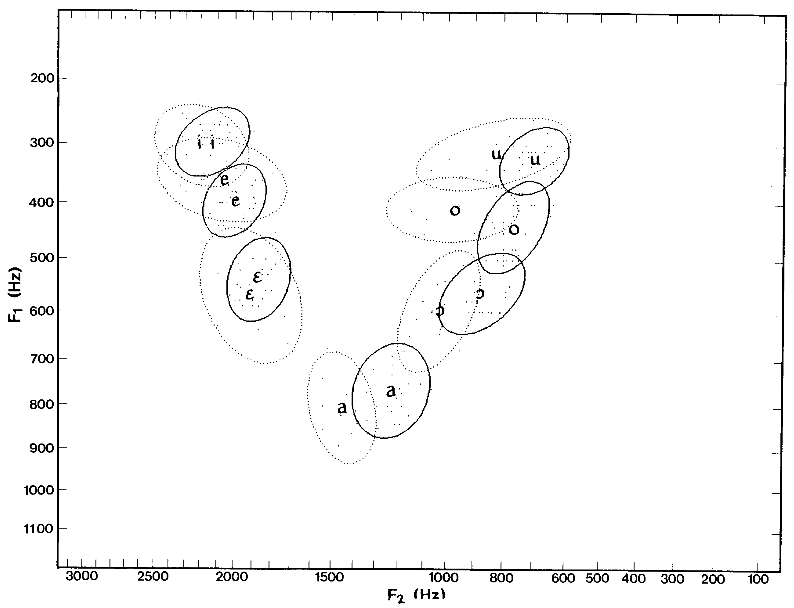
\includegraphics[width=0.75\textwidth]{imagespresentation/vowel_system_yoruba_italian.png}
  \caption{Shared vowels of Yoruba (dotted) and Italian (solid) \citep{ferrari1983}.}
  \label{fig:vowel_system_yoruba_italian}
  \end{figure}
}

\frame
{
  \frametitle{Vowel system: German x Dutch}
  \begin{figure}[h!]
  \centering
  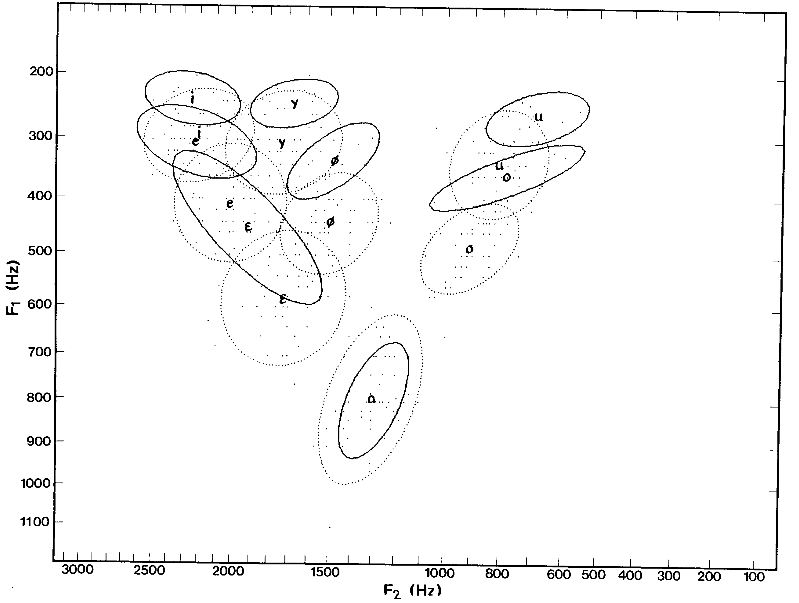
\includegraphics[width=0.75\textwidth]{imagespresentation/vowel_system_german_dutch.png}
  \caption{Shared vowels of German (solid) and Dutch (dotted) \citep{ferrari1983}.}
  \label{fig:vowel_system_german_dutch}
  \end{figure}
}


\frame
{
  \frametitle{Language Structure - Combinations}
  Phonemic Rules
  
  \vspace{0.5cm}
  The consonantal cluster \textipa{[ts]} in
  \begin{description}
  \item[German] is allowed. \\ examples: `Konferenz' (\textipa{[kOnfe'rEnts]}), `Zeit' (\textipa{[tsaIt]}), `umziehen' (\textipa{['PUmtsi:@n]})
  \item[English] is allowed only in word final. \\ examples: `cats' (\textipa{[k\ae ts]}), `splits' (\textipa{[splits]})
  \item[Classical Arabic] no multiconsonant onsets are allowed at all.
  %\item[Portuguese] is not allowed.
  \end{description}
}
\note{
We observe that speech inventory among languages is quite diverse, but there seems to exist some cornerstones
and some patterns that are preferred over others.
Phonemic rules are also different among different languages, creating different patterns, but some
of them are more frequent.

\vspace{0.5cm}
It is important to investigate and understand what the reasons, what are the ubiquitous patterns and
from this knowledge formulate/construct an explanation for how language works. 

\vspace{0.5cm}
Classical Arabic, also known as Quranic Arabic, is the form of the Arabic language used in 
literary texts from Umayyad and Abbasid times (7th to 9th centuries). 
It is based on the Medieval dialects of Arab tribes. Modern Standard Arabic (MSA) is the 
direct descendant used today throughout the Arab World in writing and in formal speaking.
}


\frame
{
  \frametitle{Language Structure, Usage and Representation}
  \begin{figure}[h!]
  \centering
  %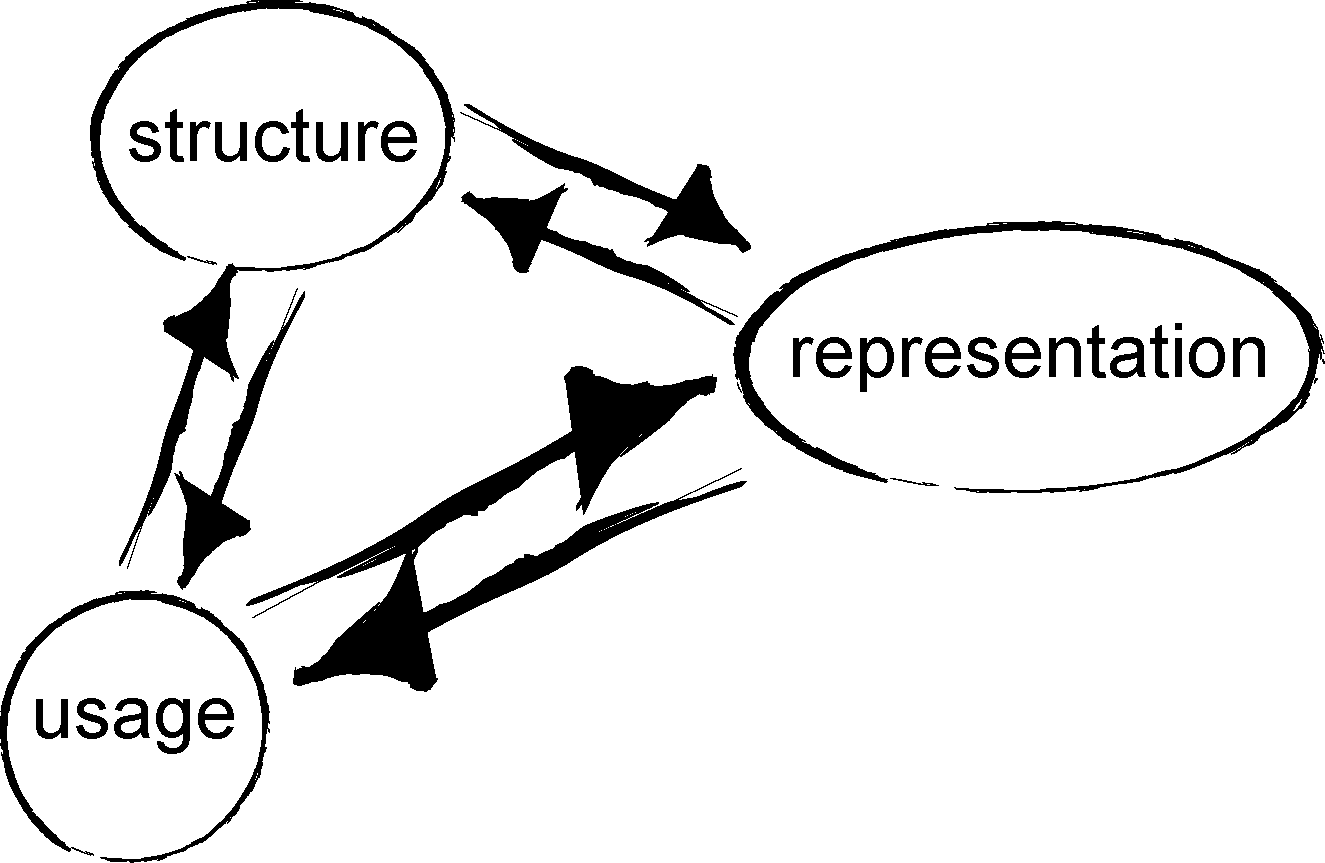
\includegraphics[width=0.95\textwidth]{images/usage_representation_structure.pdf}
  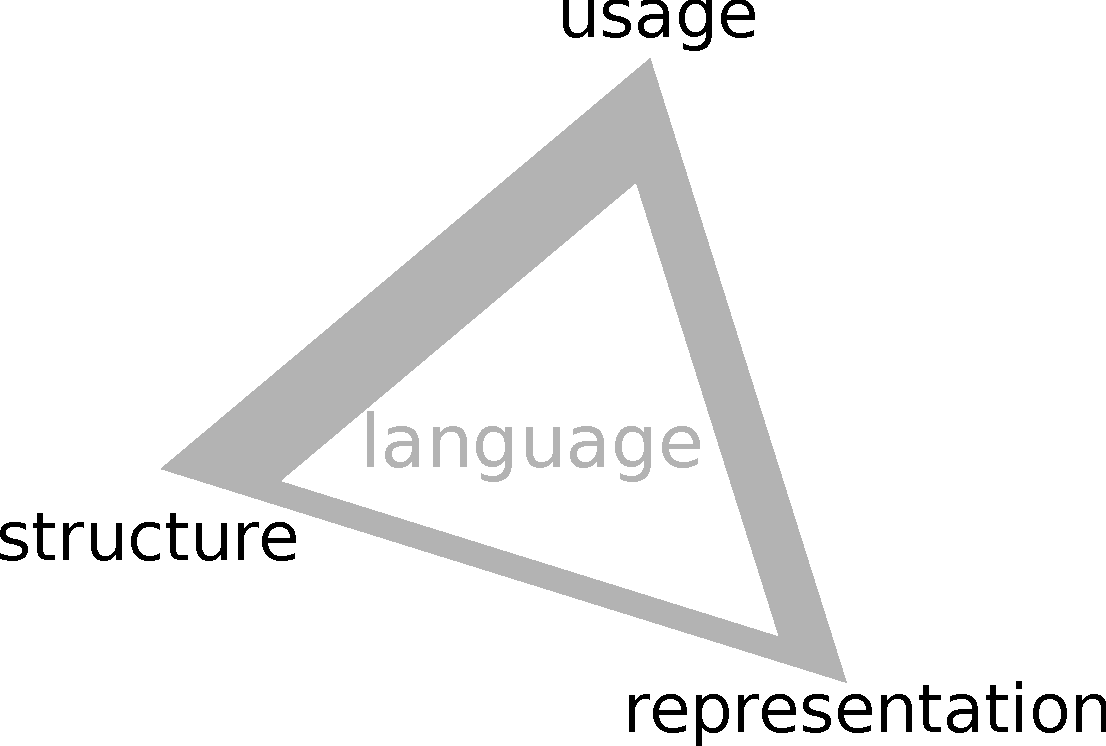
\includegraphics[width=0.75\textwidth]{imagespresentation/triangle.pdf}
  %\caption{}
  \label{fig:usage_representation_structure}
  \end{figure} 
}
\note{
``In particular, the frequency with which individual words or sequences of words are used and the frequency with which certain patterns recur in a language affects the nature of mental representation and in some cases the actual phonetic shape of words''\citep{bybee2003}.

``It is certainly possible that the way language is used affects the way it is represented cognitively, and thus the way it is structured''\citep{bybee2003}.

``The proposal that frequency of use affects representation suggests a very different view of lexical storage and its interaction with other aspects of the grammar or phonology than that assumed in most current theories. Structuralist and generative theories assume that the lexicon is a static list, and that neither the rules nor the lexical forms of a language are changed at all by instances of use''\citep{bybee2003}.
}



\frame
{
  \frametitle{Frequency and Complexity}
  Frequency of occurrence is inversely proportional to complexity
  \citep{zipf1949}.
  
  \begin{itemize}
  \item words
  \item phones, clusters 
  \item within a language or among various languages of the world
  \end{itemize}
  
  \vspace{1cm}
  Complexity and occurrence are intrinsically related to the way languages change.
}
\note{
\cite{zipf1949} proposes that the frequency a phoneme in a language occurs is inversely proportional to its complexity. 
The frequency of clusters should also be inversely proportional to the complexity of the cluster and
now, the complexity of a cluster needs to be defined by the relation created by its parts.

\vspace{0.5cm}
In the history of any language, the phonemic system undergoes constant changes
that may affect the complexity and occurrence frequency of phonemes.
}




\section{Interlanguage Statistical Analysis}
\frame
{
  \frametitle{UCLA Phonological Segment Inventory Database}
  
  The UCLA Phonological Segment Inventory Database (or UPSID) is a statistical survey of the phoneme inventories in 451 of the world's languages. The database was created by American phonetician Ian Maddieson for the University of California, Los Angeles (UCLA) in 1984 and has been updated several times.
  
  \vspace{1cm}
  \url{http://www.linguistics.ucla.edu/faciliti/sales/software.htm}
  
  \vspace{0.25cm}
  Book: Patterns of sounds \citep{maddieson1884}.
}
\note{
Patterns of Sounds describes the frequency and distributional patterns of the phonemic sounds in a large and representative sample of the world's languages. Questions of the frequency and co-occurrence of the particular segment types are discussed in detail and possible explanations for the patterns observed are evaluated.
}


\subsection{UPSID - Statistical Analysis}
\frame
{
  \frametitle{UPSID - Number of Segments (919)}
  
  \begin{figure}[h!]
  \centering
  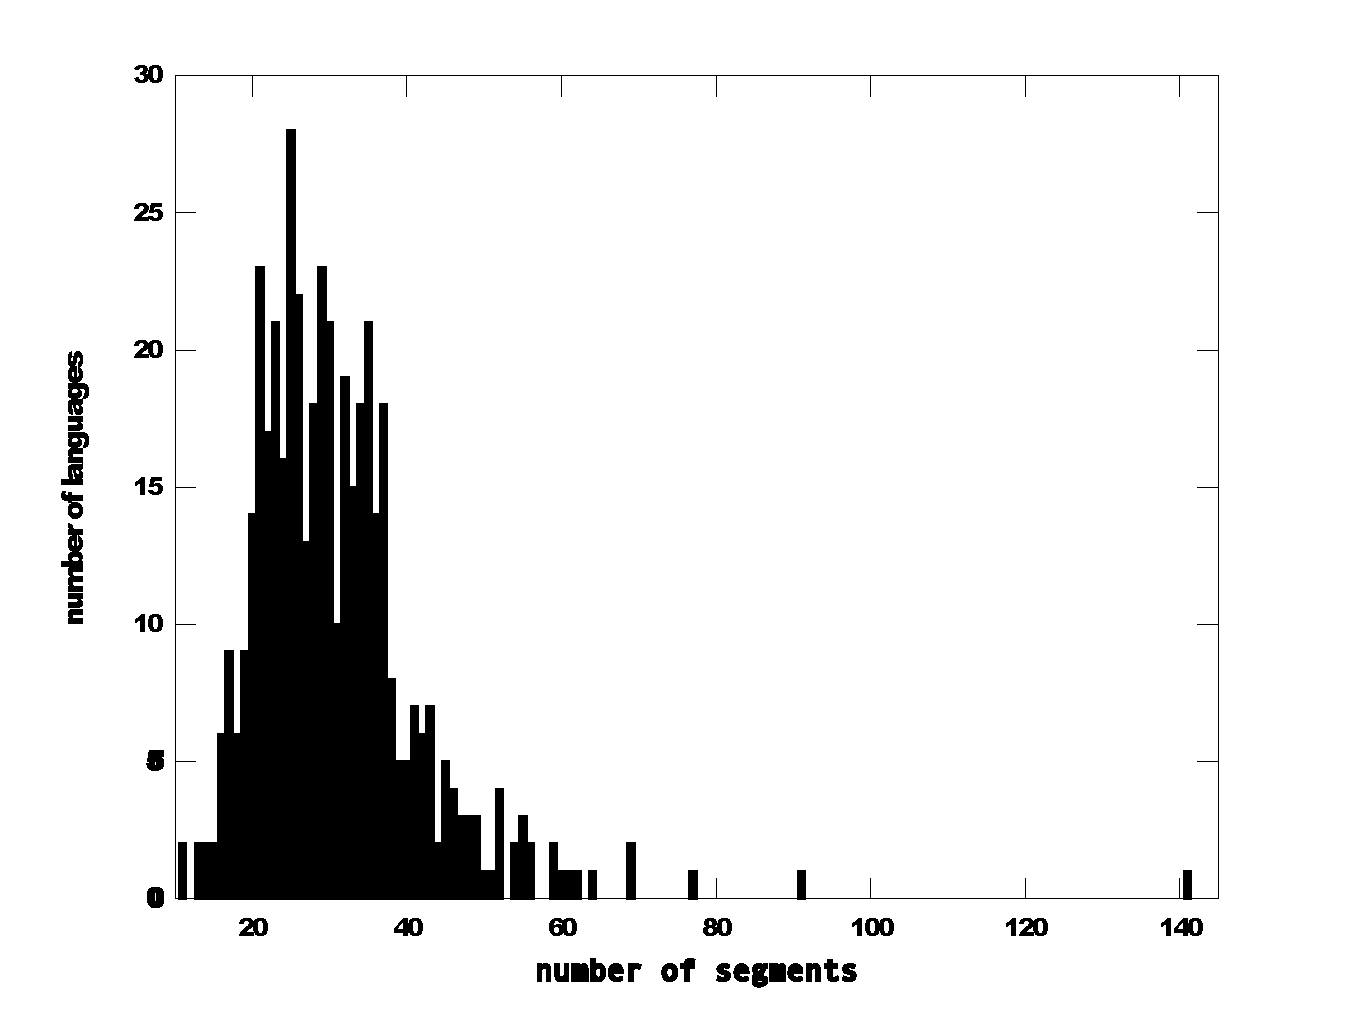
\includegraphics[width=0.7\textwidth]{images/segments_hist_upsid.pdf}
  \caption{Number of phones in various languages of the world.}
  \label{fig:language_segments_hist}
  \end{figure}
}
\note{
Among the 451 languages in the UPSID databese, the minimum number of segments used by a language is 11, in only two languages (Pirah\~a, spoken in Brazil by around 300 speakers; and Rotokas, spoken in Papua New Guinea by approximately 4,300 speakers). The language with the highest number of segments found in the UPSID database has 141 segments (the !Xu language, also called !Kung, is spoken by fifteen thousand speakers in Namibia and Angola). On average, the languages are built on 31 
segments. Figure \ref{fig:language_segments_hist} bellow shows the histogram of languages regarding the number of segments used in each of them.

66.3\% of the languages have a repertoire from 20 to 37 speech sounds.

The languages use between 1.2\% and 15.3\% of all available speech sounds (919).
}


\frame
{
  \frametitle{UPSID - Segments in Languages (451)}
  
  \begin{figure}[h!]
  \centering
  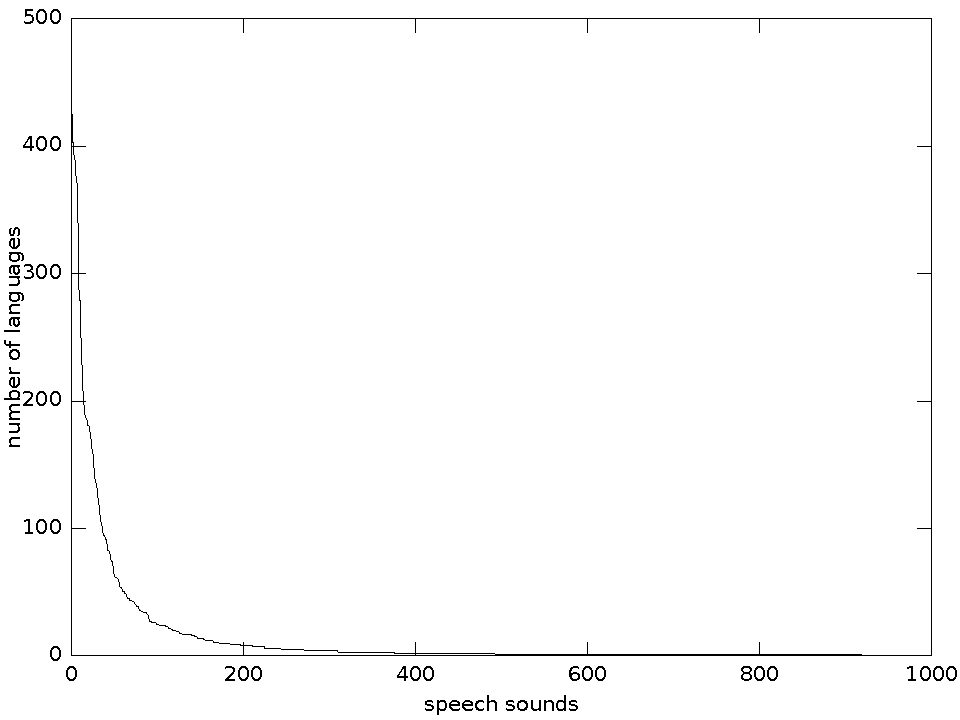
\includegraphics[width=0.7\textwidth]{images/occ_of_speech_sounds_plot.pdf}
  \caption{Number of languages where a give speech sounds occurs.}
  \label{fig:occ_of_speech_sounds_plot}
  \end{figure}
}
\note{
46.5\% of the sounds appear in only one language. 80\% of the sounds appear in 10 or fewer languages.
}

\frame
{
  \frametitle{UPSID - Segments in Languages}

  \begin{figure}[h!]
  \centering
  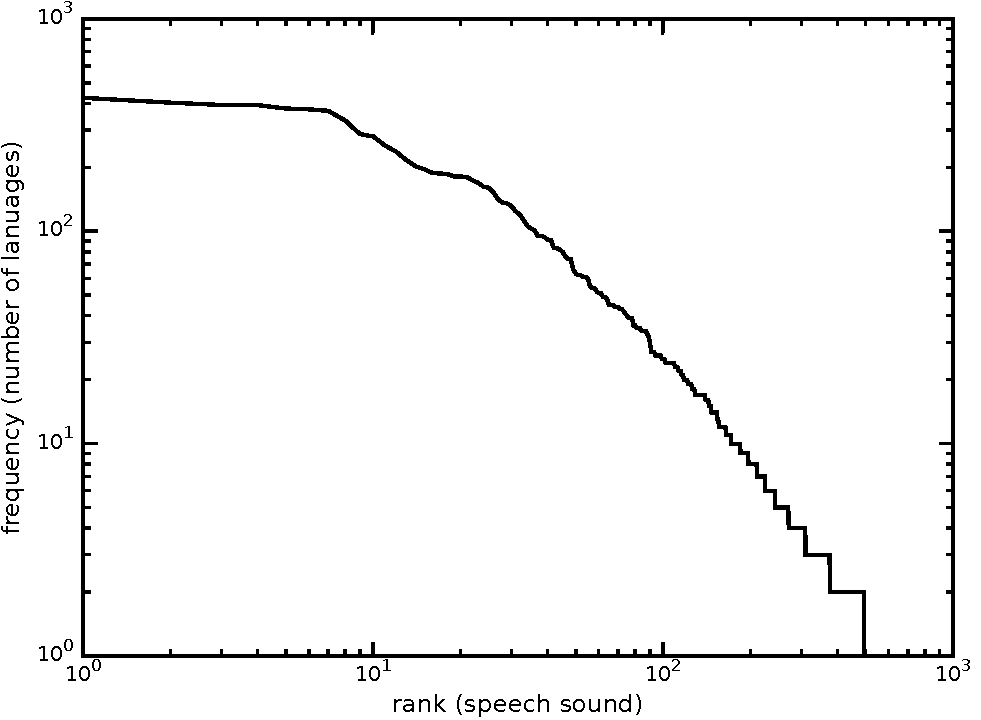
\includegraphics[width=0.7\textwidth]{images/occ_of_speech_sounds_plotlog.pdf}
  \caption{Number of languages for a given speech sound.}
  \label{fig:occ_of_speech_sounds_plotlog}
  \end{figure}
}



\frame
{
  \frametitle{UPSID - Number of Vowels (269)}
  \vspace{-0.3cm}
  \begin{figure}[h!]
  \centering
  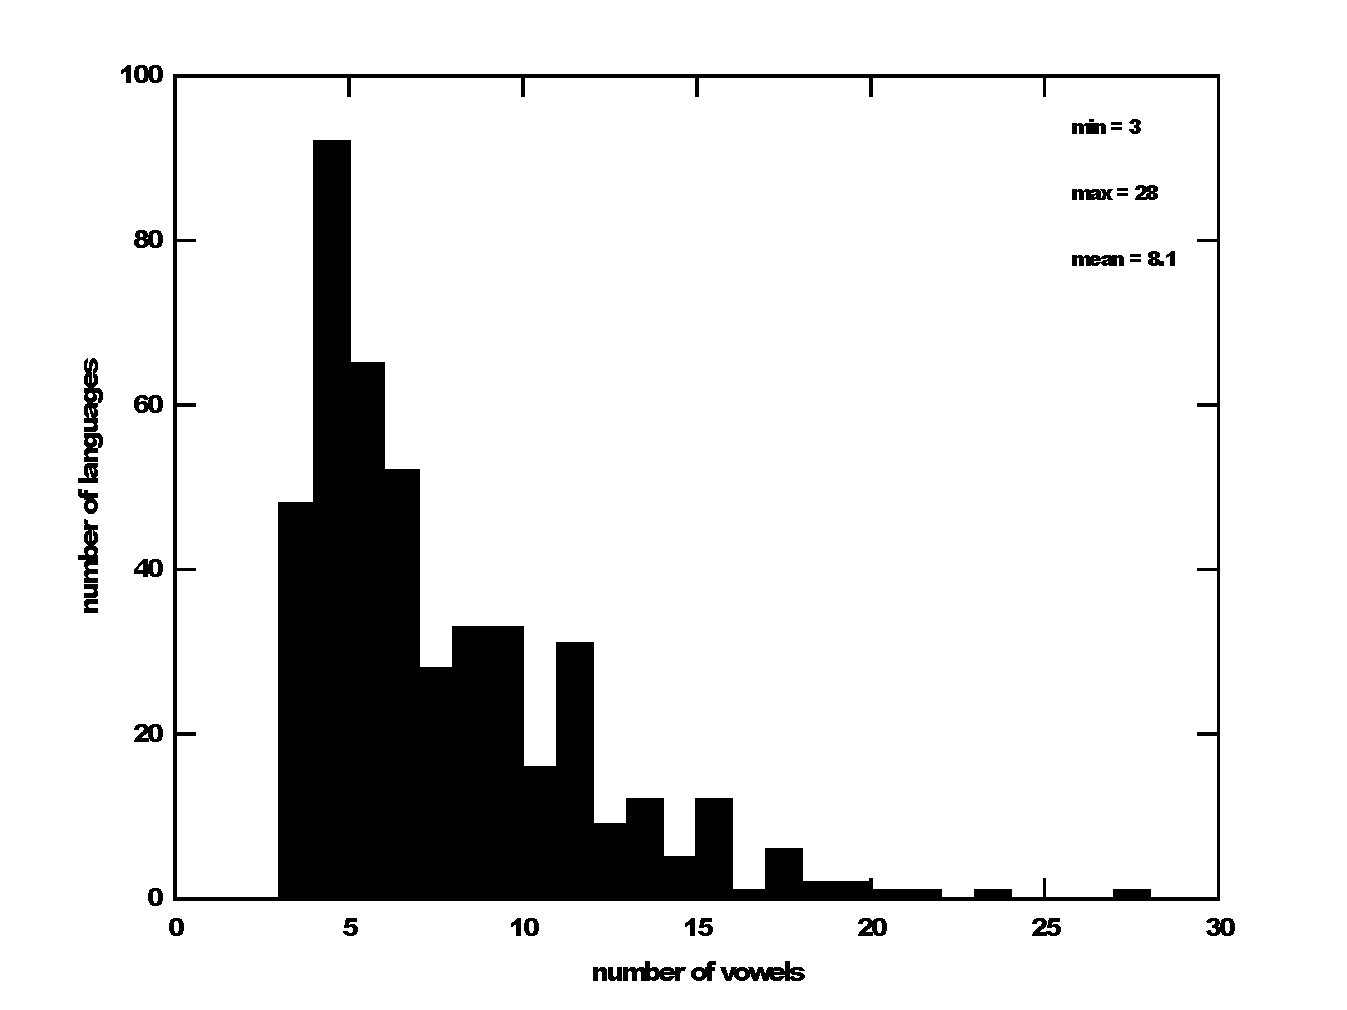
\includegraphics[width=0.8\textwidth]{images/histogram_vowels.pdf}
  \caption{Number of vowels in various languages of the world.}
  \label{fig:histogram_vowels}
  \end{figure}
}
\note{
Considering that the database with 451 languages has in its inventory 652
consonants (71\%) and 269 vowels (29\%), we see that across the languages, the number of vowels used
corresponds from 0.9\% to 17.9\% (averaging 3.0\%) of the possible vowels.
}
 

\frame
{
  \frametitle{UPSID - Number of Consonants (652)}
  \vspace{-0.3cm}
  \begin{figure}[h!]
  \centering
  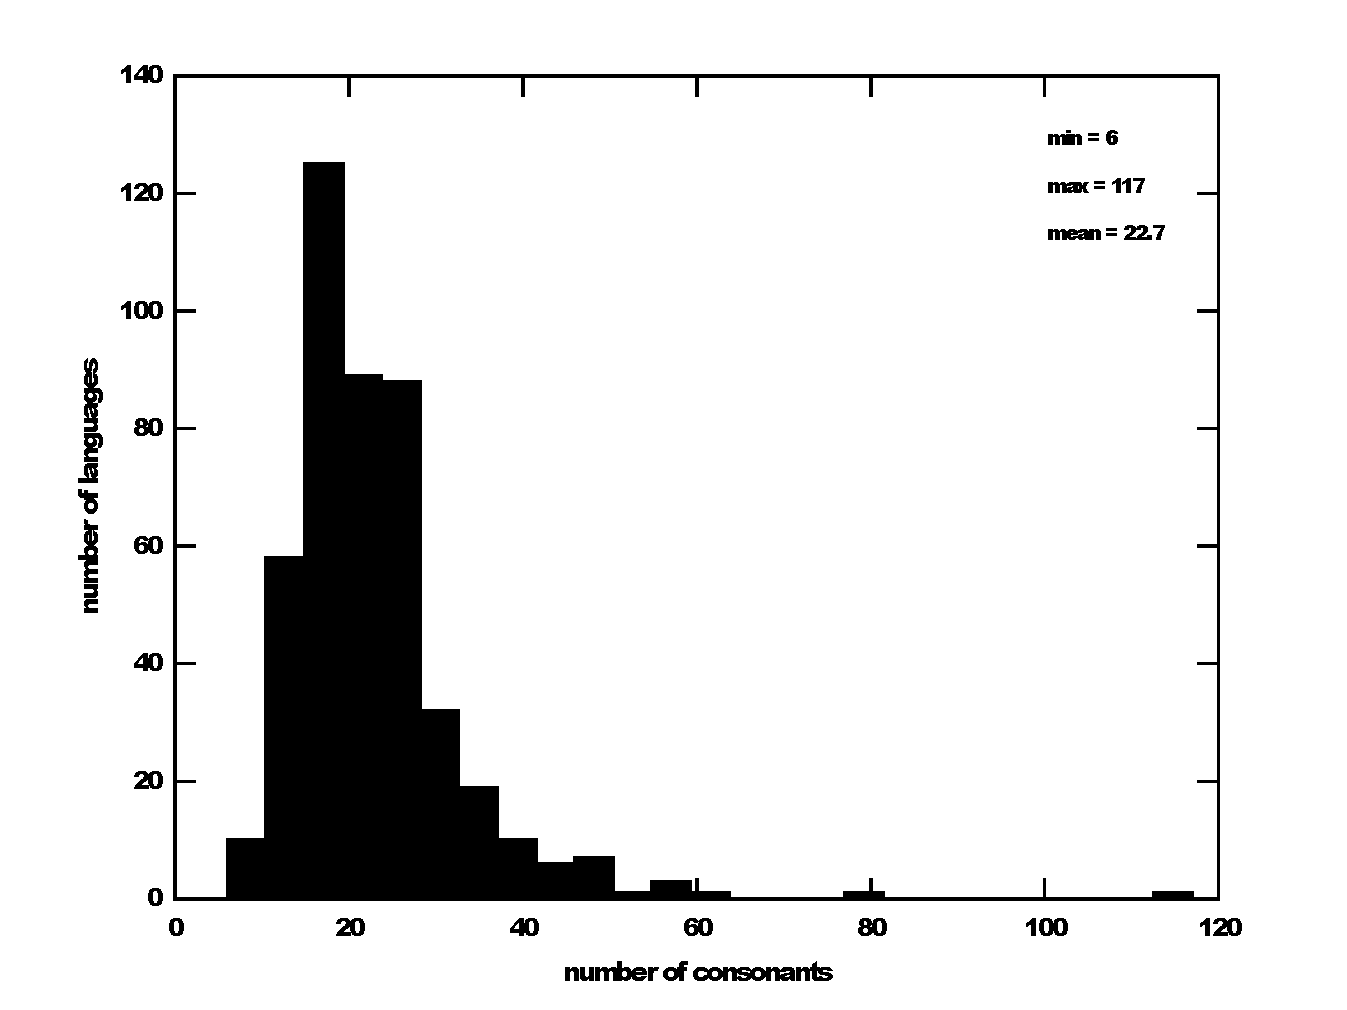
\includegraphics[width=0.8\textwidth]{images/histogram_consonants.pdf}
  \caption{Number of consonants in various languages of the world.}
  \label{fig:histogram_consonants}
  \end{figure}
}
\note{
The number of consonants used goes from 0.9\% to 14.6\% (averaging 3.5\%) of the consonants in the
database (which has an inventory of 652 consonants).
}

\frame
{
  \frametitle{UPSID - Consonant-Vowels Ratio}
  \vspace{-0.3cm}
  \begin{figure}[h!]
  \centering
  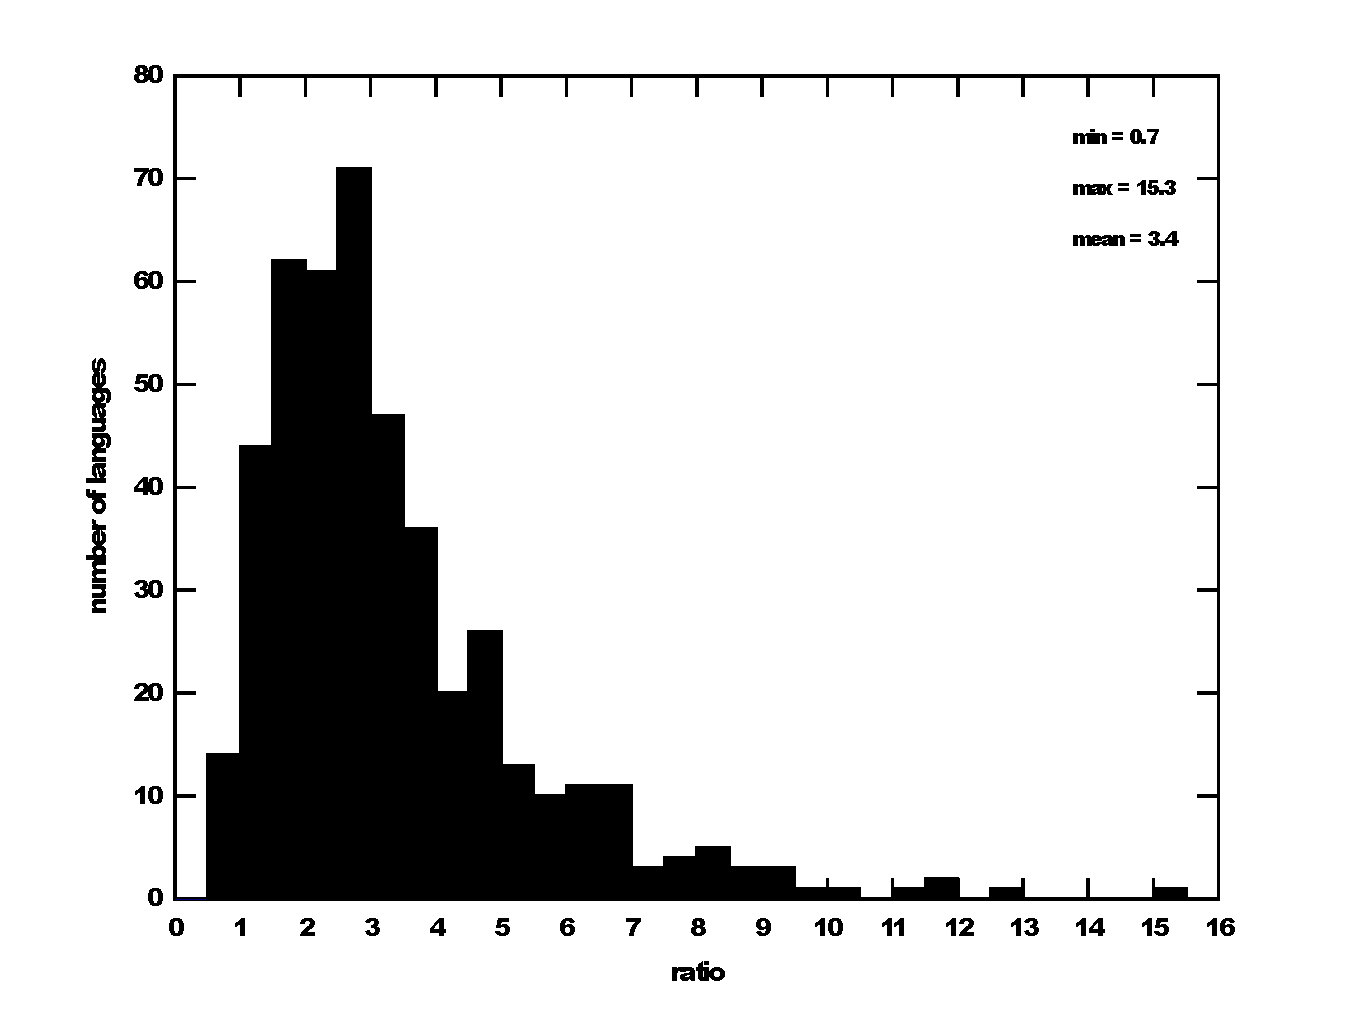
\includegraphics[width=0.8\textwidth]{images/histogram_cv_ratio.pdf}
  \caption{Consonants to Vowel ratio in various languages of the world.}
  \label{fig:histogram_cv_ratio}
  \end{figure}
}
\note{
\begin{multicols}{4}
\begin{itemize}
\item[klao] 0.6875
\item[andoke] 0.73333
\item[vanimo] 0.75
\item[apinaye] 0.76471
\item[dan] 0.85
\item[bruu] 0.90909
\item[barasano] 0.91667
\item[yagua] 0.91667
\item[cubeo] 0.91667
\item[panare] 0.92308
\item[kaingang] 0.92857
\item[kashmiri] 0.96429
\item[japreria] 1
\item[maxakali] 1
\item[(...)]
\item[acoma] 9.2
\item[shilha] 9.3333
\item[coola] 9.3333
\item[yanyuwa] 9.6667
\item[dahalo] 10.2
\item[hadza] 11.4
\item[rutul] 11.8
\item[jaqaru] 12
\item[tsimshian] 12.667
\item[haida] 15.333
\end{itemize}
\end{multicols}
}


\frame
{
  \frametitle{UPSID - Consonant-Vowels Ratio CDF}
  \vspace{-0.3cm}
  \begin{figure}[h!]
  \centering
  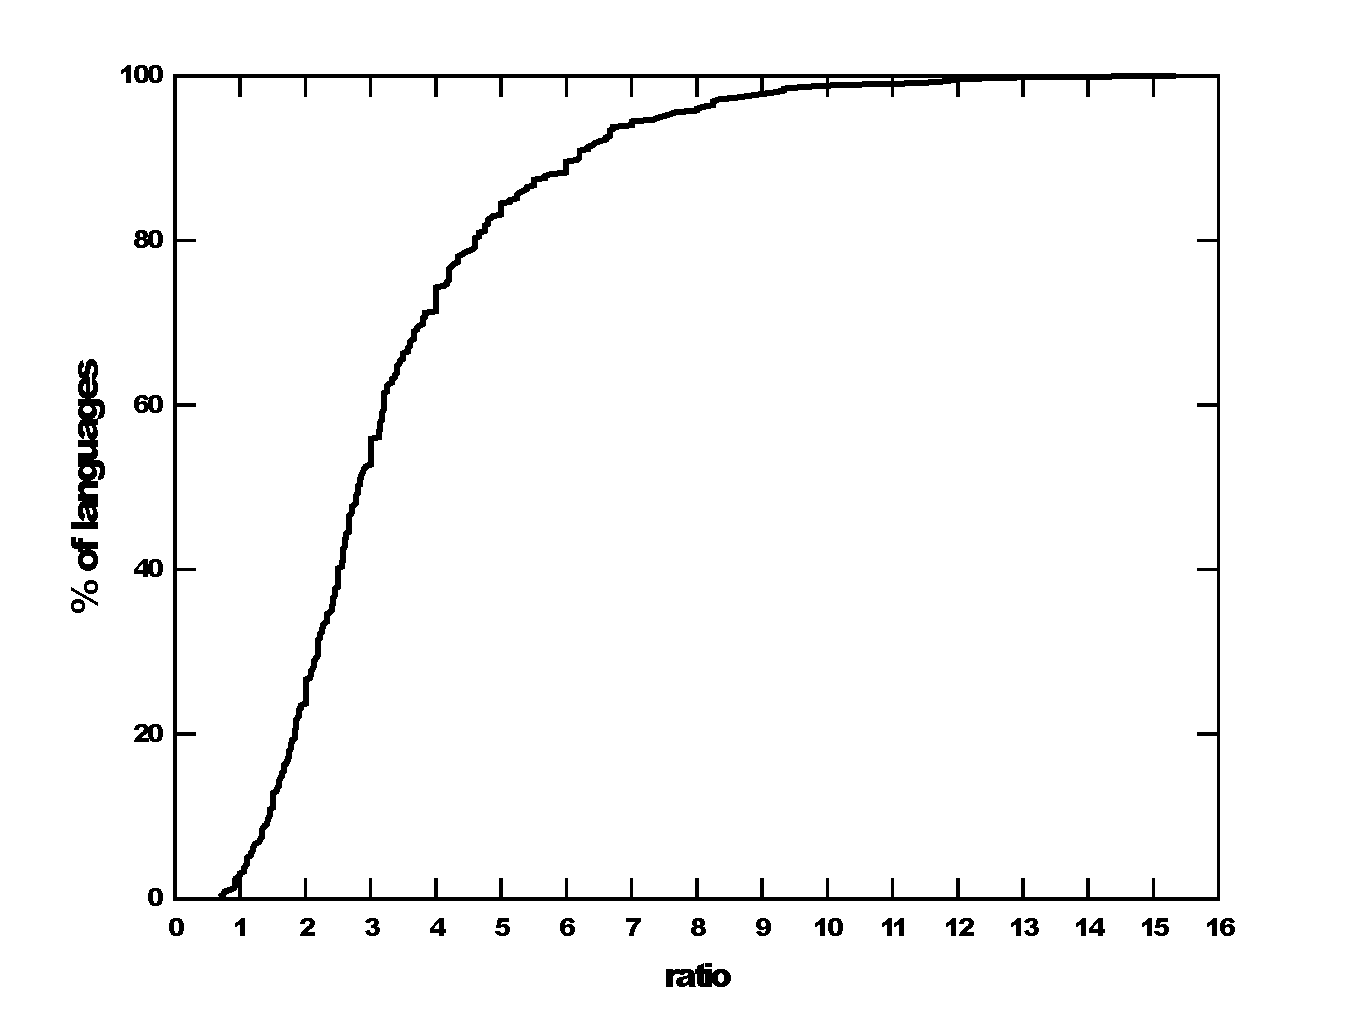
\includegraphics[width=0.8\textwidth]{images/cdf_cv_ratio.pdf}
  \caption{Cumulative distribution of the Consonant-Vowel ratio.}
  \label{fig:cdf_cv_ratio}
  \end{figure}
}



\frame
{
  \frametitle{UPSID - Consonants}
  \begin{table}[h]
  \caption{List of the 20 most frequent consonants in UPSID.}
  \label{tbl:consonants_most_freq}
    
\begin{flushleft}

  \begin{tabular}{|c|c|c|c|c|c|c|c|}
  \hline consonant 		& \textipa{m} & \textipa{k} & \textipa{j} & \textipa{p} & \textipa{w} & \textipa{b} & \textipa{h} \\ 
  \hline n. of languages	& 425 & 403 & 378 & 375 & 332 & 287 & 279 \\ 
  \hline frequency 		& 94.2 & 89.4 & 83.8 & 83.2 & 73.6 & 63.6 & 61.9 \\ 
  \hline 
  \end{tabular} 
  
  \begin{tabular}{|c|c|c|c|c|c|c|c|}
  \hline consonant 		& \textipa{g} & \textipa{N} & \textipa{P} & \textipa{n} & \textipa{s} & \textipa{tS} &   \textipa{S} \\ 
  \hline n. of languages	 & 253 & 237 & 216 & 202 & 196 & 188 & 187 \\ 
  \hline frequency 		& 56.1 & 52.6 & 47.9 & 44.8 & 43.5 & 41.7 & 41.5 \\ 
  \hline 
  \end{tabular} 

  \begin{tabular}{|c|c|c|c|c|c|c|}
  \hline consonant 		& \textipa{t} & \textipa{f} & \textipa{l} & \textipa{\|[n} & \textipa{\|[t} & \textipa{\textltailn } \\ 
  \hline n. of languages	& 181 & 180 & 174 & 160 & 152 & 141 \\ 
  \hline frequency 		 & 40.1 & 39.9 & 38.6 & 35.5 & 33.7 & 31.3 \\ 
  \hline 
  \end{tabular} 
\end{flushleft}    
  
  \end{table}
}


\frame
{
  \frametitle{UPSID - Vowels}
  \begin{table}[h]
  \caption{List of the 10 most frequent vowels in UPSID.}
  \label{tbl:vowels_most_freq}
  \begin{tabular}{|c|c|c|c|c|c|}
  \hline vowel 		& \textipa{i} & \textipa{a} & \textipa{u} & \textipa{E} & \textipa{o/O} \\ 
  \hline n. of languages	& 393 & 392 & 369 & 186 & 181  \\ 
  \hline frequency 		& 87.1 & 86.9 & 81.8 & 41.2 & 40.1 \\ 
  \hline 
  \end{tabular} 
  
  \begin{tabular}{|c|c|c|c|c|c|}
  \hline vowel 		& \textipa{e/E} & \textipa{O} & \textipa{o} & \textipa{e} & \textipa{~a} \\ 
  \hline n. of languages	& 169 & 162 & 131 & 124 & 83 \\ 
  \hline frequency 		& 37.5 & 35.9 & 29.0 & 27.5 & 18.4 \\ 
  \hline 
  \end{tabular} 
  \end{table}
}
\note{
The most frequent vowels are not so frequent across languages in comparison to the most frequent consonants.
}


\frame
{
  \frametitle{UPSID - number of phones vs. frequency index}
  \begin{figure}[h!]
  \centering
  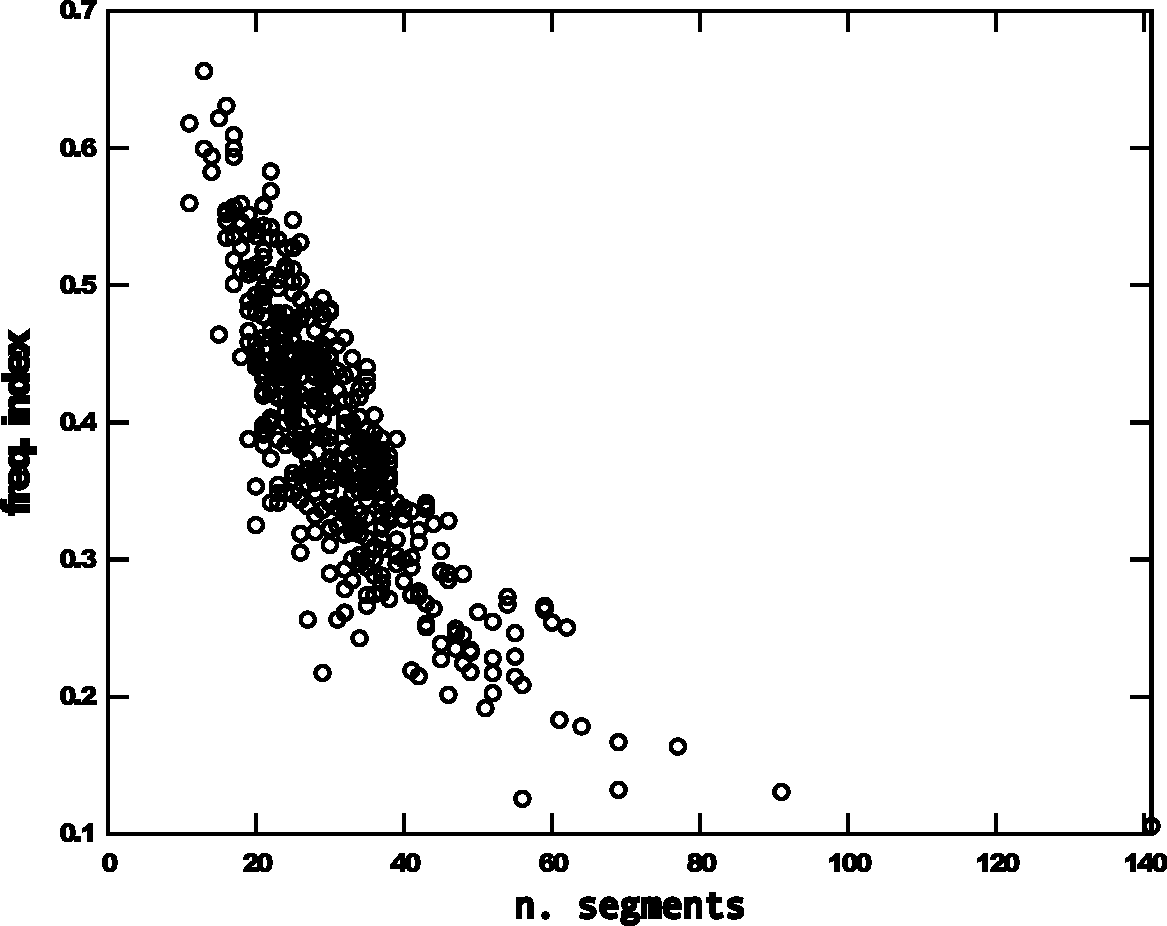
\includegraphics[width=0.7\textwidth]{images/freqidx_nsegs_upsid.pdf}
  \caption{Relation between the frequency index and the number of phones in a language. (Data from UPSID)}
  \label{fig:freqidx_nsegs_upsid}
  \end{figure} 
}
\note{
Frequency index is the arithmetic average of the segment frequencies of a language. 
A language with mostly rare segments will have a low frequency index, 
whereas a language with mostly common sounds will have a high frequency index. 
A frequency index of 0.1 means that a language has many very rare segments; 
0.7 means it has many common segments; the average frequency index of all languages is 0.39. 
}
\note{
Note that there is a relation between frequency index and number of segments in a language. 
That is, if a language has only few segments, it is likely that these are rather common in the languages in UPSID. 
On the other hand, a language with many segments will also have many segments that are uncommon in the UPSID database. 
This does not necessarily mean that certain sounds are more natural but it is a probabilistic effect: 
if you make a pot with many red marbles, few green marbles, and other marbles with different colors and you draw 
a small random sample (i.e. 10 marbles) you will have mostly red marbles. If you draw a large random sample 
(e.g. 100 marbles) you will have many single colored ones. 
  
Frequency index: mean=0.39, max=0.66, min=0.11.
}



\frame
{
  \frametitle{UPSID - cooccurrence of phones in a language}

     \vspace{-0.5cm}
     \hvFloat[%
     floatPos=htb,%
     capWidth=1.0,%
     capPos=l,%
     capVPos=t,%
     ]{figure}{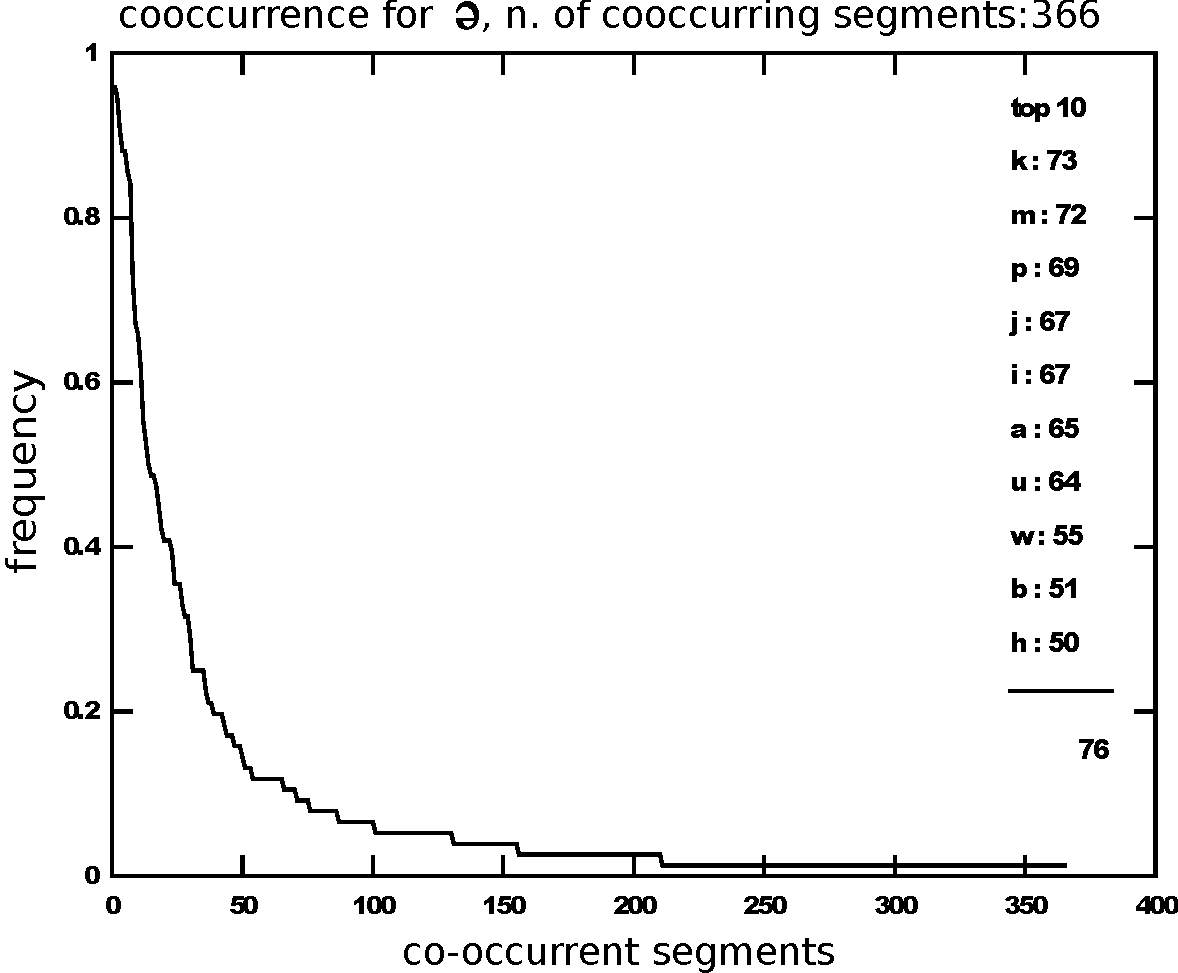
\includegraphics[width=0.75\textwidth]{imagespresentation/cooccurrence_01.pdf}}{\begin{footnotesize}Co-occurrence frequency for phones in relation to \textipa{[@]}. \textipa{[@]} occurs in 76 languages (16.8\%) and has 366 cooccurring phones (39.8\%). Cooccurring phones: \newline \textipa{[k]} (96.0\%), \newline \textipa{[m]} (94.7\%), \newline \textipa{[p]} (90.7\%), etc. \end{footnotesize}}{fig:cooccurrence_01}  
}
\note{
This graph presents the co-occurrence frequency for phones in relation to \textipa{[@]}. The phone \textipa{[@]} occurs in 76 languages (16.8\%). It has 366 cooccurring phones in UPSID, that means 39.8\% of 919 phones. Among them, the phone \textipa{[k]} has a frequency of 96.0\% (73/76). \textipa{[m]} follows with 94.7\% (72/76) and \textipa{[p]} with 90.7\% (69/76).
}



\frame
{
  \frametitle{UPSID - cooccurrence of phones in a language}

     \vspace{-0.5cm}
     \hvFloat[%
     floatPos=htb,%
     capWidth=1.0,%
     capPos=l,%
     capVPos=t,%
     ]{figure}{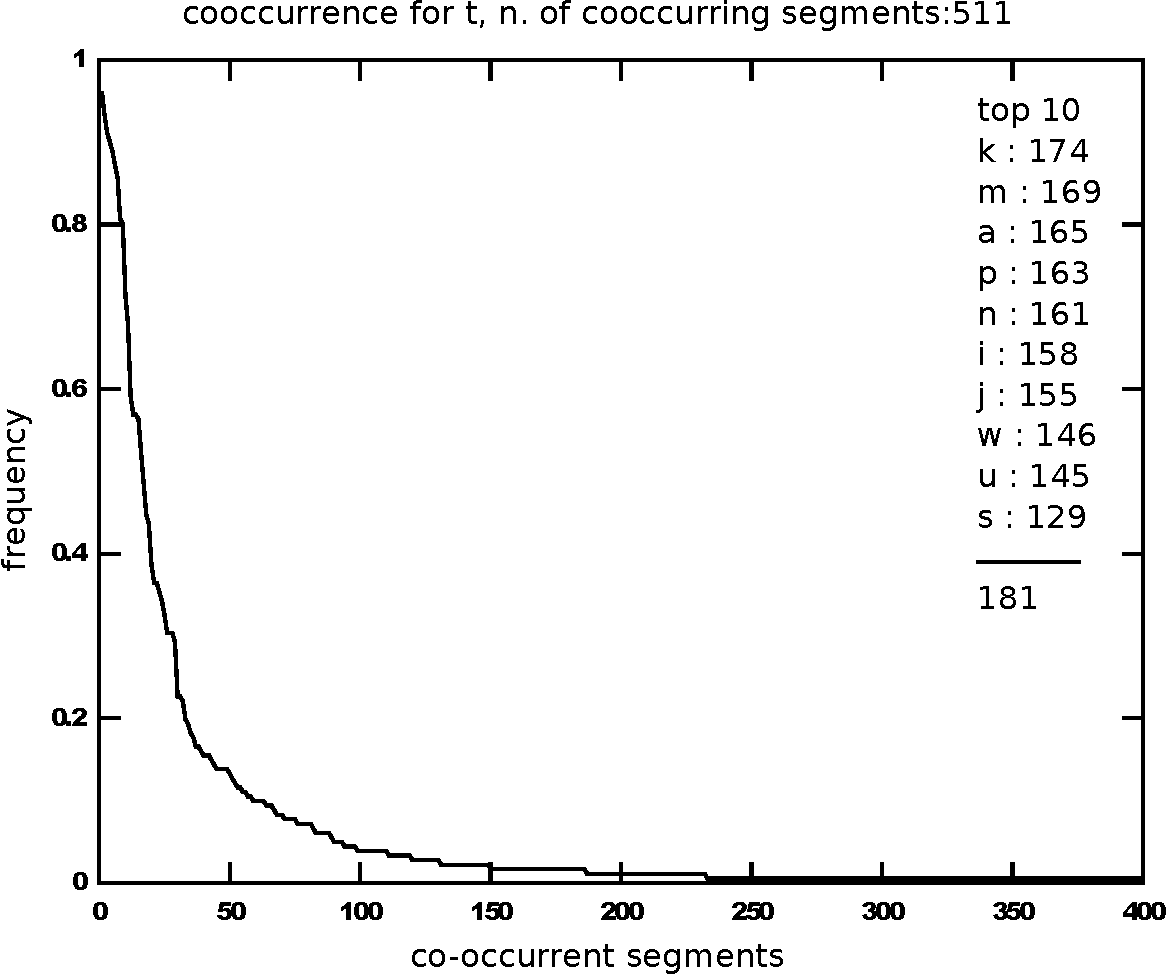
\includegraphics[width=0.75\textwidth]{imagespresentation/cooccurrence_02.pdf}}{\begin{footnotesize}Co-occurrence frequency for phones in relation to \textipa{[t]}. \textipa{[t]} occurs in 181 languages (40.1\%) and has 511 cooccurring phones (55.6\%). Cooccurring phones: \newline \textipa{[k]} (96.1\%), \newline \textipa{[m]} (93.3\%), \newline \textipa{[a]} (91.2\%), etc.\end{footnotesize}}{fig:cooccurrence_02}  
}

\frame
{
  \frametitle{UPSID - cooccurrence of phones in a language}

     \vspace{-0.5cm}
     \hvFloat[%
     floatPos=htb,%
     capWidth=1.0,%
     capPos=l,%
     capVPos=t,%
     ]{figure}{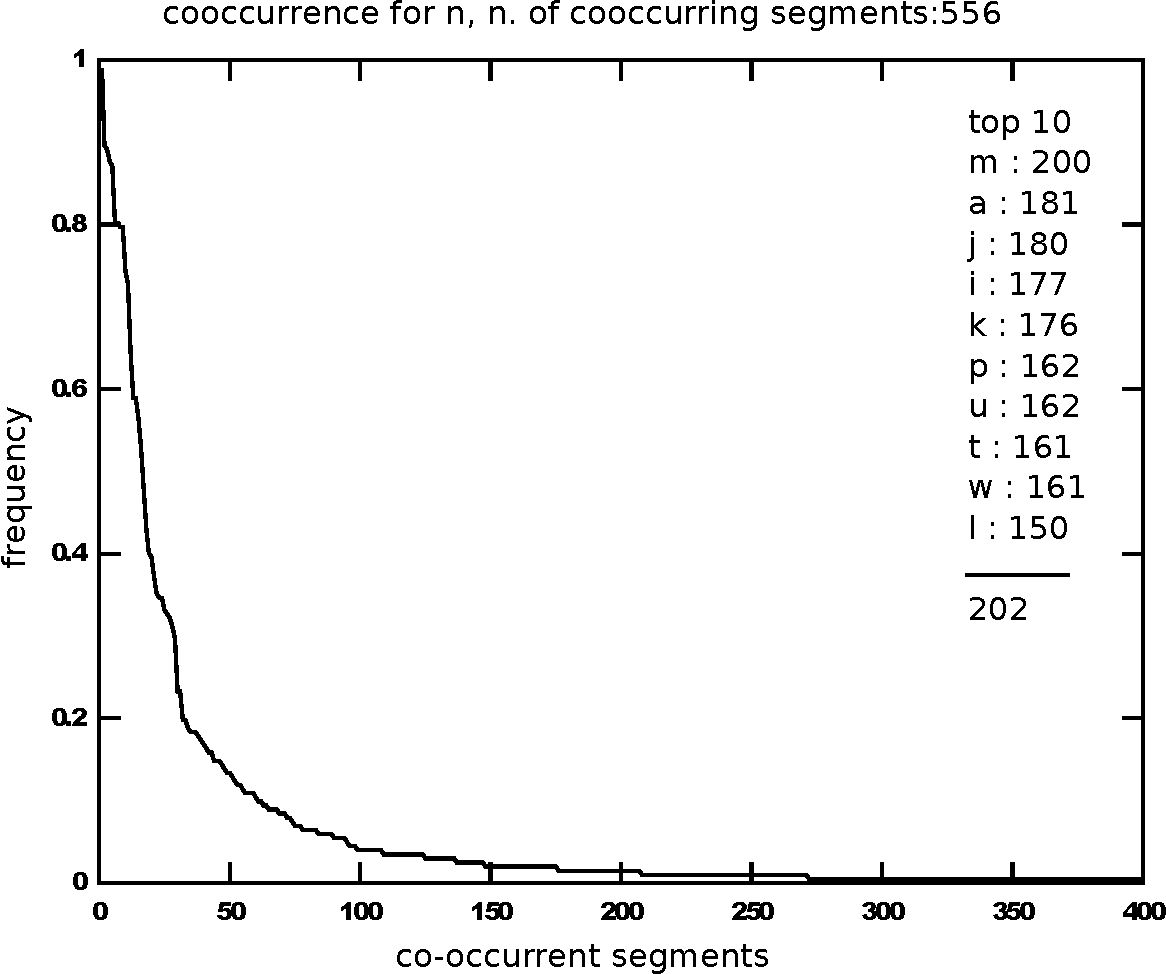
\includegraphics[width=0.75\textwidth]{imagespresentation/cooccurrence_03.pdf}}{\begin{footnotesize}Co-occurrence frequency for phones in relation to \textipa{[n]}. \textipa{[n]} occurs in 202 languages (44.7\%) and has 556 cooccurring phones (60.5\%). Cooccurring phones: \newline \textipa{[m]} (99.0\%), \newline \textipa{[a]} (89.6\%), \newline \textipa{[j]} (89.1\%), etc.\end{footnotesize}}{fig:cooccurrence_03}  
}

\frame
{
  \frametitle{UPSID - cooccurrence of phones in a language}

     \vspace{-0.5cm}
     \hvFloat[%
     floatPos=htb,%
     capWidth=1.0,%
     capPos=l,%
     capVPos=t,%
     ]{figure}{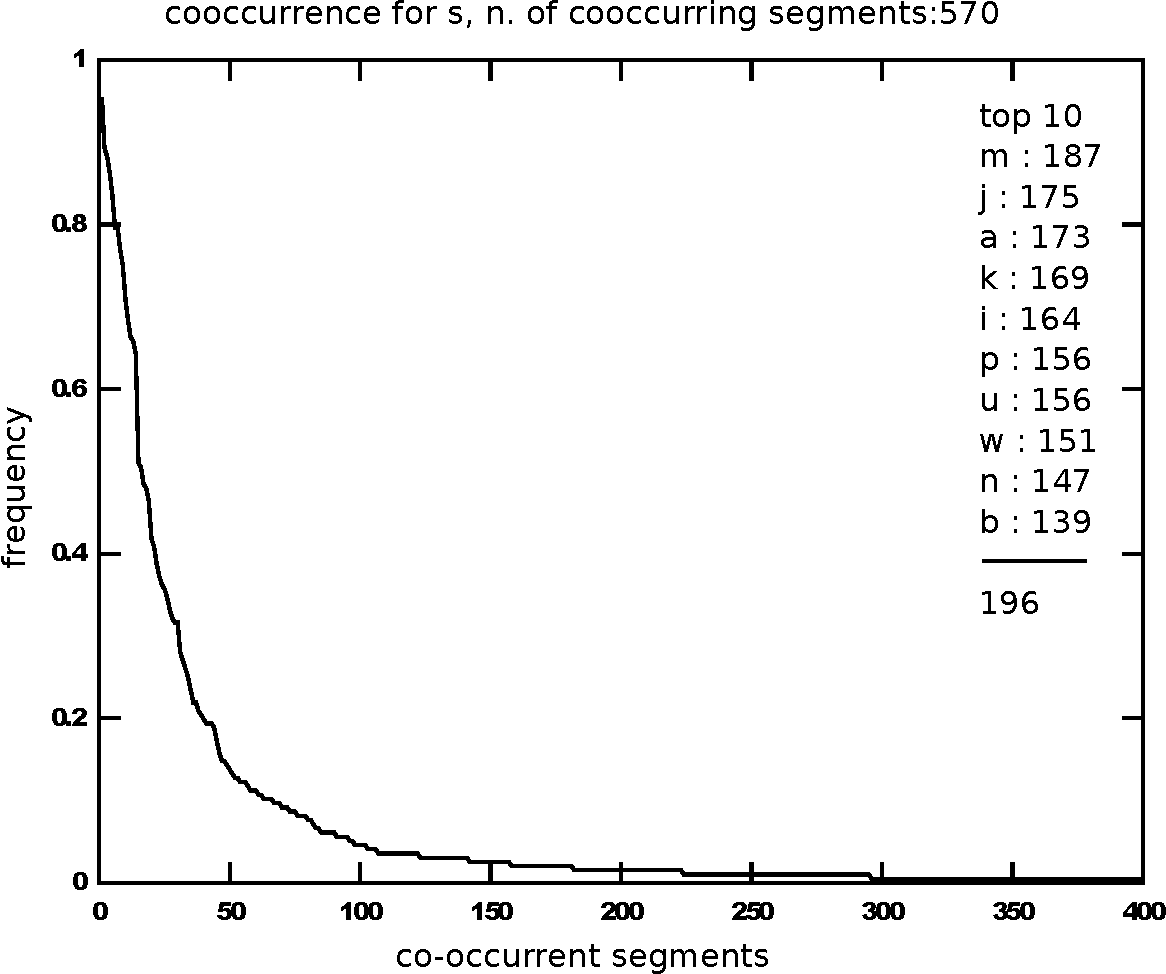
\includegraphics[width=0.75\textwidth]{imagespresentation/cooccurrence_05.pdf}}{\begin{footnotesize}Co-occurrence frequency for phones in relation to \textipa{[s]}. \textipa{[s]} occurs in 196 languages (43.5\%) and has 570 cooccurring phones (62.0\%). Cooccurring phones: \newline \textipa{[m]} (95.4\%), \newline \textipa{[j]} (89.3\%), \newline \textipa{[a]} (88.3\%), etc.\end{footnotesize}}{fig:cooccurrence_05}  
}

\frame
{
  \frametitle{UPSID - cooccurrence of phones in a language}

     \vspace{-0.5cm}
     \hvFloat[%
     floatPos=htb,%
     capWidth=1.0,%
     capPos=l,%
     capVPos=t,%
     ]{figure}{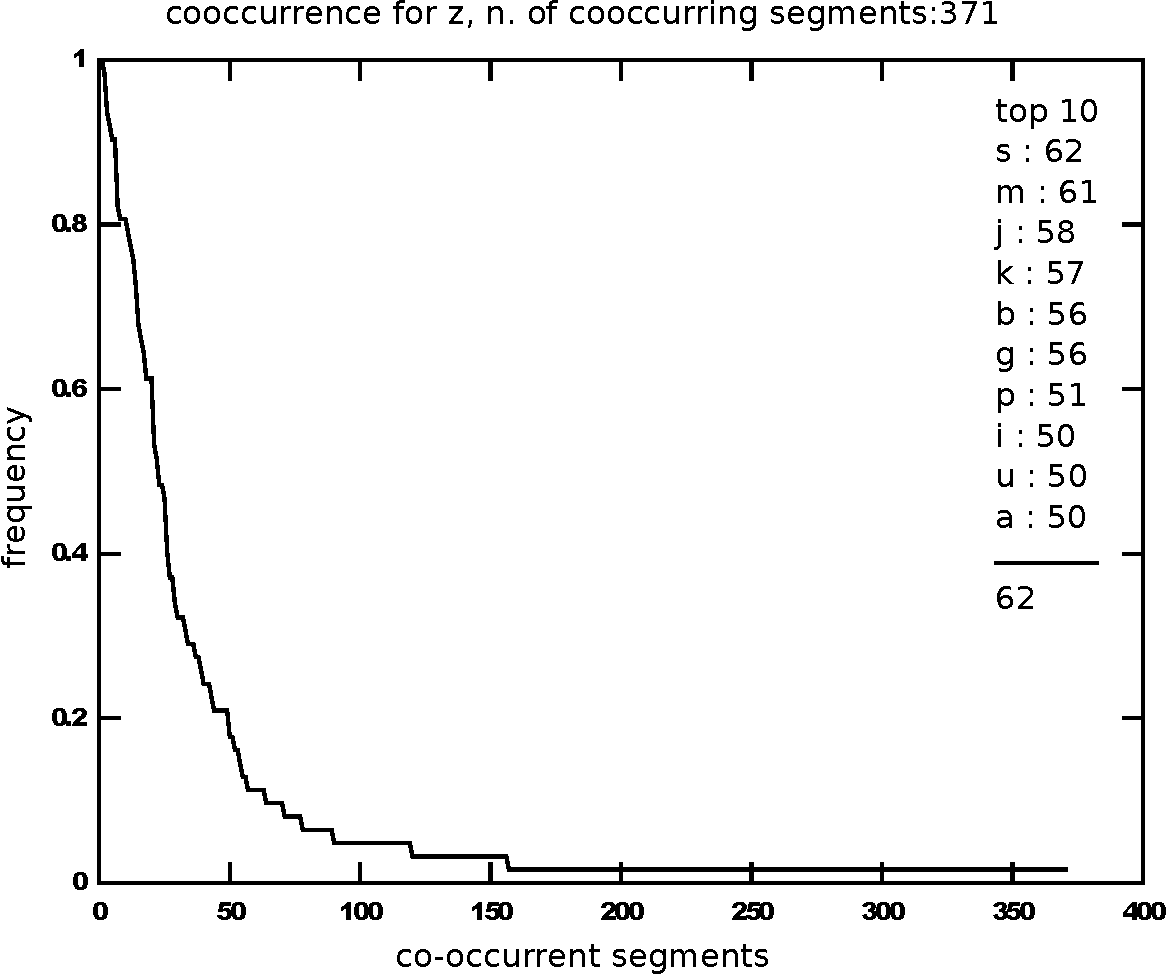
\includegraphics[width=0.75\textwidth]{imagespresentation/cooccurrence_06.pdf}}{\begin{footnotesize}Co-occurrence frequency for phones in relation to \textipa{[z]}. \textipa{[z]} occurs in 62 languages (13.7\%) and has 371 cooccurring phones (40.4\%). Cooccurring phones: \newline \textipa{[s]} (100\%), \newline \textipa{[m]} (98.4\%), \newline \textipa{[j]} (93.5\%), etc.\end{footnotesize}}{fig:cooccurrence_06}  
}
\note{
Always when the phone \textipa{[z]} (voiced alveolar fricatives) is present, the phone \textipa{[s]} (voiceless alveolar fricatives) is also present.
}


\frame
{
  \frametitle{UPSID - cooccurrence of phones in a language}
\vspace{-0.5cm}
\begin{table}[h]
\caption{List of phones and their top 8 co-occurring pairs with their relative frequency of occurrence (data from UPSID).}
\label{tbl:cooccurrence}
\begin{tiny}
\begin{tabular}{|c||c|c|c|c|c|c|c|c|c|}
\hline 
phone & \multicolumn{8}{|c|}{co-occurring phone with their respective relative frequency (\%)} \\  
\hline 
\textipa{@} & \textipa{k} : 96.1 & \textipa{m} : 94.7 & \textipa{p} : 90.8 & \textipa{j} : 88.2 & \textipa{i} : 88.2 & \textipa{a} : 85.5 & \textipa{u} : 84.2 & \textipa{w} : 72.4 \\ \hline
\textipa{t} & \textipa{k} : 96.1 & \textipa{m} : 93.4 & \textipa{a} : 91.2 & \textipa{p} : 90.1 & \textipa{n} : 89.0 & \textipa{i} : 87.3 & \textipa{j} : 85.6 & \textipa{w} : 80.7 \\ \hline
\textipa{n} & \textipa{m} : 99.0 & \textipa{a} : 89.6 & \textipa{j} : 89.1 & \textipa{i} : 87.6 & \textipa{k} : 87.1 & \textipa{p} : 80.2 & \textipa{u} : 80.2 & \textipa{t} : 79.7 \\ \hline
\textipa{I} & \textipa{m} : 97.3 & \textipa{j} : 91.9 & \textipa{k} : 86.5 & \textipa{a} : 83.8 & \textipa{p} : 83.8 & \textipa{U} : 74.3 & \textipa{w} : 71.6 & \textipa{b} : 66.2 \\ \hline
\textipa{s} & \textipa{m} : 95.4 & \textipa{j} : 89.3 & \textipa{a} : 88.3 & \textipa{k} : 86.2 & \textipa{i} : 83.7 & \textipa{p} : 79.6 & \textipa{u} : 79.6 & \textipa{w} : 77.0 \\ \hline
\textipa{z} & \textipa{s} : 100.0 & \textipa{m} : 98.4 & \textipa{j} : 93.5 & \textipa{k} : 91.9 & \textipa{b} : 90.3 & \textipa{g} : 90.3 & \textipa{p} : 82.3 & \textipa{i} : 80.6 \\ \hline
\textipa{d} & \textipa{b} : 96.7 & \textipa{m} : 94.2 & \textipa{i} : 91.7 & \textipa{a} : 90.8 & \textipa{j} : 90.0 & \textipa{n} : 89.2 & \textipa{g} : 87.5 & \textipa{u} : 86.7 \\ \hline
\textipa{l} & \textipa{m} : 98.9 & \textipa{j} : 89.1 & \textipa{k} : 86.8 & \textipa{n} : 86.2 & \textipa{a} : 86.2 & \textipa{i} : 85.6 & \textipa{p} : 81.0 & \textipa{w} : 79.9 \\ \hline
\textipa{i} & \textipa{m} : 93.9 & \textipa{u} : 91.6 & \textipa{k} : 89.6 & \textipa{a} : 89.1 & \textipa{p} : 82.7 & \textipa{j} : 82.7 & \textipa{w} : 73.8 & \textipa{b} : 65.1 \\ \hline
\textipa{\|[d} & \textipa{b} : 97.5 & \textipa{m} : 96.2 & \textipa{g} : 93.8 & \textipa{j} : 88.8 & \textipa{k} : 85.0 & \textipa{\|[t} : 83.8 & \textipa{i} : 80.0 & \textipa{p} : 76.2 \\ \hline
\textipa{m} & \textipa{k} : 89.2 & \textipa{i} : 86.8 & \textipa{a} : 86.6 & \textipa{j} : 85.2 & \textipa{p} : 82.6 & \textipa{u} : 81.6 & \textipa{w} : 74.1 & \textipa{b} : 64.2 \\ \hline
\textipa{n} & \textipa{m} : 99.0 & \textipa{a} : 89.6 & \textipa{j} : 89.1 & \textipa{i} : 87.6 & \textipa{k} : 87.1 & \textipa{p} : 80.2 & \textipa{u} : 80.2 & \textipa{t} : 79.7 \\ \hline
\textipa{k} & \textipa{m} : 94.0 & \textipa{p} : 91.3 & \textipa{i} : 87.3 & \textipa{a} : 86.6 & \textipa{j} : 83.4 & \textipa{u} : 82.1 & \textipa{w} : 73.2 & \textipa{b} : 62.8 \\ \hline
\textipa{g} & \textipa{b} : 96.4 & \textipa{m} : 95.3 & \textipa{i} : 89.3 & \textipa{j} : 87.4 & \textipa{k} : 86.2 & \textipa{u} : 84.2 & \textipa{a} : 83.0 & \textipa{p} : 76.7 \\ \hline
\textipa{p} & \textipa{k} : 98.1 & \textipa{m} : 93.6 & \textipa{a} : 87.2 & \textipa{i} : 86.7 & \textipa{j} : 82.9 & \textipa{u} : 81.3 & \textipa{w} : 71.7 & \textipa{b} : 60.5 \\ \hline
\textipa{b} & \textipa{m} : 95.1 & \textipa{i} : 89.2 & \textipa{k} : 88.2 & \textipa{j} : 86.8 & \textipa{g} : 85.0 & \textipa{u} : 84.3 & \textipa{a} : 84.3 & \textipa{p} : 79.1 \\ \hline
\textipa{S} & \textipa{m} : 94.7 & \textipa{j} : 91.4 & \textipa{k} : 88.8 & \textipa{i} : 84.0 & \textipa{a} : 82.9 & \textipa{p} : 80.2 & \textipa{u} : 78.1 & \textipa{w} : 74.3 \\ \hline
\textipa{Z} & \textipa{S} : 95.1 & \textipa{m} : 95.1 & \textipa{j} : 90.2 & \textipa{k} : 90.2 & \textipa{b} : 82.0 & \textipa{g} : 80.3 & \textipa{i} : 78.7 & \textipa{p} : 78.7 \\ \hline
\end{tabular} 
\end{tiny}
\end{table}  
}
\note{
As we take one bilabial consonants as reference, the others appear in the top-10 list, showing a strong
adhesion of one bilabial consonant to another. 
Observing now the voiced alveolar sibilant fricative \textipa{[z]}, its voiceless counterpart always appear, but doing the other way around analysis, taking \textipa{[s]} as a reference, its voiced counterpart \textipa{[z]} has a relative frequency of co-occurrence of 31.6\%, figuring as the 29th in the list. 
Analyzing other pairs like \textipa{[t]}-\textipa{[d]} (alveolar plosive), \textipa{[k]}-\textipa{[g]} (velar plosive), \textipa{[p]}-\textipa{[b]} (bilabial plosive) and \textipa{[Z]}-\textipa{[S]} (palato-alveolar fricative), it seems that the existence of the voiced counterpart subjects the existence of the voiceless much more emphatically than the other way around.
}



\frame
{
  \frametitle{UPSID - cooccurrence of phones in a language}
  \begin{figure}[h!]
  \centering
  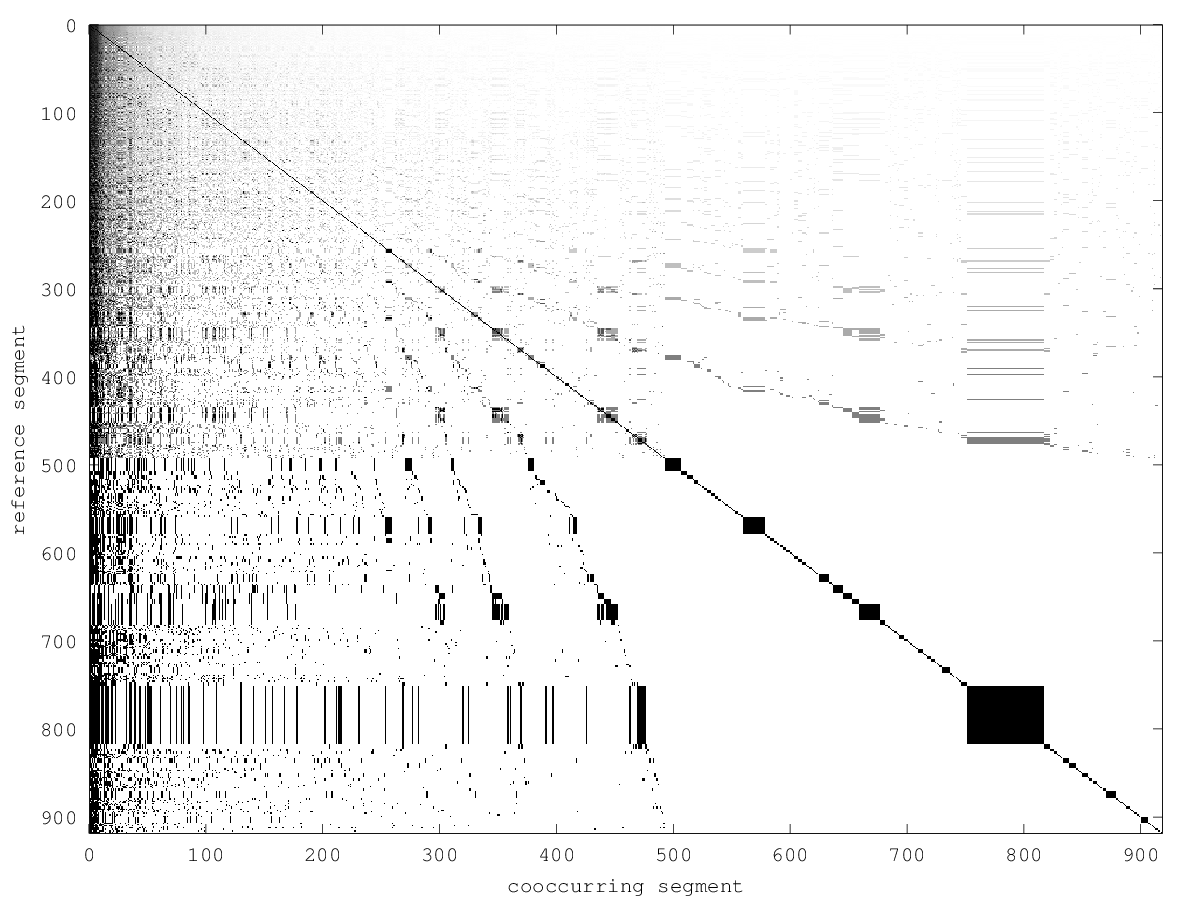
\includegraphics[width=0.75\textwidth]{imagespresentation/cooccurrence_matrix_upsid.png}
  \caption{Number of cooccurring phones for each phone in UPSID. The ordered by frequency of occurrence in languages.}
  \label{fig:cooccurrence_matrix_upsid}
  \end{figure}
}
\note{
For each phone we listed the cooccurring ones and the number of times they cooccur (how many languages). 
We normalize by the number of languages in which the reference phone occurs.
Observe that the most frequent phones in the database (left side) have a higher cooccurrence rate.
}



\frame
{
  \frametitle{Cooccurrence for a given phone}
  \vspace{-0.5cm}
  \begin{figure}[h!]
  \centering
  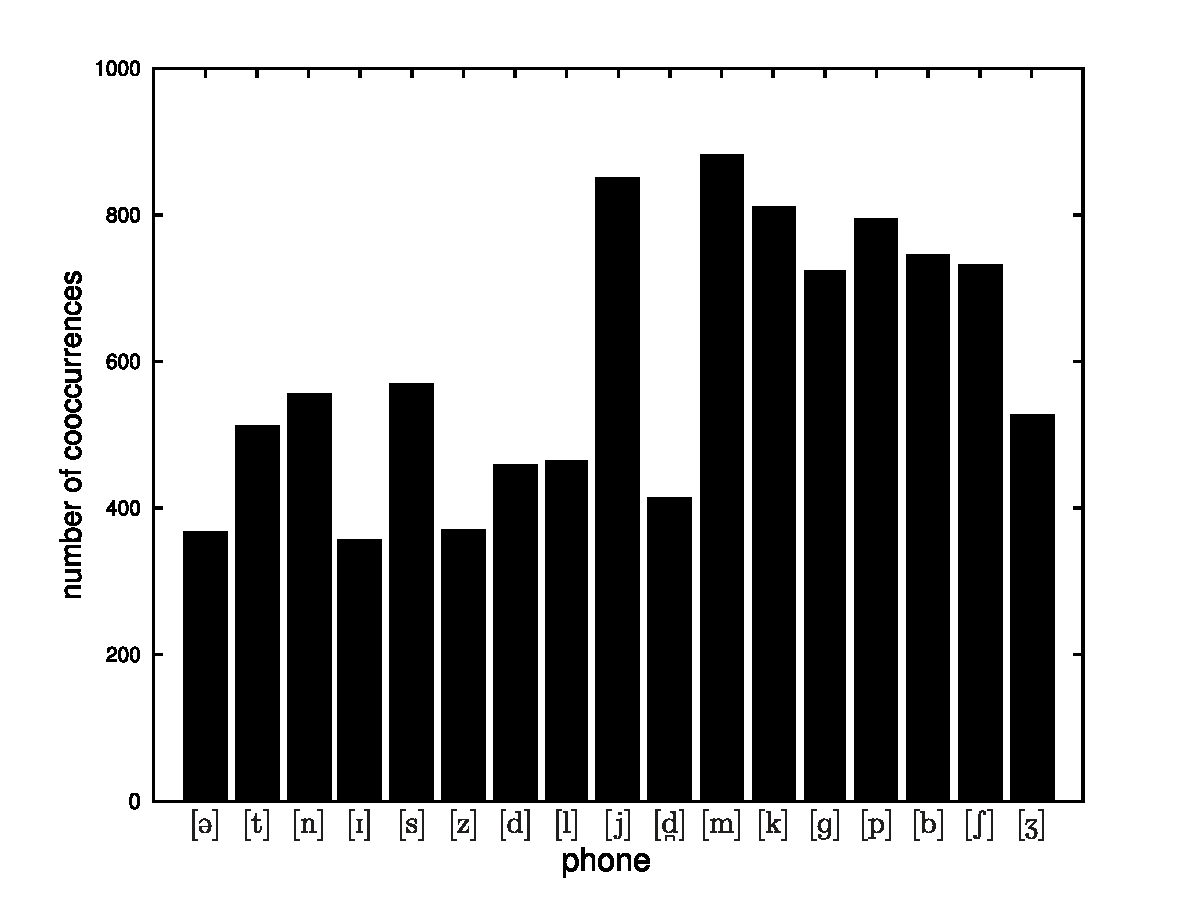
\includegraphics[width=0.9\textwidth]{images/num_cooccurring_phones.pdf}
  %\caption{The percentage of cooccurring phones among 919 speech sounds in UPSID.}
  \label{fig:numper_cooccurring_phones}
  \end{figure} 
}


\frame
{
  \frametitle{Cooccurrence: most frequent vs least frequent}
  \vspace{-0.5cm}
  \begin{figure}[h!]
  \centering
  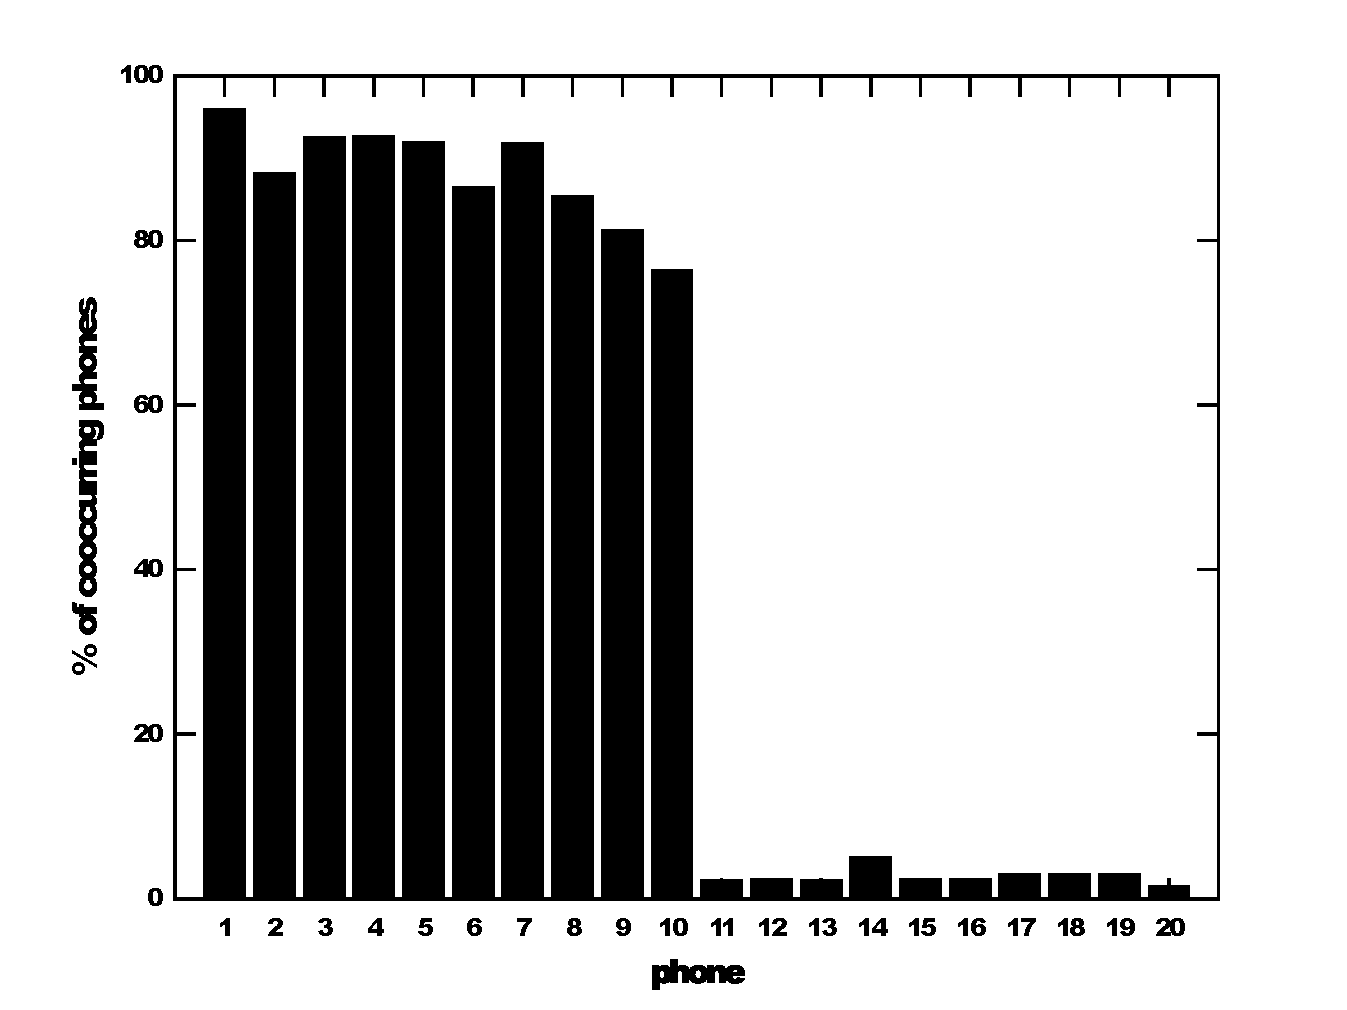
\includegraphics[width=0.8\textwidth]{images/numper_cooccurring_phones_10.pdf}
  %\caption{The percentage of cooccurring phones among 919 speech sounds in UPSID.}
  \label{fig:numper_cooccurring_phones_10}
  \end{figure} 
}

\frame
{
  \frametitle{Cooccurrence : languages and segments}
  \vspace{-0.3cm}
  \begin{figure}[h!]
  \centering
  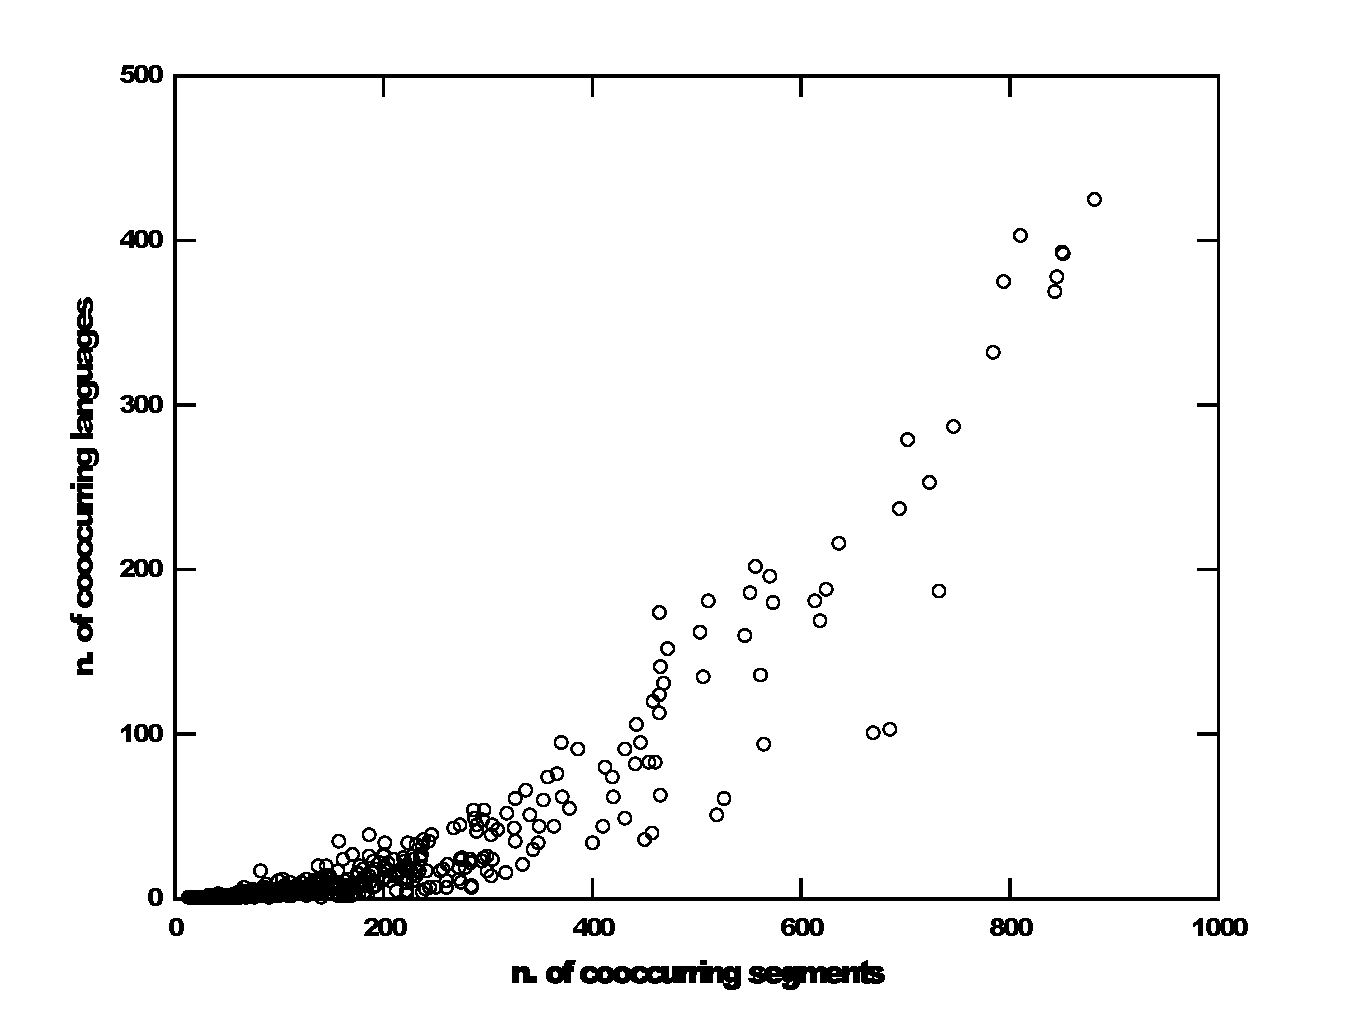
\includegraphics[width=0.8\textwidth]{images/coocc_of_speech_sounds.pdf}
  %\caption{Number of cooccurring languages and number of cooccurring phones for each phone.}
  \label{fig:coocc_of_speech_sounds}
  \end{figure} 
}


\frame
{
  \frametitle{Cooccurrence : languages and segments - German}
  \vspace{-0.3cm}
  \begin{figure}[h!]
  \centering
  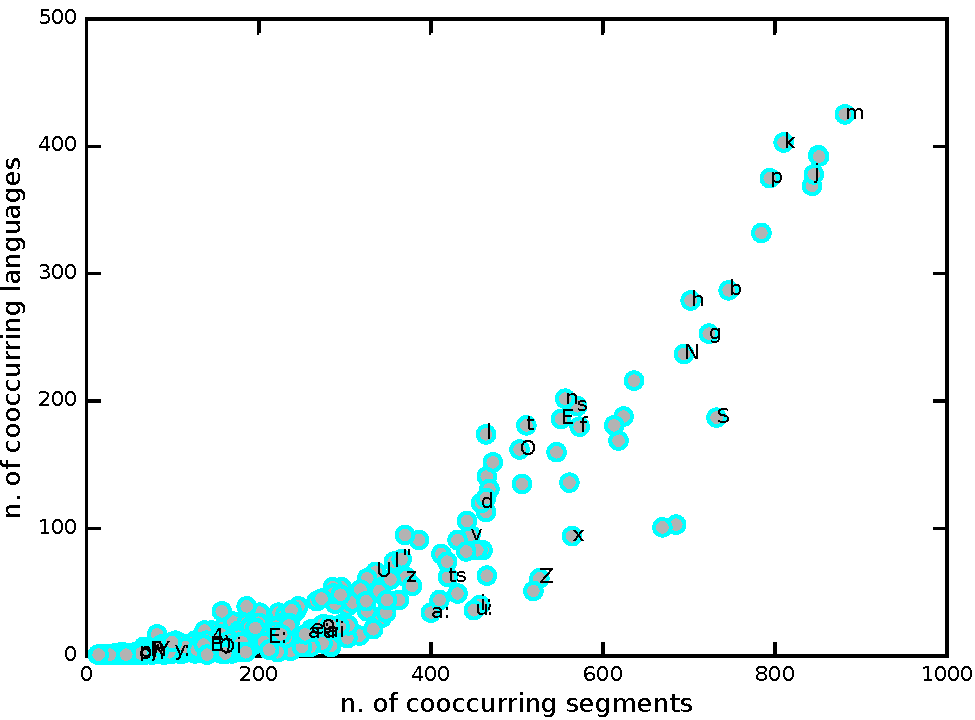
\includegraphics[width=0.8\textwidth]{images/coocc_of_speech_sounds_german.pdf}
  %\caption{Number of cooccurring languages and number of cooccurring phones for each phone.}
  \label{fig:coocc_of_speech_sounds_german}
  \end{figure}
}


\frame
{
  \frametitle{Cooccurrence : languages and segments - French}
  \vspace{-0.3cm}
  \begin{figure}[h!]
  \centering
  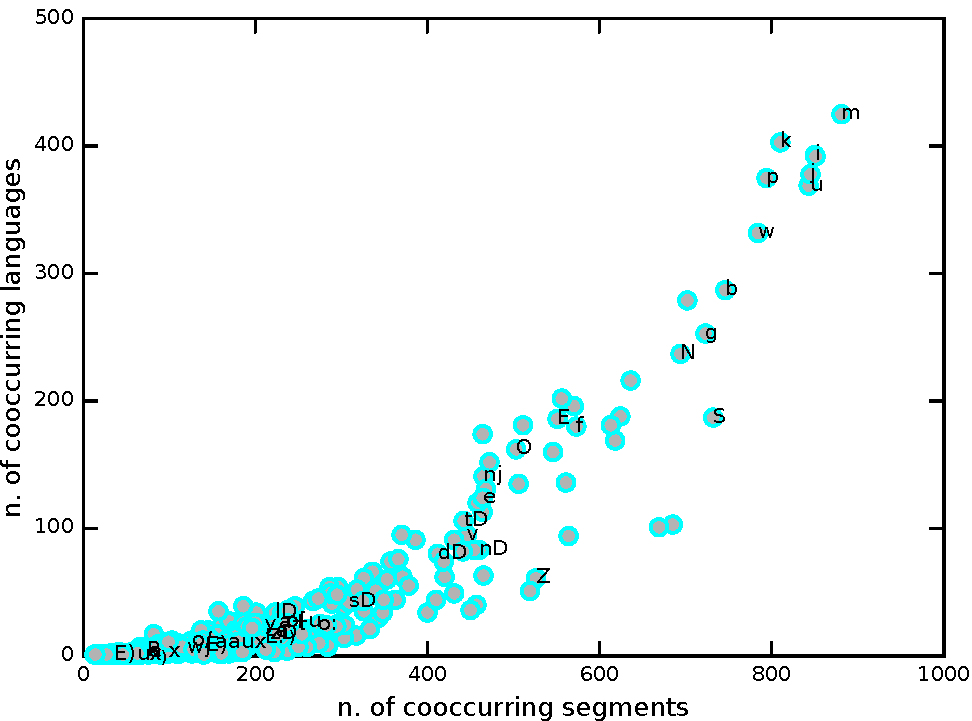
\includegraphics[width=0.8\textwidth]{images/coocc_of_speech_sounds_french.pdf}
  %\caption{Number of cooccurring languages and number of cooccurring phones for each phone.}
  \label{fig:coocc_of_speech_sounds_french}
  \end{figure}
}



\section{Intralanguage Statistical Analysis}

\frame
{
  \frametitle{Approach}
  \begin{itemize}
  \item synchrony 
  \item written corpus
  \item pronouncing dictionary
  \item statistical analysis
  \end{itemize}
}
\note{
Although ``languages are simultaneously products of history and entities existing at particular times''\citep{good2008} and both diachrony and synchrony aspects are important to determine what languages are, we focus here only on the synchrony aspects.

To carry out the analysis of it, we use large text databases, because it is much easier to be acquired, stored and handled.

A pronouncing dictionary is used to convert text into phones.

It is possible then to derive statistical analysis on this new database which statistically resembles a speech database.
}


\subsection{Text Database}
\frame
{
  \frametitle{Text Database}
  
  \begin{description}
  \item[Project Gutenberg] is a volunteer effort to provide free dgital access to cultural works. 
  It was founded by Michael S. Hart in 1971 and is the oldest digital library. 
  Most of its items are public domain books. Project Gutenberg claimed over 42,000 
  items in its collection (March 2013) \citep{projectgutenberg}.
  
  \item[Google Ngram] is a large database of n-grams (words combinations) based originally on 5.2 million books, 
  published between 1500 and 2008, containing 500 billion words in American English, British English, French, German,
  Spanish, Russian, or Chinese \citep{michel2011}.
  \end{description}

  %\begin{columns}[c]
  %\column{0.3\textwidth}
  %\begin{figure}[h!]
  %\centering
  %
\includegraphics[width=0.9\textwidth]{images/project_gutenberg.jpg}
  %\caption{Project Gutenberg.}
  %\label{fig:infinitylibrary}
  %\end{figure} 

  %\column{0.7\textwidth}

  %\begin{figure}[h!]
  %\centering
  %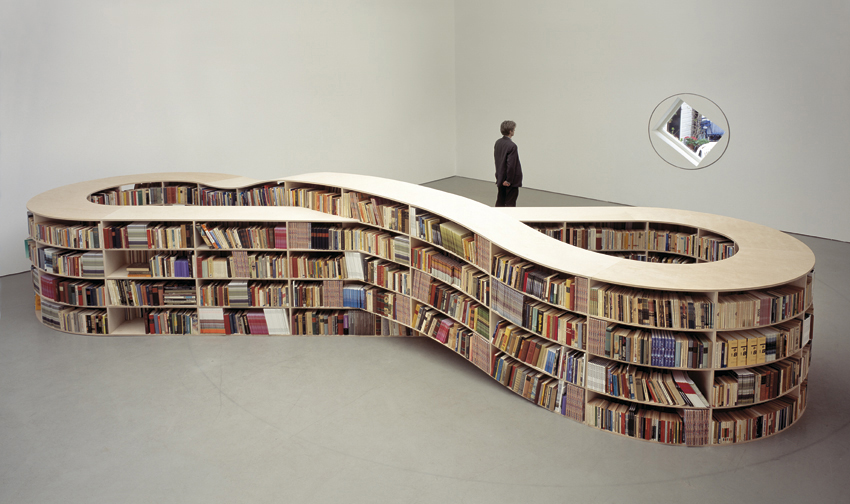
\includegraphics[width=0.9\textwidth]{images/infinitylibrary.jpg}
  %\caption{Large Database.}
  %\label{fig:infinitylibrary}
  %\end{figure} 
  
  %\end{columns}
}
\note{
Project Gutenberg is a volunteer effort to digitize and archive cultural works, to encourage the creation and distribution of eBooks. Founded in 1971 by Michael S. Hart, it is the oldest digital library. Most of the items in its collection are the full texts of public domain books. The project tries to make these as free as possible, in long-lasting, open formats that can be used on almost any computer. As of December 2009, Project Gutenberg claimed over 33,000 items in its collection. 


Today it is viable to have large databases and it is relatively easy do complile such databases and manage them.
That could not be dreamt a few years ago. It would be extremily good to have large speech databases in order to
study language as a spoken phenomena, investigate its usage and change, but it is
a much harder task to acchieve this goal.


reCAPTCHA is a user-dialogue system originally developed by Luis von Ahn, Ben Maurer, Colin McMillen, David Abraham and Manuel Blum at Carnegie Mellon University's main Pittsburgh campus, and acquired by Google in September 2009.
}


\subsection{Pronouncing Dictionary}
\frame
{
  \frametitle{Pronouncing Dictionary}
  
  \begin{description}
  \item[Dictionary] : Carnegie Mellon University Pronouncing Dictionary - is a machine-readable pronunciation dictionary for North American English that contains over 125,000 words and their transcriptions \citep{cmu2008}.
  \item[Phoneme set] : 39 phonemes.
  \item[Symbols] : ARPAbet.
  \end{description}

  \begin{tabular}{|c|c|c|c|c|}
\hline  Phoneme & IPA & Example & Translation & IPA Translation\\ 
\hline  AE & \textipa{[\ae]} & at & AE T & \textipa{[\ae t]} \\ 
\hline  B & \textipa{[b]} & be & B IY & \textipa{[bi]} \\ 
\hline  S & \textipa{[s]} & sea & S IY & \textipa{[si]} \\
\hline 
\end{tabular} 
}
\note{
To carry out the statistical analysis of a spoken language, we assume that a written language
presents a very similar characteristics, and then the statistical analysis using a written
text database and a text-to-phone transcription would be quite reasonable.

Arpabet is a phonetic transcription code developed by Advanced Research Projects Agency (ARPA) as a part of their Speech Understanding Project (1971-1976). It represents each phoneme of General American English with a distinct sequence of ASCII characters. Arpabet has been used in several speech synthesizers, including Computalker for the S-100 (Altair) system, SAM for the Commodore 64, SAY for the Amiga and TextAssist for the PC and Speakeasy from Intelligent Artefacts (see ST\_Robotics) which used the Votrax SC01 speech synthesiser IC. It is also used in the CMU Pronouncing Dictionary.
}



\subsection{Quantitative Analysis}
\frame
{
  \frametitle{Words Frequency}
\begin{tiny}
\begin{multicols}{4}
\begin{enumerate}
    \item the : 775911
	\item and : 471916
	\item of : 414499
	\item to : 350613
	\item a : 277321
	\item in : 226505
	\item i : 200689
	\item that : 173083
	\item he : 162183
	\item it : 145364
	\item was : 130804
	\item his : 129300
	\item you : 118473
	\item with : 114122
	\item is : 112640
	\item for : 107245
	\item as : 102009
	\item not : 96636
	\item be : 86896
	\item but : 81643
	\item had : 80327
	\item at : 76688
	\item her : 75761
	\item on : 75493
	\item my : 73879
	\item him : 72258
	\item have : 68463
	\item this : 67572
	\item all : 65960
	\item me : 64560
	\item by : 63944
	\item which : 63051
	\item she : 57839
	\item they : 57770
	\item from : 56128
	\item or : 52089
	\item so : 51617
	\item said : 50040
	\item no : 48930
	\item are : 45831
	\item one : 43822
	\item what : 41575
	\item them : 41320
	\item were : 40475
	\item will : 39733
	\item if : 38421
	\item there : 38209
	\item we : 37944
	\item when : 37385
	\item their : 36721
	\item who : 36109
	\item an : 35485
	\item your : 33401
	\item would : 32582
	\item do : 31225
	\item out : 30165
	\item then : 29682
	\item been : 29502
	\item up : 28860
	\item[] $\ldots$
\end{enumerate}
\end{multicols}
\end{tiny}
}


\frame
{
  \frametitle{Words Frequency and Zipf Law}
  \vspace{-0.25cm}
  \begin{figure}[h!]
  \centering
  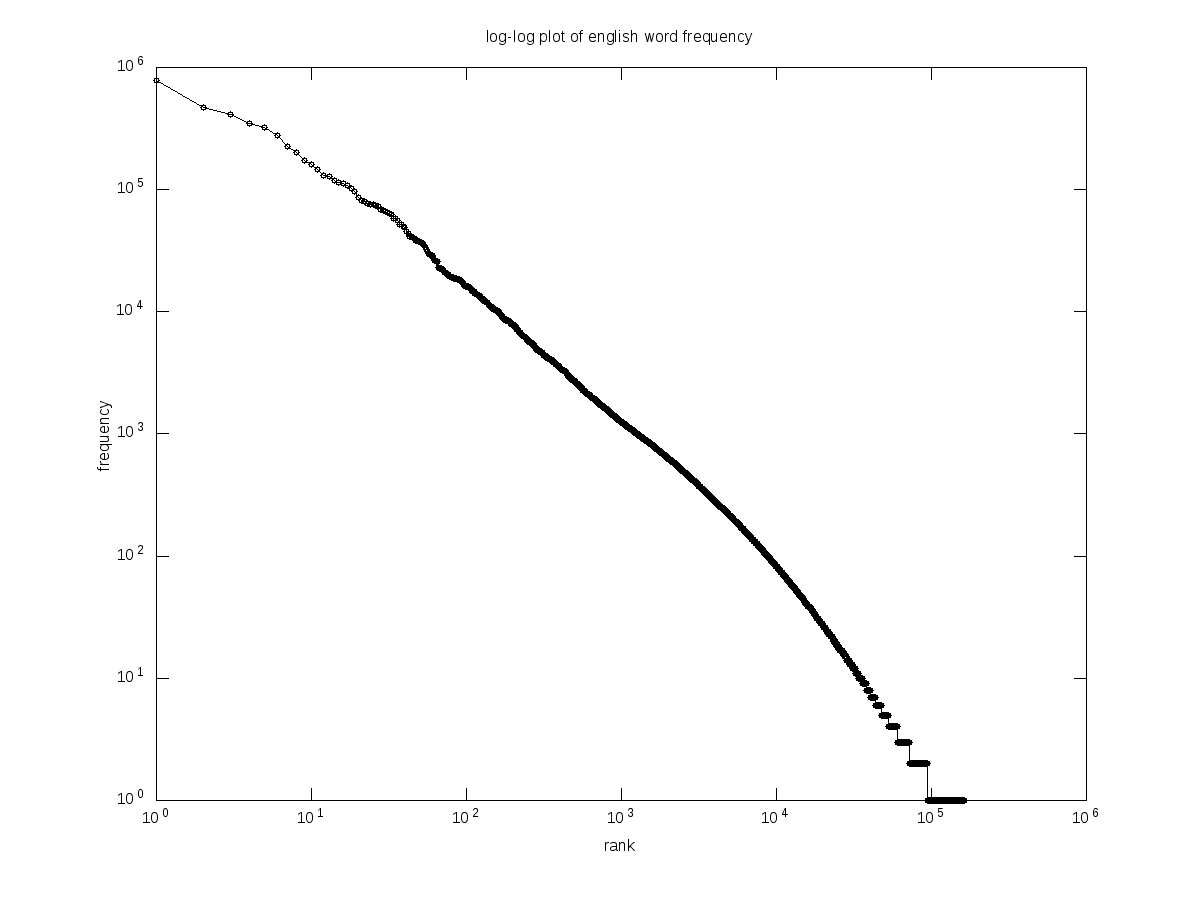
\includegraphics[width=0.8\textwidth]{images/wordfrequency_en.png}
  \vspace{-0.6cm}
  \caption{Log-log plot of words rank versus frequency of occurrence.}
  \label{fig:wordfrequency_en}
  \end{figure} 
}


\frame
{
  \frametitle{Letters Frequency}
  \begin{figure}[h!]
  \centering
  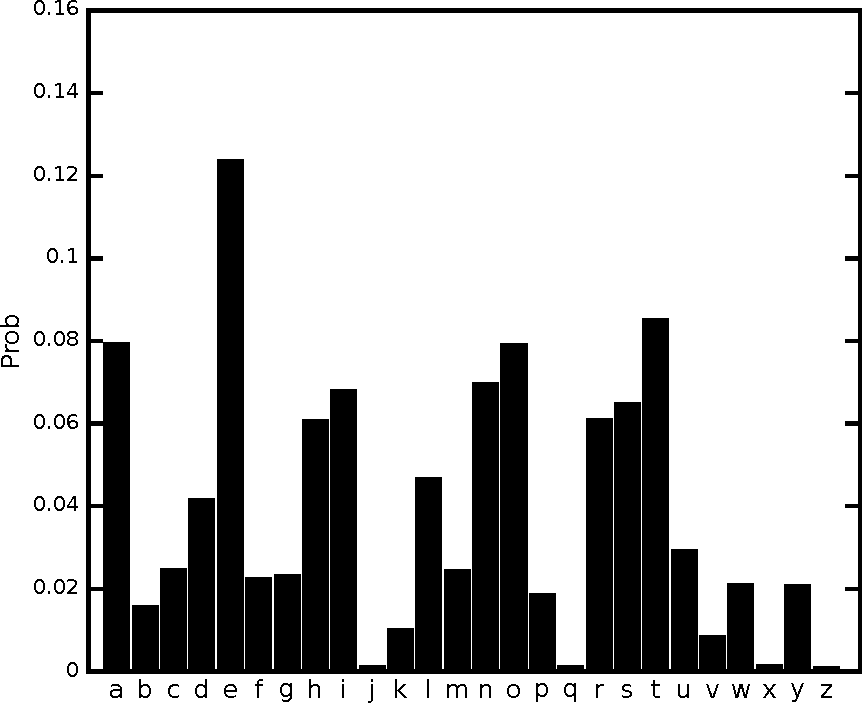
\includegraphics[width=0.7\textwidth]{images/ulysses_letters_prob_bargraph.pdf}
  \caption{Relative frequency of letters in text.}
  \label{fig:ulysses_letters_prob_bargraph}
  \end{figure} 
}


\frame
{
  \frametitle{Letters Frequency}
  \begin{figure}[h!]
  \makebox[\textwidth]{\parbox{1.5\textwidth}{ %
  \centering
  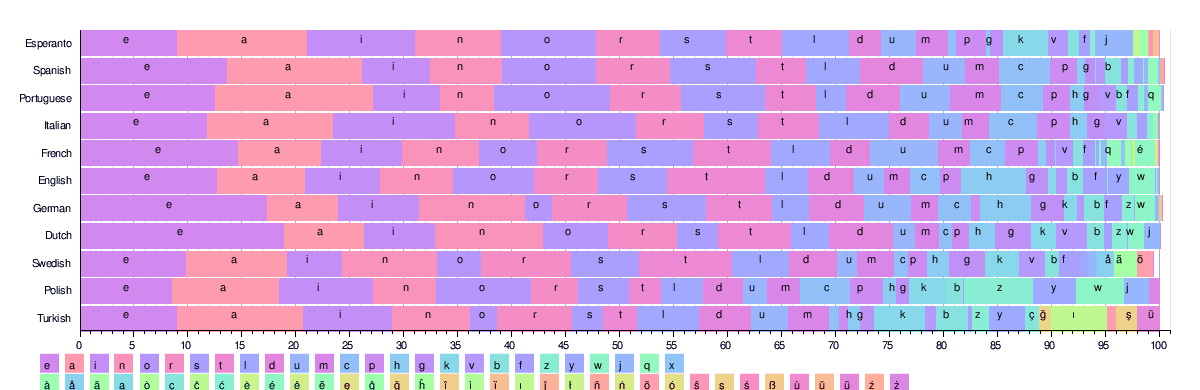
\includegraphics[width=1.2\textwidth]{imagespresentation/letters_freq.png}
  }}
  \caption{Frequency distributions of the 26 most common Latin letters across some languages (source: Wikipedia).}
  \label{fig:letters_freq}
  \end{figure} 
}


\frame
{
  \frametitle{Words Frequency - Transcribed}
\begin{tiny}
\begin{multicols}{4}
\begin{enumerate}
    \item DH AH : 775911
	\item AH N D : 471916
	\item AH V : 414499
	\item T UW : 350613
	\item AH : 277321
	\item IH N : 226505
	\item AY : 200689
	\item DH AE T : 173083
	\item HH IY : 162183
	\item IH T : 145364
	\item W AA Z : 130804
	\item HH IH Z : 129300
	\item Y UW : 118473
	\item W IH DH : 114122
	\item IH Z : 112640
	\item F AO R : 107245
	\item AE Z : 102009
	\item N AA T : 96636
	\item B IY : 86896
	\item B AH T : 81643
	\item HH AE D : 80327
	\item AE T : 76688
	\item HH ER : 75761
	\item AA N : 75493
	\item M AY : 73879
	\item HH IH M : 72258
	\item HH AE V : 68463
	\item DH IH S : 67572
	\item AO L : 65960
	\item M IY : 64560
	\item B AY : 63944
	\item W IH CH : 63051
	\item SH IY : 57839
	\item DH EY : 57770
	\item F R AH M : 56128
	\item AO R : 52089
	\item S OW : 51617
	\item S EH D : 50040
	\item N OW : 48930
	\item AA R : 45831
	\item W AH N : 43822
	\item W AH T : 41575
	\item DH EH M : 41320
	\item W ER : 40475
	\item W IH L : 39733
	\item IH F : 38421
	\item DH EH R : 38209
	\item W IY : 37944
	\item W EH N : 37385
	\item DH EH R : 36721
	\item HH UW : 36109
	\item AE N : 35485
	\item Y AO R : 33401
	\item W UH D : 32582
	\item D UW : 31225
	\item AO L AW T : 30165
	\item DH EH N : 29682
	\item B IH N : 29502
	\item AH P : 28860
	\item[] $\ldots$
\end{enumerate}
\end{multicols}
\end{tiny}
}









\frame
{
  \frametitle{Phones Frequency}
%\begin{tiny}
\begin{multicols}{4}
\begin{enumerate}
    \item \textipa{@} : 44539 
	\item \textipa{t} : 33131 
	\item \textipa{n} : 31928 
	\item \textipa{I} : 28845 
	\item \textipa{s} : 21928 
	\item \textipa{d} : 20032 
	\item \textipa{r} : 18563 
	\item \textipa{i} : 16482 
	\item \textipa{l} : 15816 
	\item \textipa{E} : 13896 
	\item \textipa{m} : 13072 
	\item \textipa{3\textrhoticity} : 12640 
	\item \textipa{k} : 12308 
	\item \textipa{w} : 11107 
	\item \textipa{z} : 10744 
	\item \textipa{D} : 10720 
	\item \textipa{v} : 10407 
	\item \textipa{h} : 10009 
	\item \textipa{f} : 9391 
	\item \textipa{A} : 8744 
	\item \textipa{\ae} : 8635 
	\item \textipa{b} : 8390 
	\item \textipa{u} : 7972 
	\item \textipa{p} : 7501 
	\item \textipa{O} : 7429 
	\item \textipa{eI} : 6196 
	\item \textipa{aI} : 6148 
	\item \textipa{oW} : 5283 
	\item \textipa{S} : 4915 
	\item \textipa{N} : 4861 
	\item \textipa{g} : 3351 
	\item \textipa{tS} : 2501 
	\item \textipa{j} : 2462 
	\item \textipa{T} : 2309 
	\item \textipa{U} : 2276 
	\item \textipa{aU} : 2242 
	\item \textipa{dZ} : 2100 
	\item \textipa{OI} : 326 
	\item \textipa{Z} : 314 
\end{enumerate}
\end{multicols}
%\end{tiny}
}


\frame
{
  \frametitle{Phones Frequency - Log-log plot}
\begin{figure}[h!]
\centering
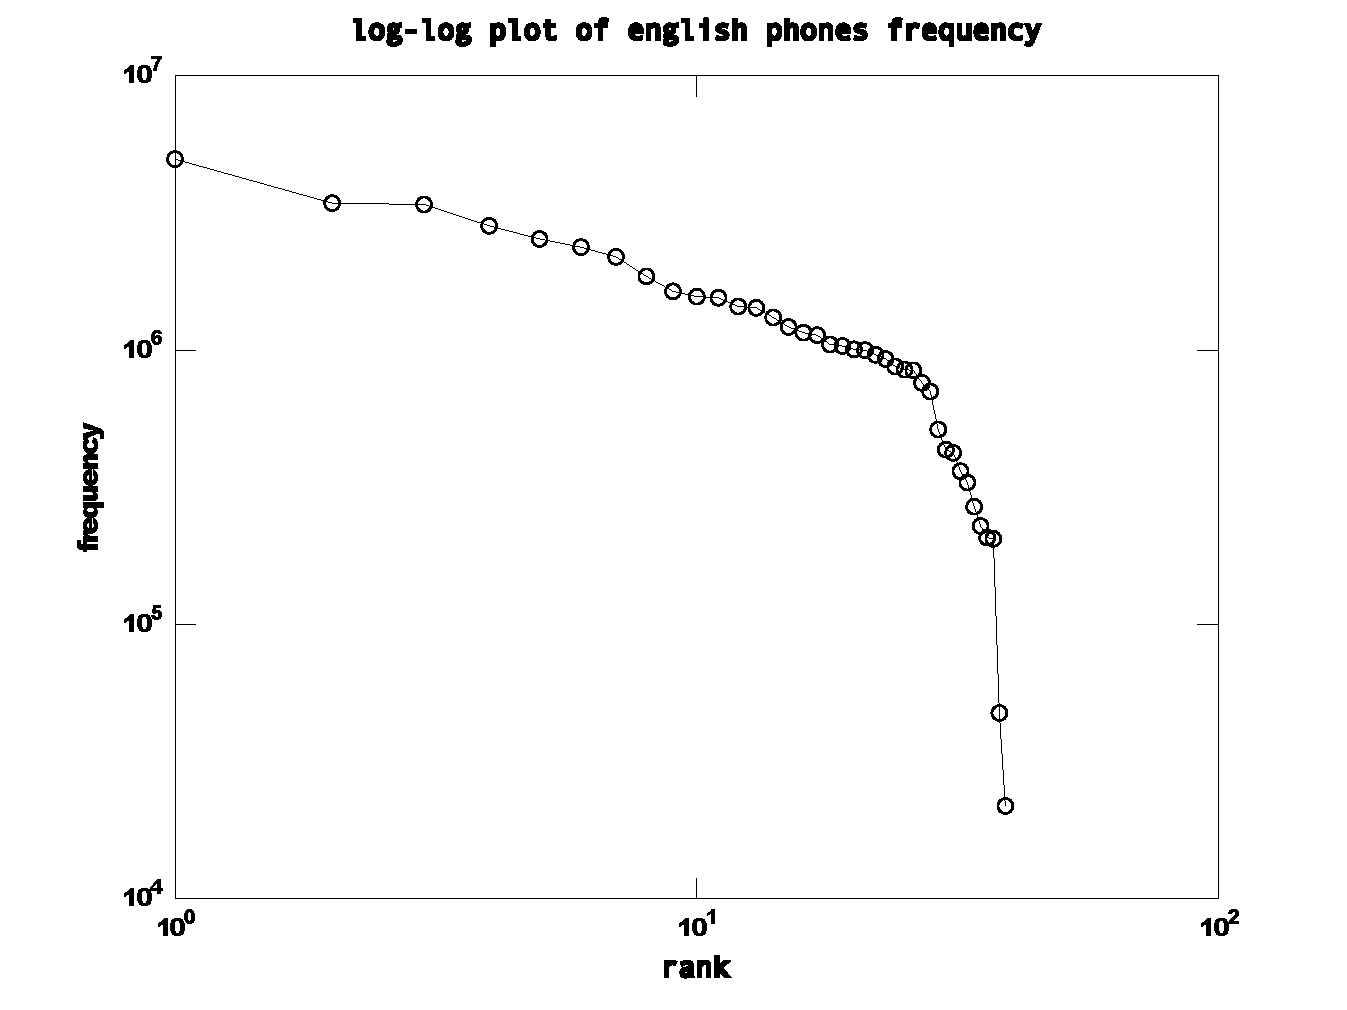
\includegraphics[width=0.7\textwidth]{images/phonesfrequency_en.pdf}
\caption{Log-log plot of phones rank versus frequency of occurrence.}
\label{fig:phonesfrequency_en}
\end{figure} 
}
\note{
This is not an example of distribution with large number of rare events ... where ``rare events are common''
We might say that there are no rare events. Zipf's law is found only on distributions with large number of rare events.

The simple ``maximum likelihood'' method for predicting estimate the probability of an event-type that has occurred 
$r$ times in $N$ trials as $r/N$. This generally works well if r is fairly large (and if the world doesn't change too much). 
But as $r$ gets smaller, the maximum likelihood estimate gets worse. And if $r$ is zero, it may still be quite unwise to bet 
that the event-type in question will never occur in the future. Even more important, the fraction of future events whose past 
counts are zero may be substantial.

One of the present time (2000) characteristics of the study of Zipf's law is the increase of interest in the more general 
concept of ``distributions with a large number of rare events'' (LNRE distributions), which was introduced and first 
systematically studied by \citep{khmaladze1987}.
}



\frame
{
  \frametitle{Probability of occurrence of \textipa{[@]} across words rank}
\begin{figure}[h!]
\centering
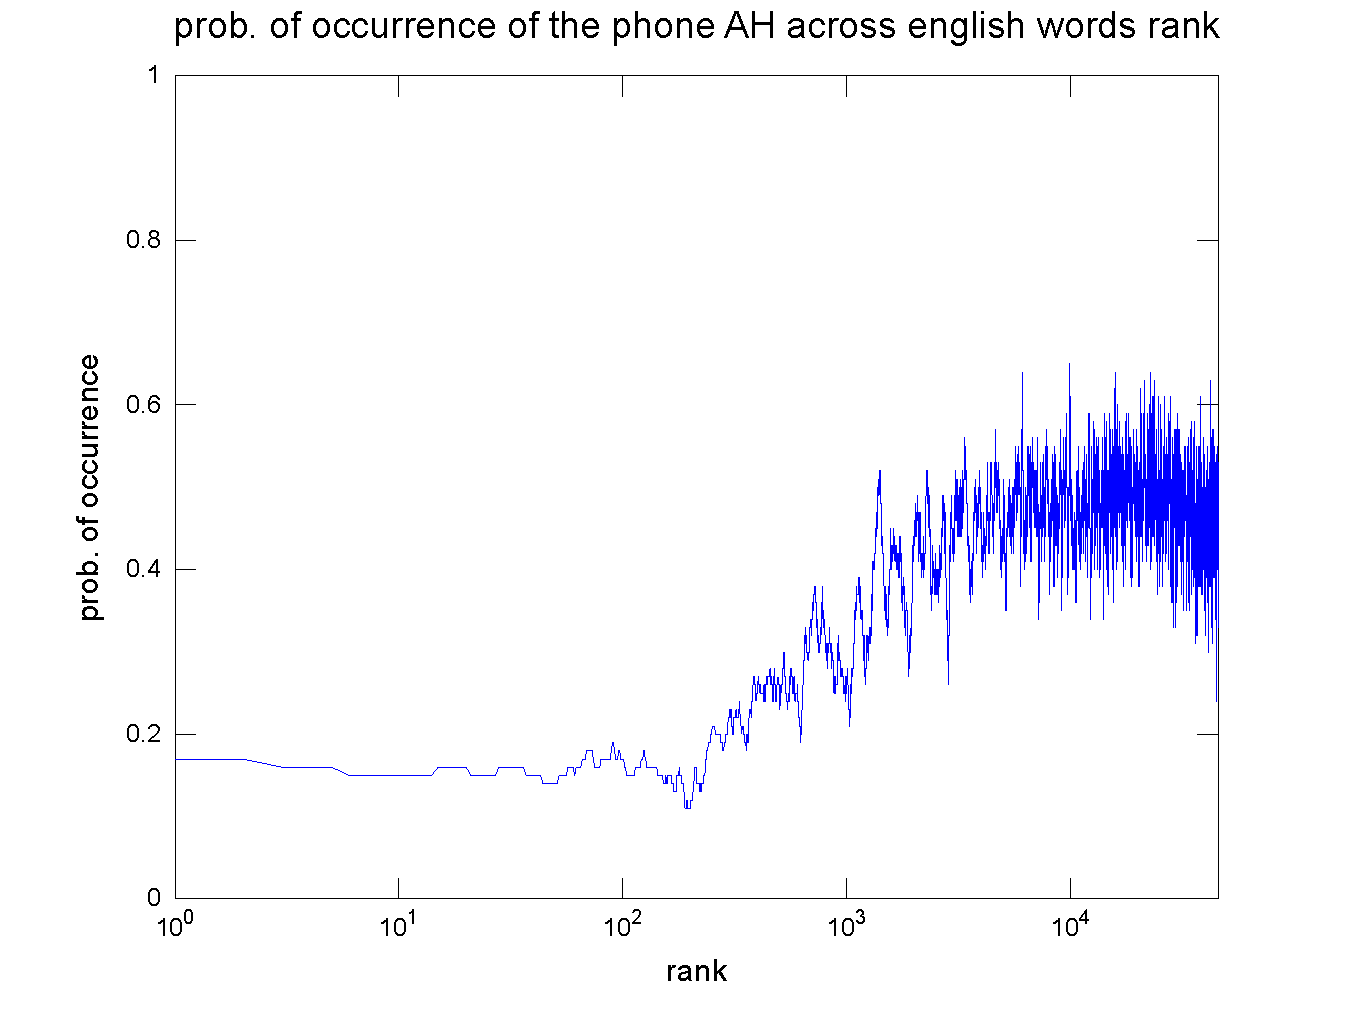
\includegraphics[width=0.7\textwidth]{images/proboccwordsphone_AH.pdf}
\caption{Probability of occurrence of \textipa{[@]} in words versus words rank.}
\label{fig:proboccwordsphone_AH}
\end{figure} 
}
\note{
We might wonder whether some phones are more frequent then others because they are present in most frequent words, what would lead them along to a higher frequency of occurrence. The present graphic and the following ones shows this is a false hypothesis.
}


\frame
{
  \frametitle{Probability of occurrence of \textipa{[t]} across words rank}
\begin{figure}[h!]
\centering
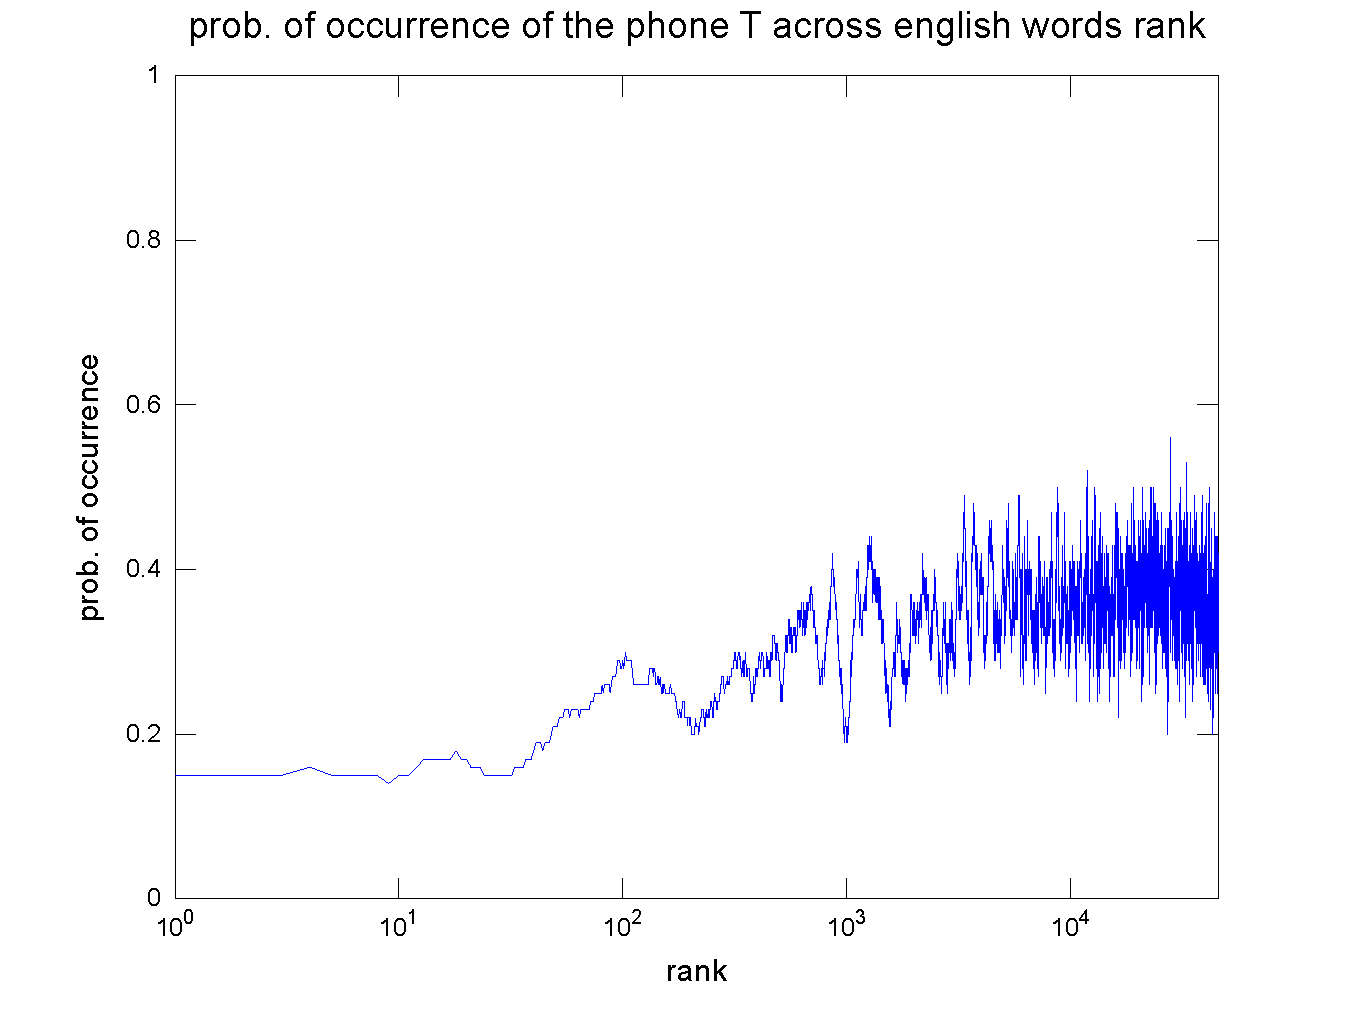
\includegraphics[width=0.7\textwidth]{images/proboccwordsphone_T.pdf}
\caption{Probability of occurrence of \textipa{[t]} in words versus words rank.}
\label{fig:proboccwordsphone_T}
\end{figure} 
}


\frame
{
  \frametitle{Probability of occurrence of \textipa{[n]} across words rank}
\begin{figure}[h!]
\centering
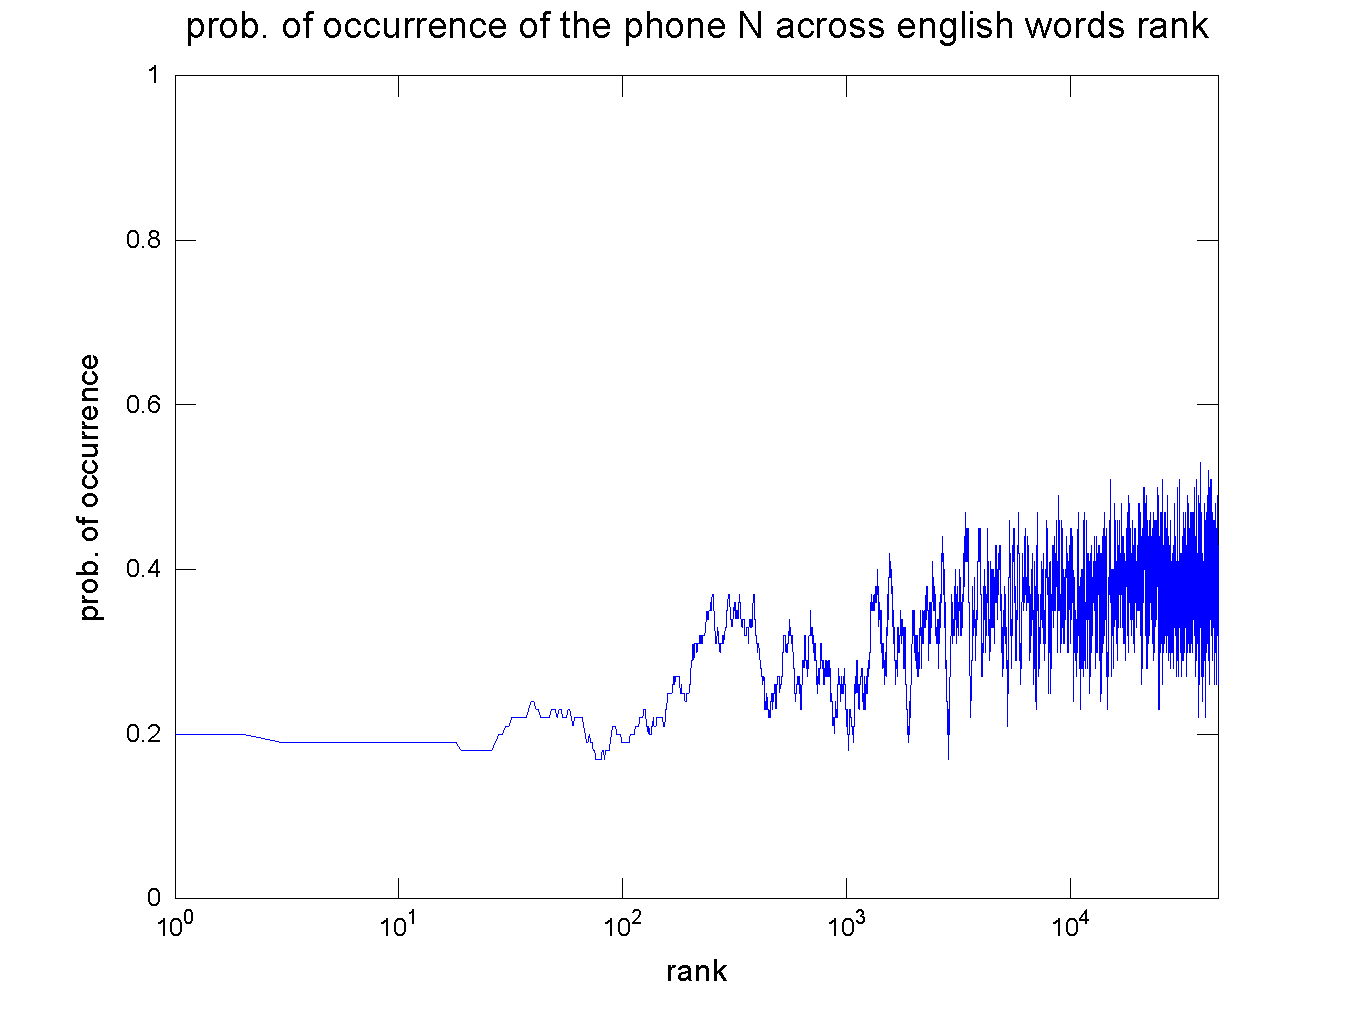
\includegraphics[width=0.7\textwidth]{images/proboccwordsphone_N.pdf}
\caption{Probability of occurrence of \textipa{[n]} in words versus words rank.}
\label{fig:proboccwordsphone_N}
\end{figure} 
}


\frame
{
  \frametitle{Probability of occurrence of \textipa{[U]} across words rank}
\begin{figure}[h!]
\centering
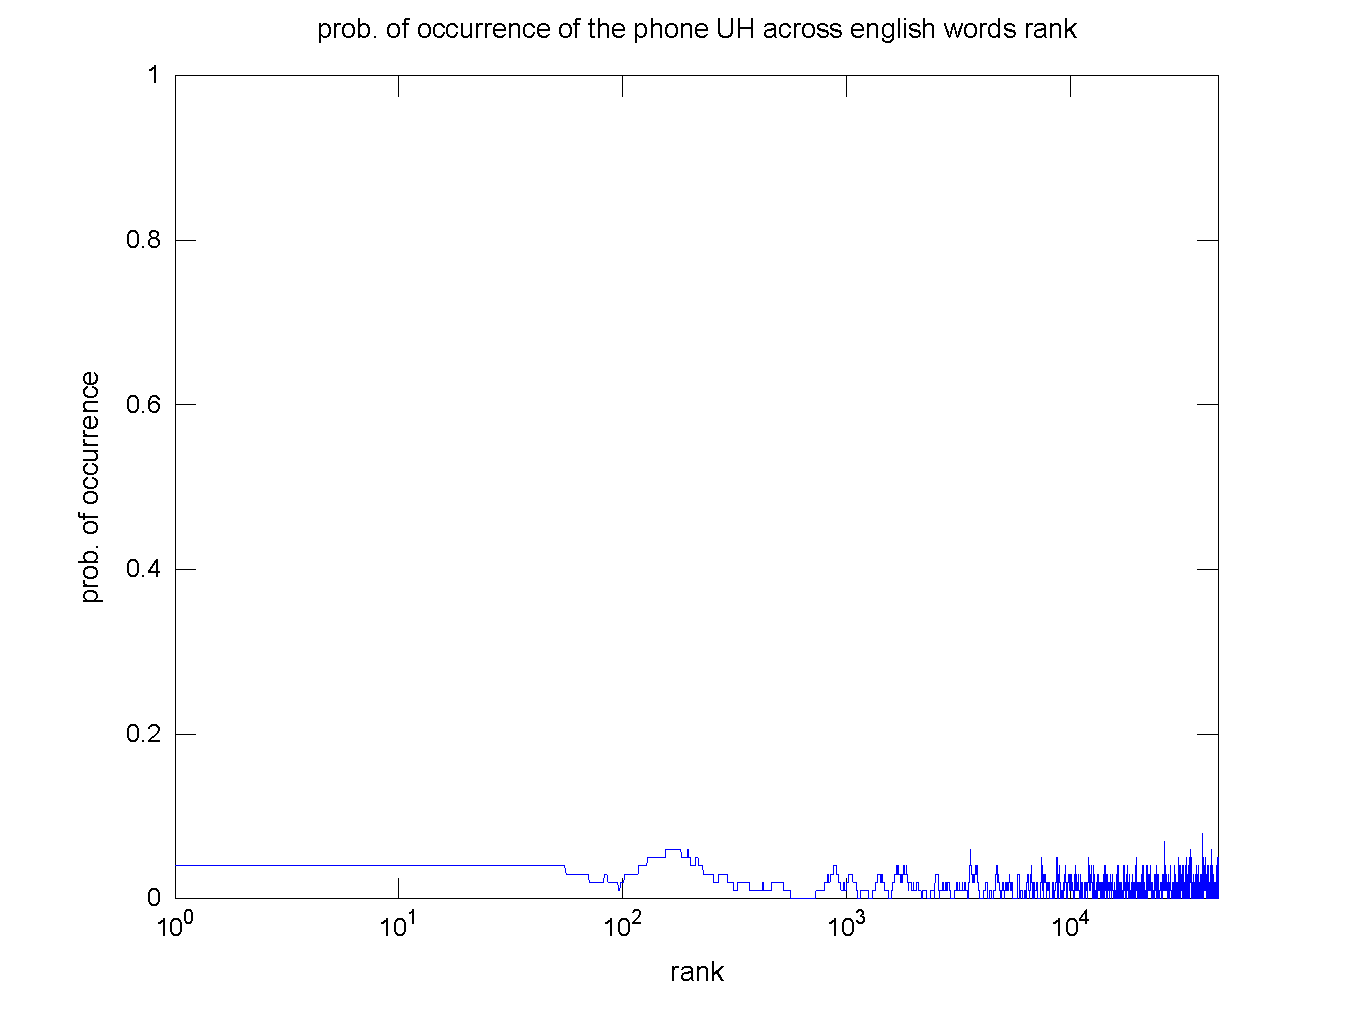
\includegraphics[width=0.7\textwidth]{images/proboccwordsphone_UH.pdf}
\caption{Probability of occurrence of \textipa{[U]} in words versus words rank.}
\label{fig:proboccwordsphone_UH}
\end{figure} 
}


\frame
{
  \frametitle{Probability of occurrence of \textipa{[OI]} across words rank}
\begin{figure}[h!]
\centering
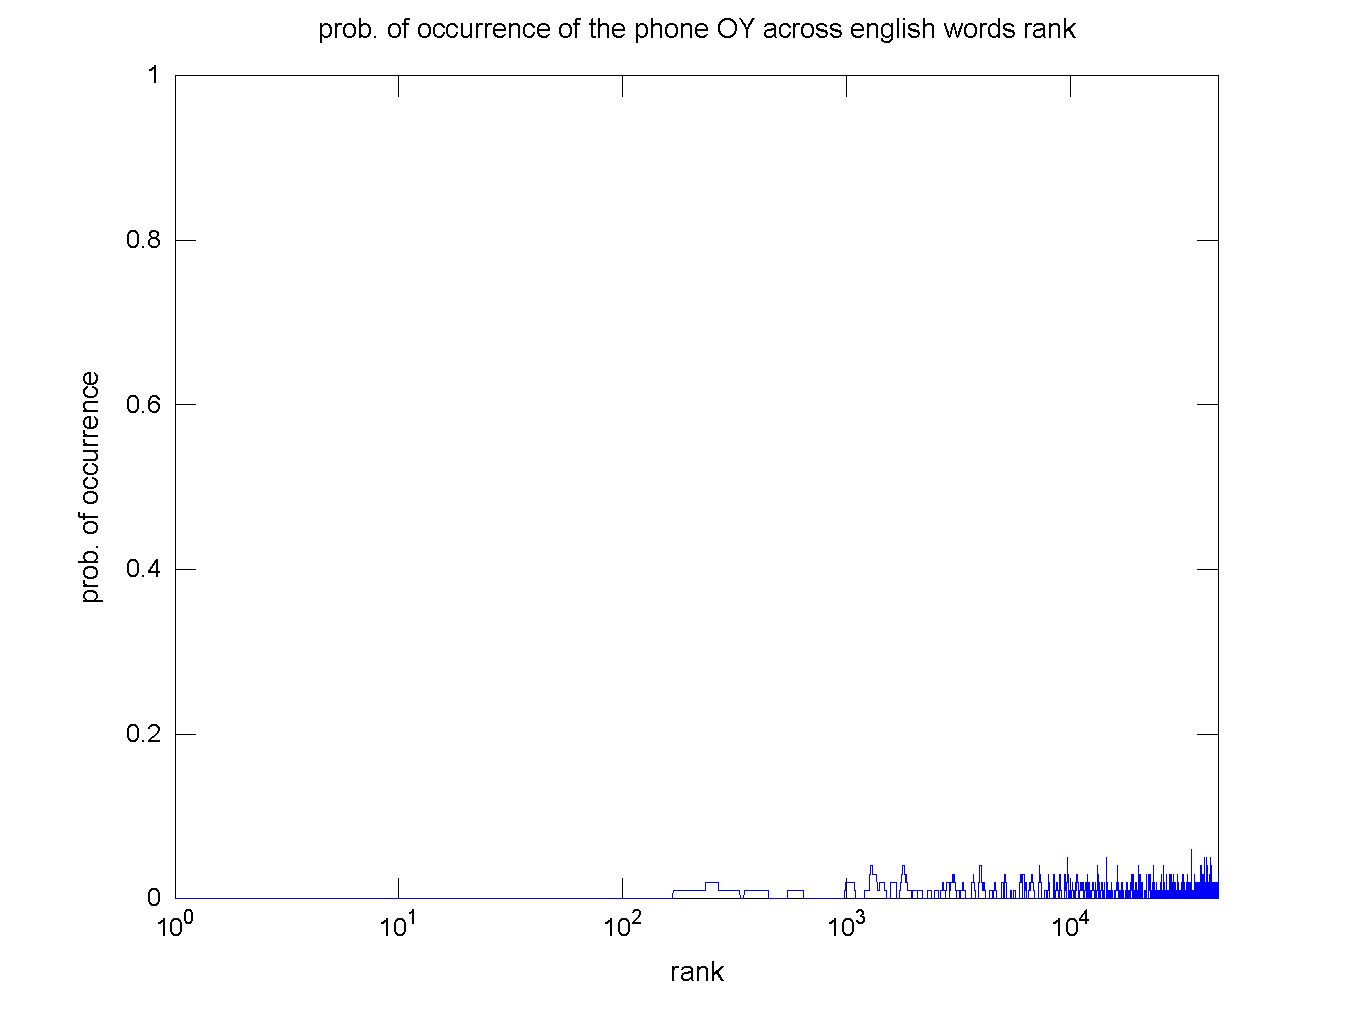
\includegraphics[width=0.7\textwidth]{images/proboccwordsphone_OY.pdf}
\caption{Probability of occurrence of \textipa{[OI]} in words versus words rank.}
\label{fig:proboccwordsphone_OY}
\end{figure} 
}


\frame
{
  \frametitle{Probability of occurrence of \textipa{[Z]} across words rank}
\begin{figure}[h!]
\centering
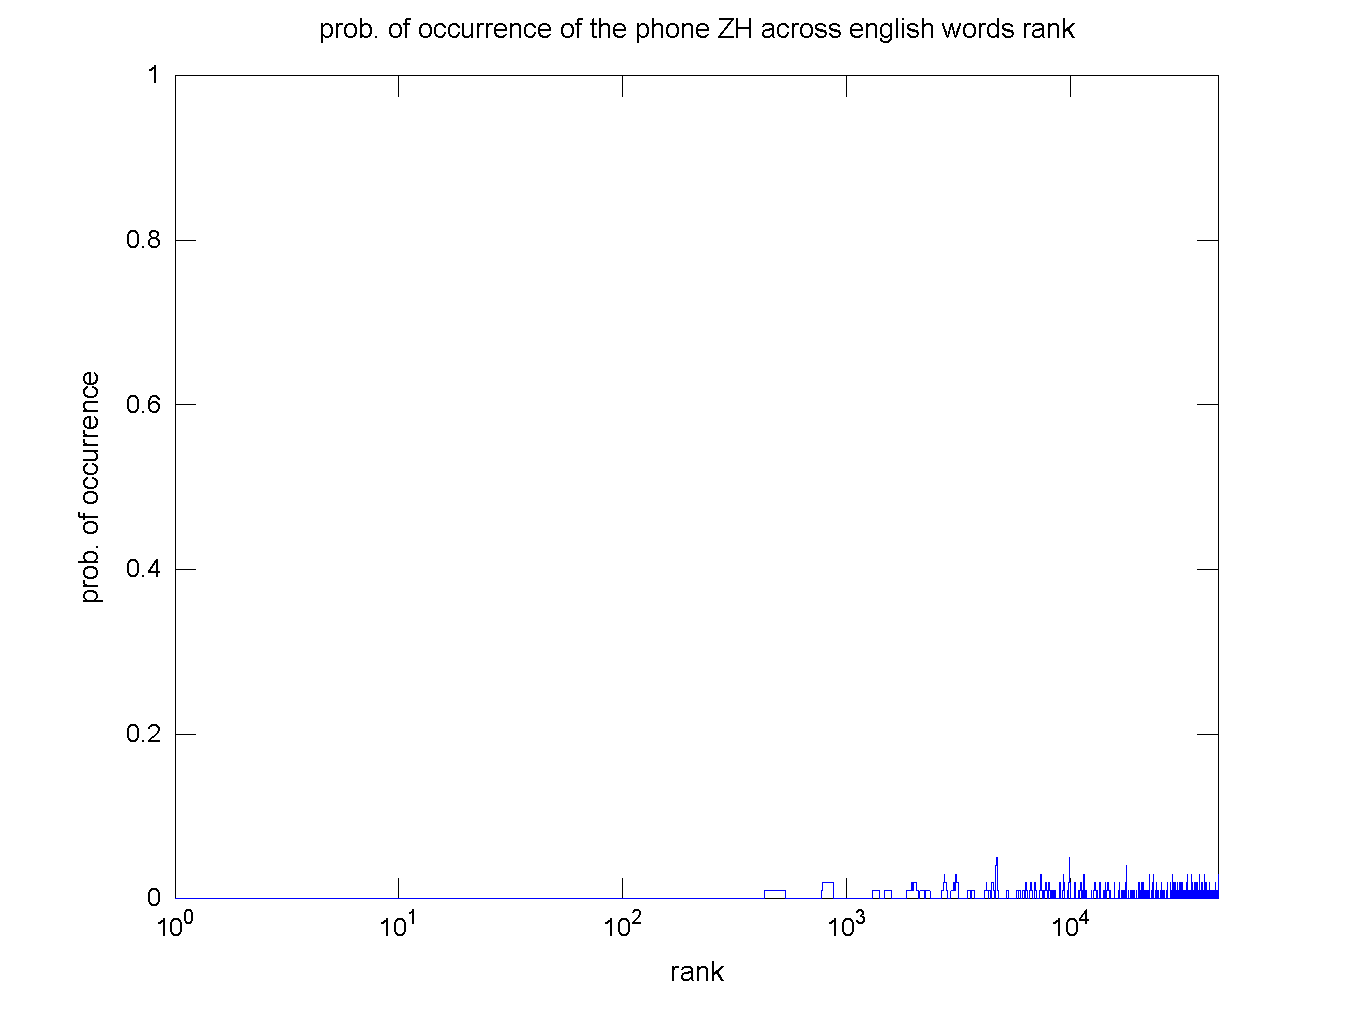
\includegraphics[width=0.7\textwidth]{images/proboccwordsphone_ZH.pdf}
\caption{Probability of occurrence of \textipa{[Z]} in words versus words rank.}
\label{fig:proboccwordsphone_ZH}
\end{figure} 
}


\frame
{
  \frametitle{Diphones : Frequency of occurrence}

\begin{tiny}
\begin{multicols}{4}
\begin{enumerate}
    \item \textipa{@n} : 1296408
    \item \textipa{D@} : 785354
    \item \textipa{nd} : 784028
    \item \textipa{st} : 651129
    \item \textipa{@v} : 489267
    \item \textipa{Or} : 472069
    \item \textipa{In} : 470069
    \item \textipa{tu} : 425544
    \item \textipa{t@} : 420825
    \item \textipa{IN} : 387096
    \item \textipa{Iz} : 380357
    \item \textipa{@l} : 372847
    \item \textipa{En} : 349905
    \item \textipa{nt} : 337193
    \item \textipa{\ae t} : 284460
    \item \textipa{wI} : 282526
    \item \textipa{@t} : 265396
    \item \textipa{Er} : 264293
    \item \textipa{r@} : 261447
    \item \textipa{It} : 260544
    \item \textipa{@s} : 246996
    \item \textipa{ju} : 245715
    \item \textipa{h\ae} : 237724
    \item \textipa{hI} : 237490
    \item \textipa{@m} : 233793
    \item \textipa{ri} : 219997
    \item \textipa{li} : 219652
    \item \textipa{An} : 213755
    \item \textipa{\ae n} : 213169
    \item \textipa{s@} : 210385
    \item \textipa{Is} : 208619
    \item \textipa{D\ae} : 194602
    \item \textipa{@f} : 193570
    \item \textipa{Ar} : 193525
	\item[] $\vdots$
	\item[(1120)] \textipa{uaI} : 1
	\item[(1121)] \textipa{OIA} : 1
	\item[(1122)] \textipa{bS} : 1
	\item[(1123)] \textipa{pv} : 1
	\item[(1124)] \textipa{iU} : 1
	\item[(1125)] \textipa{EoU} : 1
\end{enumerate}
\end{multicols}
\end{tiny}
}



\frame
{
  \frametitle{Diphones Frequency - Log-log plot}
\begin{figure}[h!]
\centering
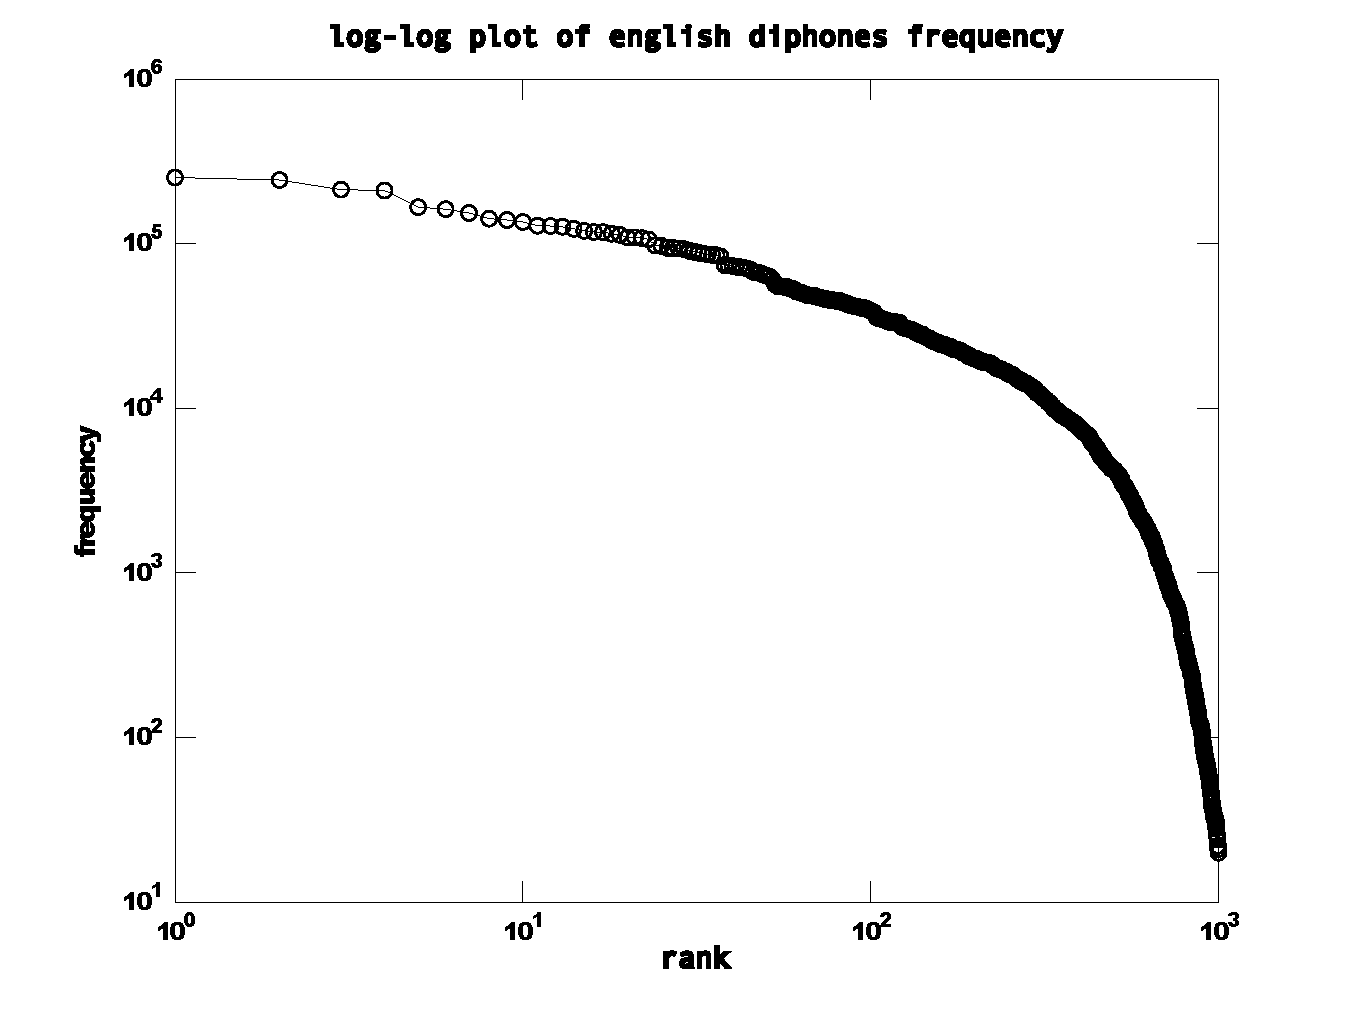
\includegraphics[width=0.7\textwidth]{images/diphonesfrequency_en.pdf}
\caption{Log-log plot of the diphones frequency of occurrence versus their rank.}
\label{fig:diphonesfrequency_en}
\end{figure} 
}


\frame
{
  \frametitle{Diphones : phone-normalized frequency of occurrence}
\begin{multicols}{6}
\begin{enumerate}
    \item \textipa{Z@}
    \item \textipa{D@}
    \item \textipa{@v}
    \item \textipa{S@} 
    \item \textipa{dZ@}
    \item \textipa{b@}
    \item \textipa{@l}
    \item \textipa{@f}
    \item \textipa{ju} 
    \item \textipa{@m}
    \item \textipa{Or}
    \item \textipa{@b}
    \item \textipa{@tS}
    \item \textipa{nd}
    \item \textipa{k@} 
    \item \textipa{@g}
    \item \textipa{@p}
    \item[] $\vdots$
	\item[(1120)] \textipa{zs}
	\item[(1121)] \textipa{uaI}
	\item[(1122)] \textipa{aIh}
	\item[(1123)] \textipa{EoU}
	\item[(1124)] \textipa{ddZ}
	\item[(1125)] \textipa{tv}
\end{enumerate}
\end{multicols}
}


\frame
{
  \frametitle{Diphones Normalized Frequency - Log-log plot}
\vspace{-0.2cm}
\begin{figure}[h!]
\centering
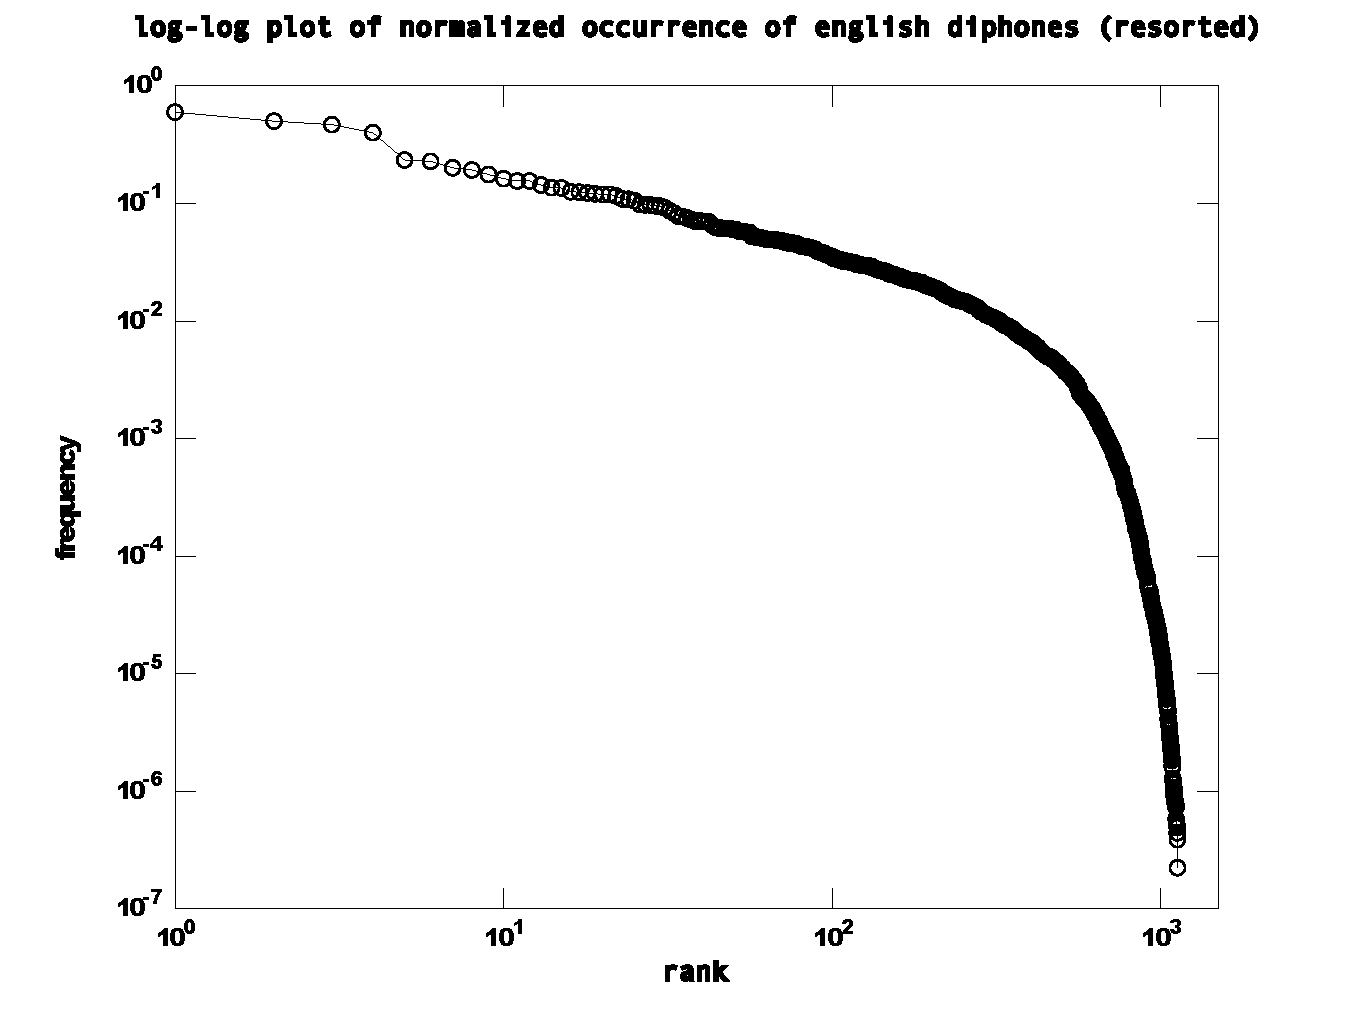
\includegraphics[width=0.7\textwidth]{images/diphonesnormalizedfrequencyresorted_en.pdf}
\vspace{-0.2cm}
\caption{\begin{scriptsize}Log-log plot of the diphones normalized frequency of occurrence versus their rank. The normalization is made using the frequency of occurrence of each phone in the pair.\end{scriptsize}}
\label{fig:diphonesnormalizedfrequencyresorted_en}
\end{figure} 
}  
\note{
the normalization is 
total number of diphones divided by the occurrence of either one of the phones in the diphone pair

% diphonesfreqnorm(k) = diphonesfreq(k)/(normF - diphonesfreq(k));

}


\frame
{
  \frametitle{Diphones Conditional Probability}
\vspace{-0.5cm}
\begin{figure}[h!]
\centering
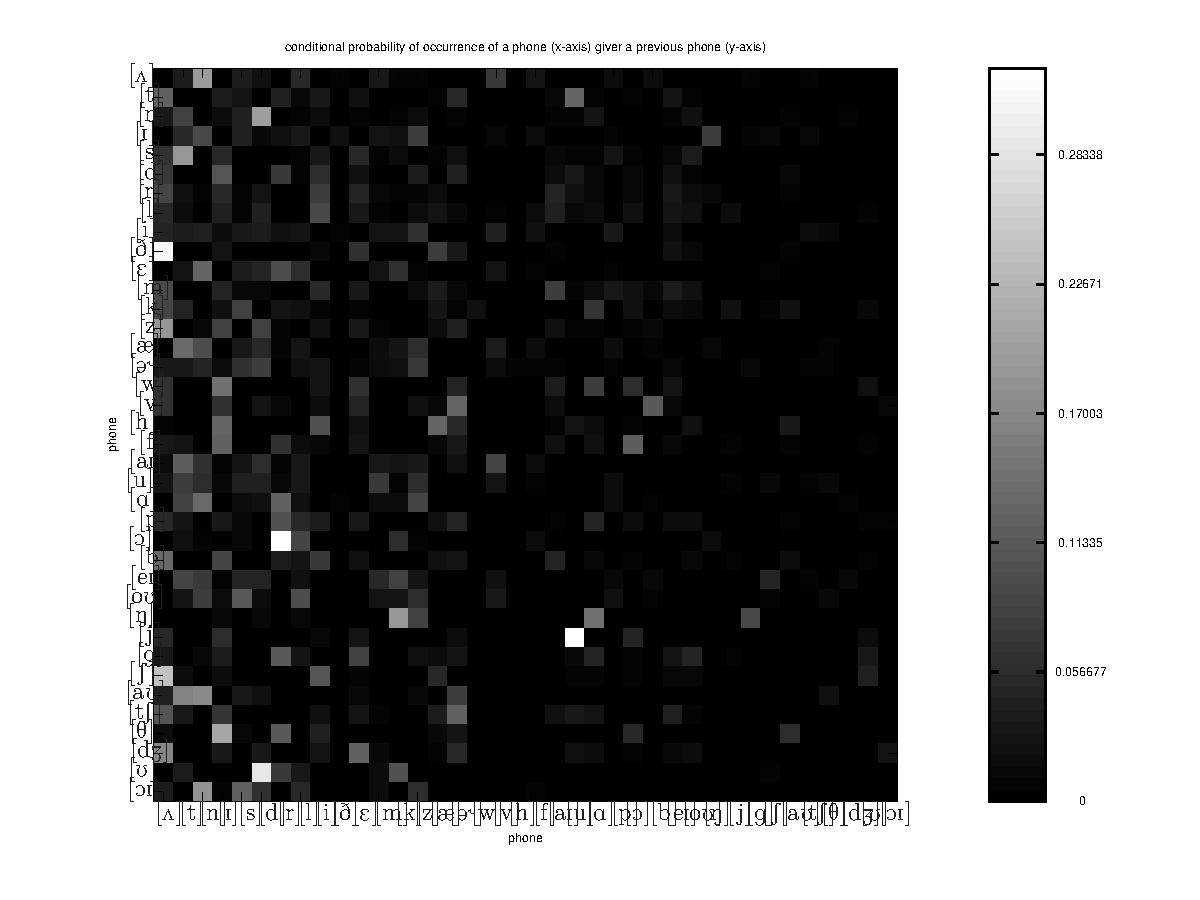
\includegraphics[width=0.85\textwidth]{images/diphones_cond_probability_en.pdf}
\vspace{-0.7cm}
\caption{Probability of occurrence of a phone given another previous phone.}
%(30,22) = \textipa{[j u]}, (25,7) = \textipa{[O r]}, (37,6) = \textipa{[U d]}, (10,1) = \textipa{[D @]}}
\label{fig:diphones_cond_probability_en}
\end{figure} 
}
\note{
We observe in the figure that the most
frequent phones (in the left part of the figure) also have an average higher conditional
probability of occurrence regardless which the prior phone is.


(30,22) = \textipa{[j u]}

(25,7) = \textipa{[O r]}

(37,6) = \textipa{[U d]}

(10,1) = \textipa{[D @]}
}





\frame
{
  \frametitle{Triphone Probabilities}
  \begin{figure}[h!]
  \centering
  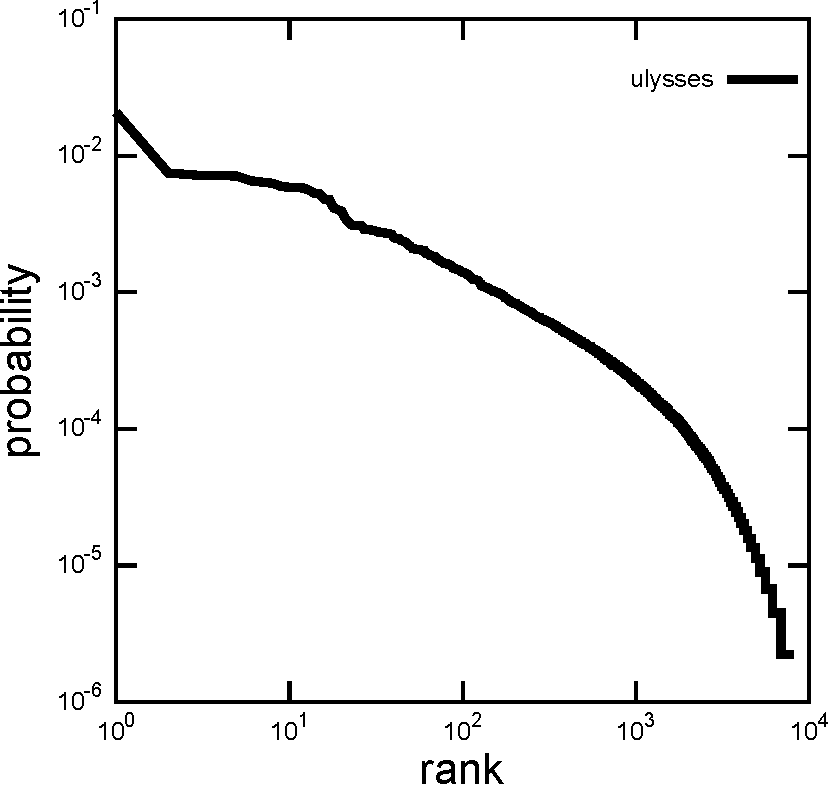
\includegraphics[width=0.6\textwidth]{imagespresentation/ulysses_triphones_probabilities.pdf}
  \caption{Triphone Probability (from \emph{Ulysses)}.}
  \label{fig:ulysses_triphones_probabilities}
  \end{figure} 
}


\frame
{
  \frametitle{Syllable Probabilities}
  \begin{figure}[h!]
  \centering
  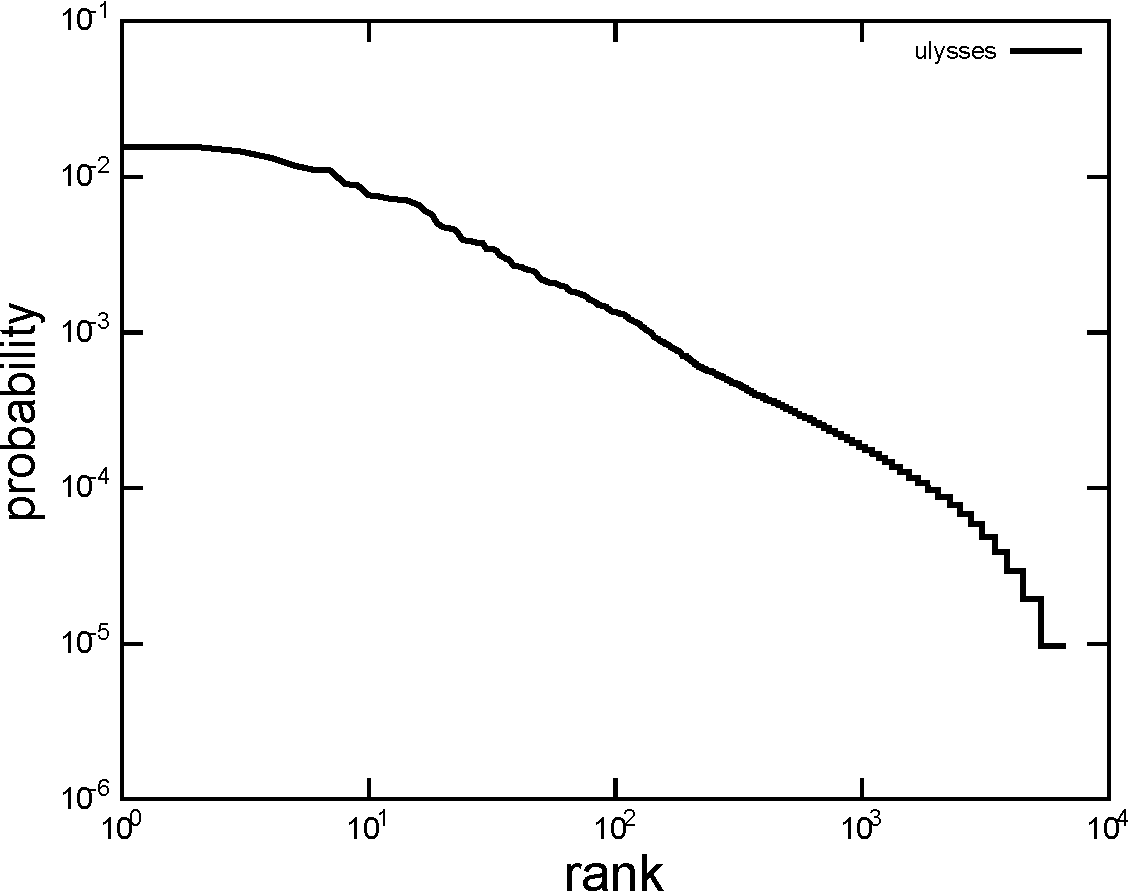
\includegraphics[width=0.7\textwidth]{imagespresentation/ulysses_syllables_probabilities.pdf}
  \caption{Syllable Probability (from \emph{Ulysses)}.}
  \label{fig:ulysses_syllables_probabilities}
  \end{figure} 
}




\frame
{
  \frametitle{Words Length}
\begin{figure}[h!]
\centering
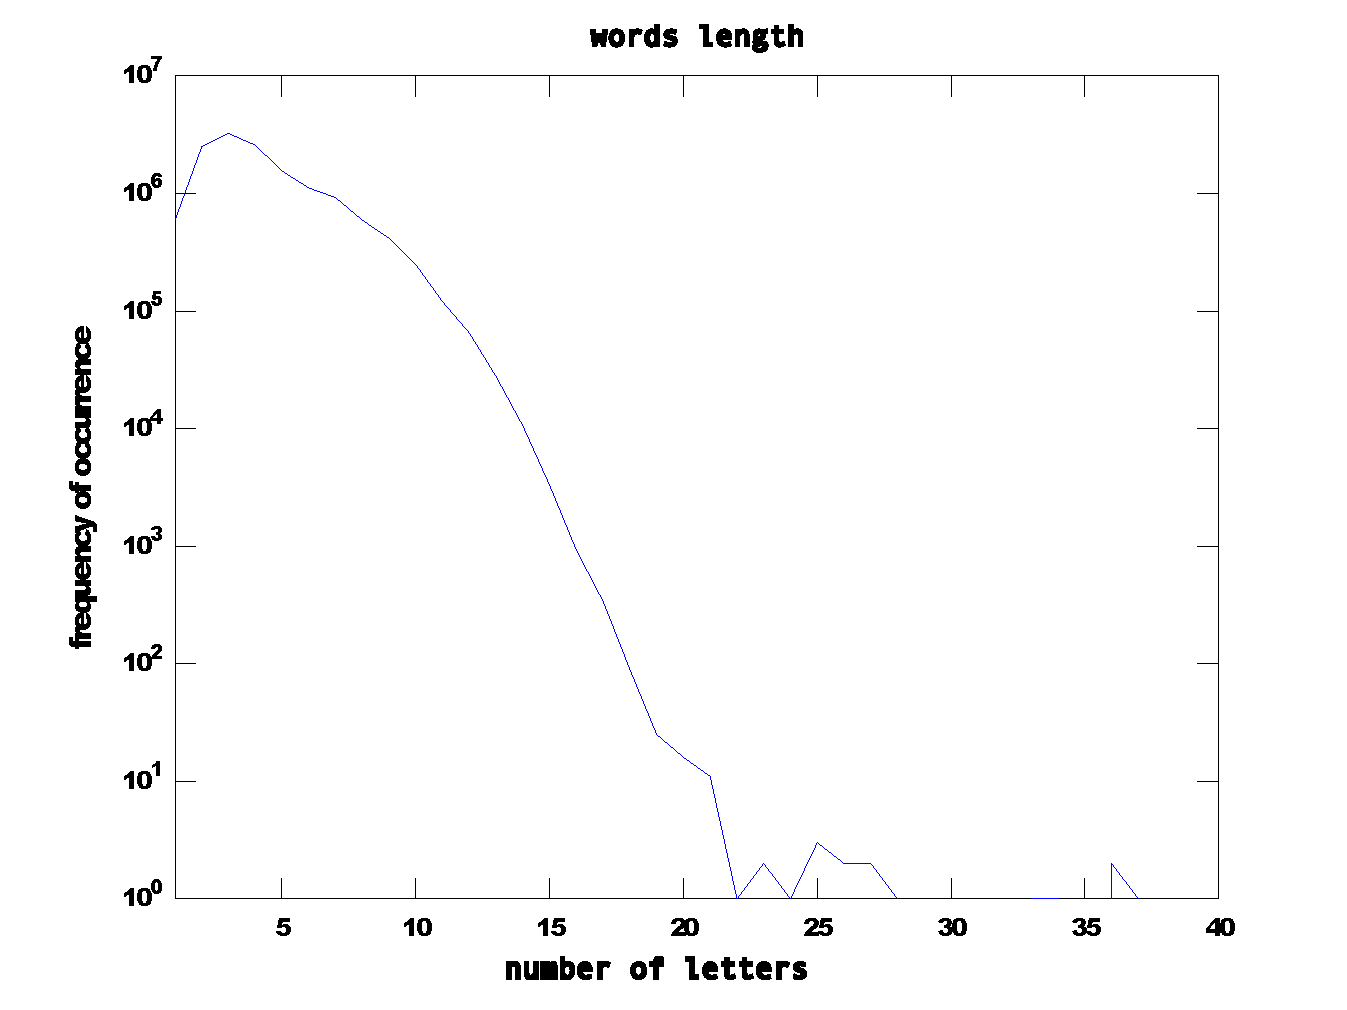
\includegraphics[width=0.7\textwidth]{images/wordslength_en.pdf}
\caption{Frequency of occurrence of words of a given length (letters).}
\label{fig:wordslength_en}
\end{figure}   
}


%\frame
%{
%  \frametitle{Words Length Normalized}
%\vspace{-0.2cm}
%\begin{figure}[h!]
%\centering
%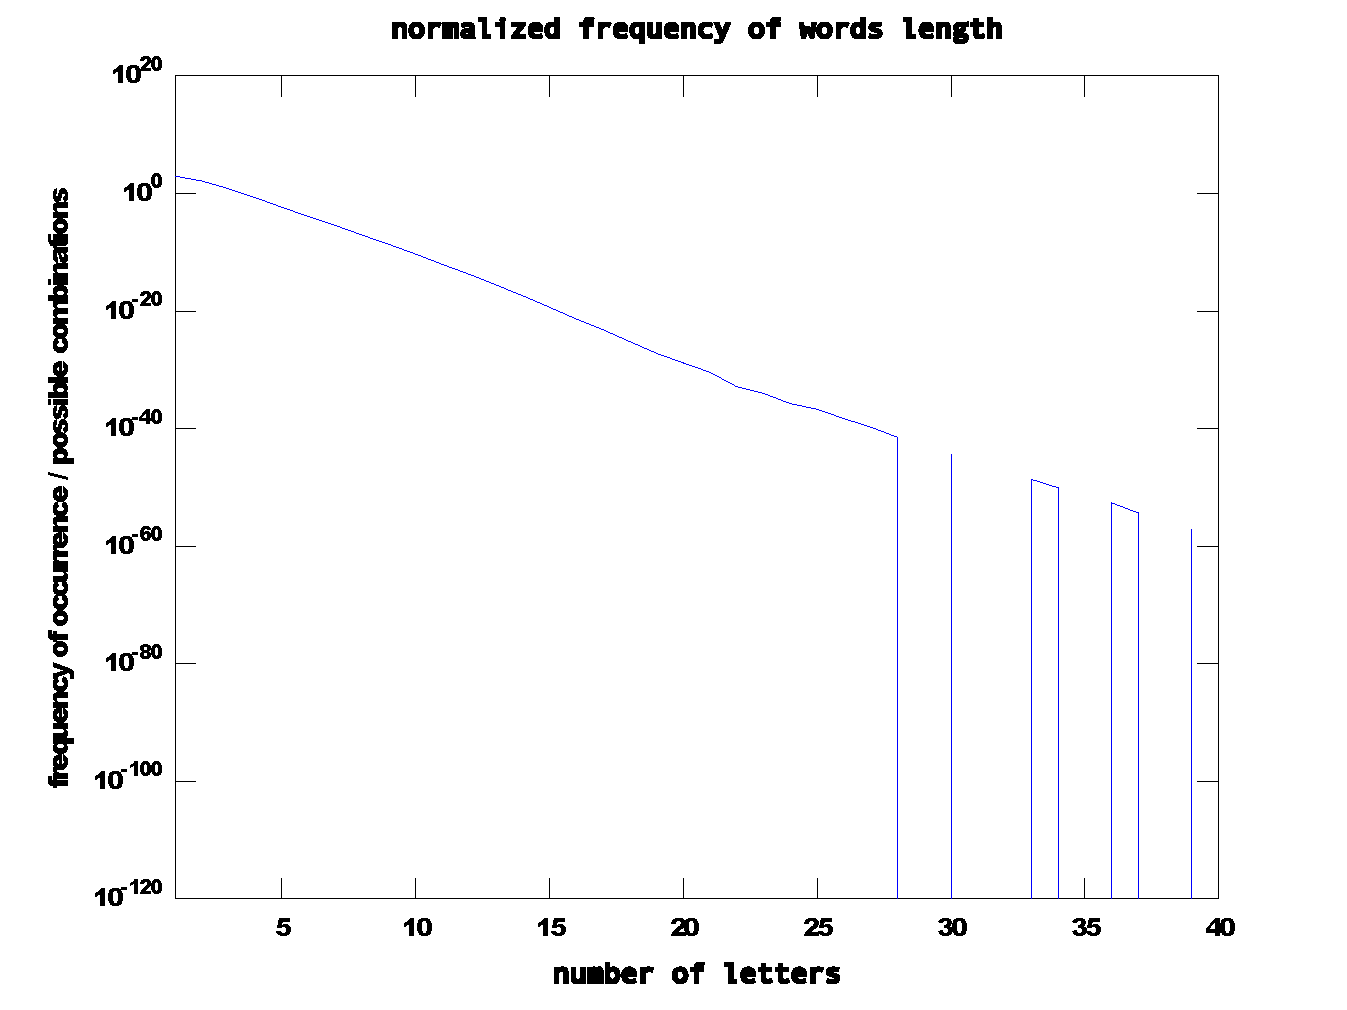
\includegraphics[width=0.7\textwidth]{images/wordslengthfreqnorm_en.pdf}
%\vspace{-0.2cm}
%\caption{Frequency of occurrence of words of a given length (letters) normalized by the total number of  combinations of letters for a given length.}
%\label{fig:wordslengthfreqnorm_en}
%\end{figure}   
%}


\frame
{
  \frametitle{Words Phones Length}
\begin{figure}[h!]
\centering
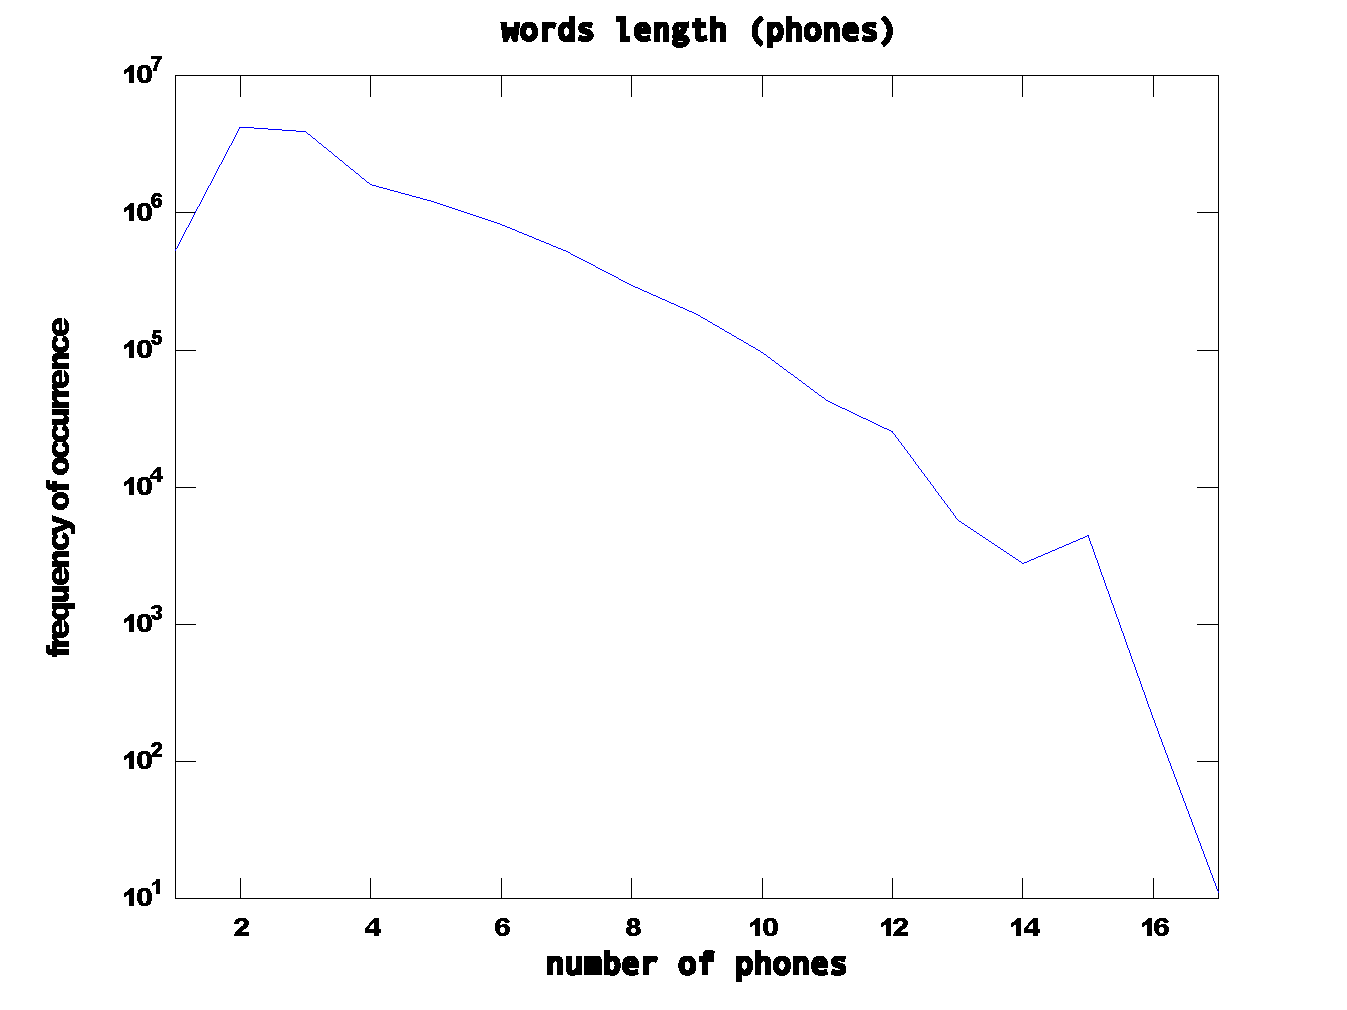
\includegraphics[width=0.7\textwidth]{images/wordsphoneslength_en.pdf}
\caption{Frequency of occurrence of words of a given length (phones).}
\label{fig:wordsphoneslength_en}
\end{figure}   
}
\note{
Fucks (e.g. 1955, 1956) demonstrated both theoretically and empirically that word
length, measured in terms of the number of syllables, follows a displaced Poisson distribution. 

Frequent discrepancies between the data and this model led GROTJAHN (1982) to
consider the parameter of the Poisson distribution as a random variable following a
gamma distribution. This approach yielded a displaced negative binomial distribution
which provided a much better fit than the original Poisson distribution, being merely a
limiting form of the negative binomial.
}
\note{
As long as the empirical data are consistent with the model there is no need for
improvement; this is common practice in all sciences. However, since it can be shown
that a great part of the published data does not fit the above models closely enough, it is
advisable to reconsider the whole problem of modelling the distribution of word length.
}
\note{
In addition to the purely linguistic difficulty of defining the concept of word and of
delimiting wordlike units for example in texts, we encounter six practical and theoretical
problems in modelling the distribution of word length:
\begin{enumerate}[(i)]
\item Up to now word length has been primarily measured in terms of letters, syllables and morphemes, 
      although other possibilities are conceivable. This is the fundamental \emph{problem of the unit of measurement}.
\item There are a number of factors which affect the distribution of word length in
      a specific population. This phenomenon will be referred to as the \emph{population problem}.
\item Different boundary conditions might lead to different models and hence to different 
      laws rather than one general law, which would be the ideal state of affairs.  
      This problem will be referred to as the \emph{modelling problem}.
\end{enumerate}
}
\note{
\begin{enumerate}[(i)]
\setcounter{enumi}{3}
\item The usual criterion for the goodness of fit of a probabilistic model to the data is
      Pearson's chi-square test. This test  -- as well as others based on the divergence
      of the observed frequencies from the expected frequencies -- 
      is however strongly dependent on the sample size. In linguistics, where word length can be measured
      on the basis of texts, dictionaries etc., sample size is often so large that Pearson's
      chi-square test - as well as other power divergence tests --
      necessarily lead to a falsification of the model. This is the \emph{goodness-of-fit problem}.
\item Word length plays a role in the self-regulation of language and is thus partially
      dependent on other linguistic properties. This is the problem of the \emph{interrelation-
      ship of linguistic properties}.
\end{enumerate}
}
\note{
\begin{enumerate}[(i)]
\setcounter{enumi}{5}
\item Knowledge of the interrelationship of word length with other linguistic phenomena 
      as well as of the mechanisms involved in generating the word length patterns
      in various languages, helps us in establishing a valid explanation of the nature of
      word length. This is the \emph{problem of explanation}.
\end{enumerate}
\citep{grotjan2007}
}


%\frame
%{
%  \frametitle{Words Phones Length Normalized}
%  \vspace{-0.2cm}
%\begin{figure}[h!]
%\centering
%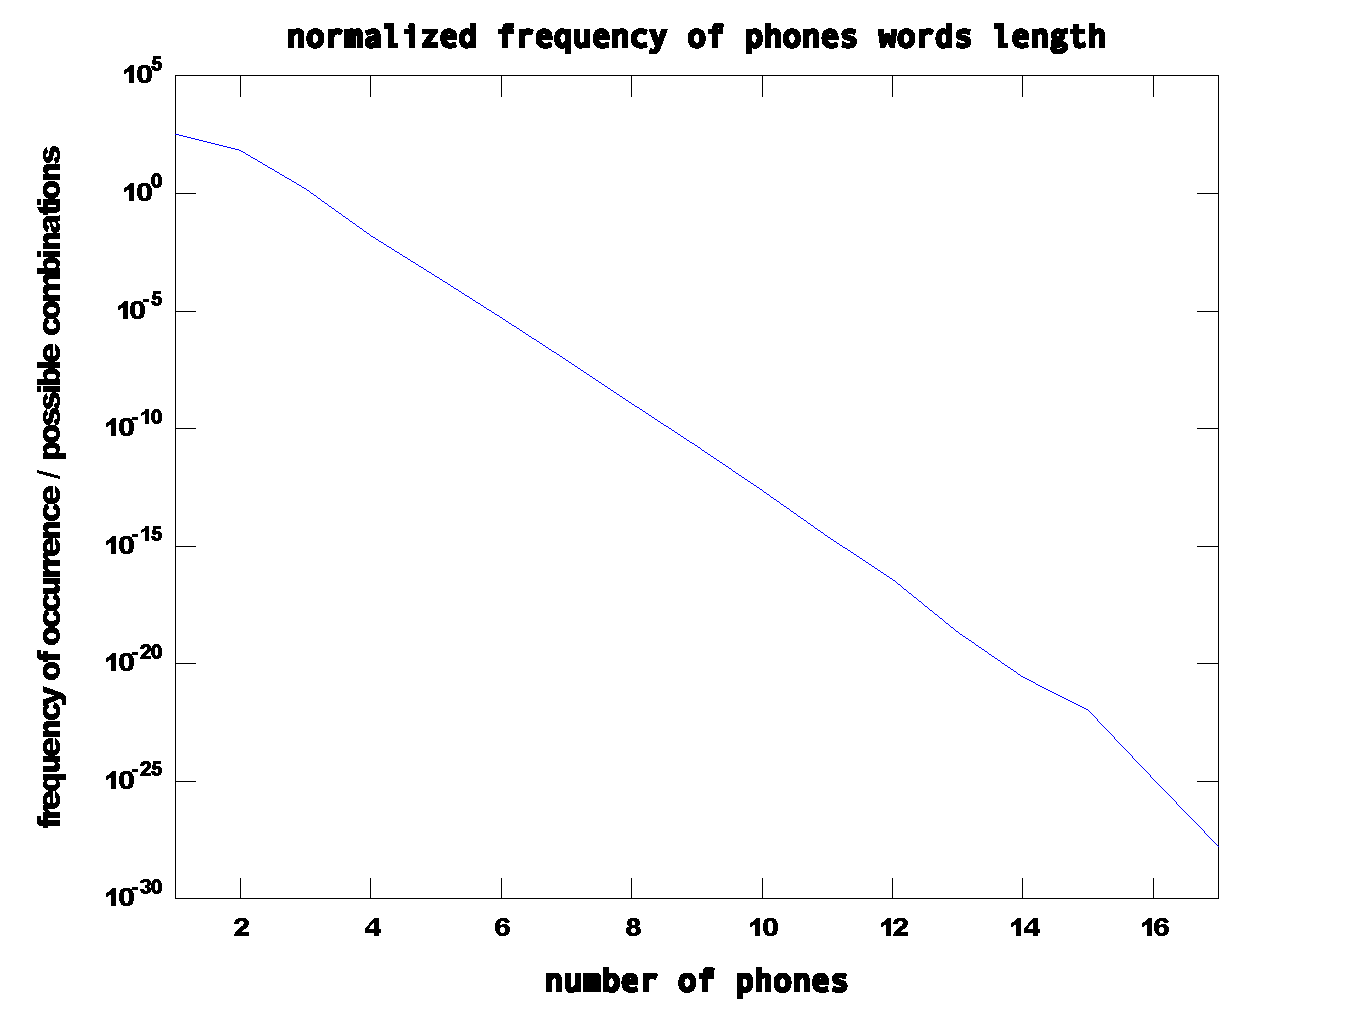
\includegraphics[width=0.7\textwidth]{images/wordsphoneslengthfreqnorm_en.pdf}
%\vspace{-0.2cm}
%\caption{Frequency of occurrence of words of a given length (phones) normalized by the total number of  combinations of phones for a given length.}
%\label{fig:wordsphoneslengthfreqnorm_en}
%\end{figure}   
%}


\frame
{
  \frametitle{Average word length (letters)}
  \vspace{-0.2cm}
\begin{figure}[h!]
\centering
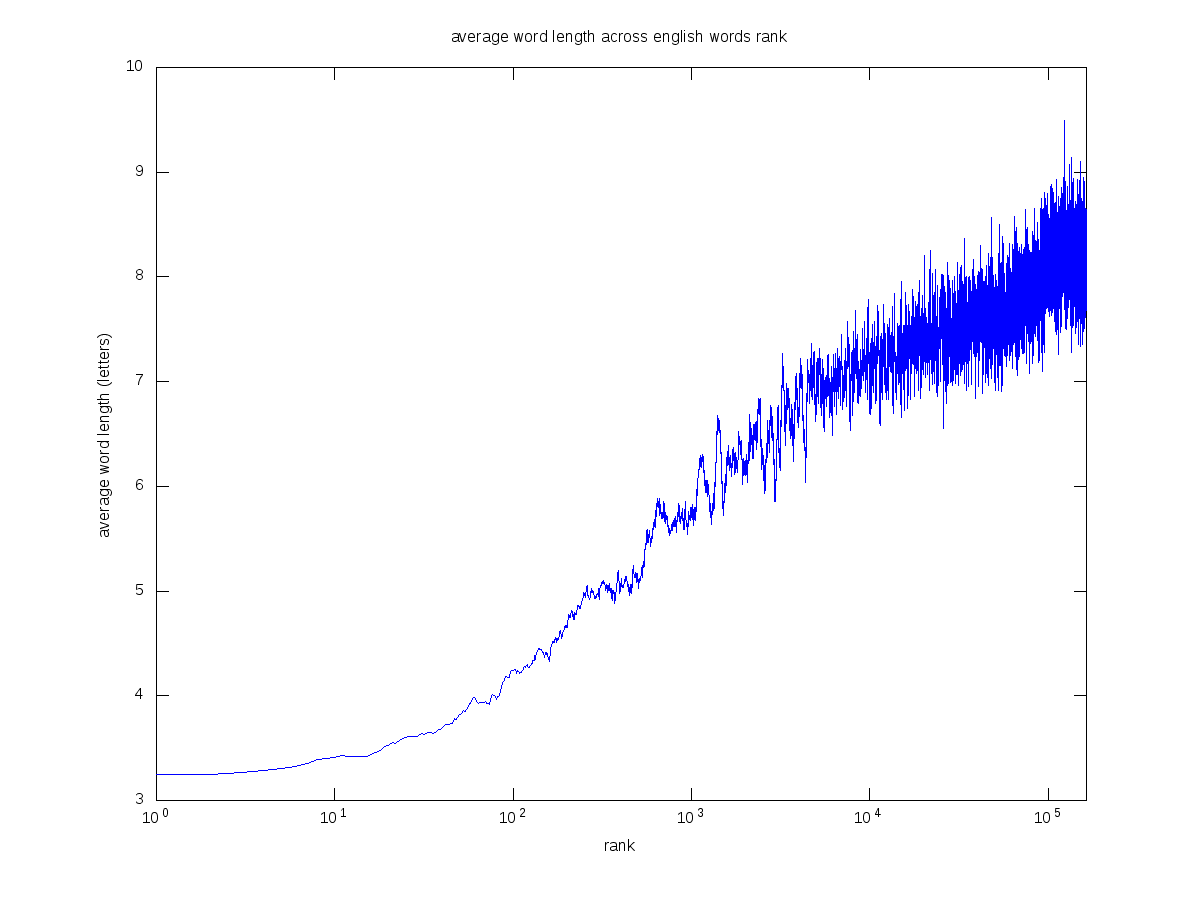
\includegraphics[width=0.75\textwidth]{images/averagewordslength_en.png}
\vspace{-0.2cm}
\caption{Average word length (letters) across word rank.}
\label{fig:averagewordslength_en}
\end{figure}   
}


\frame
{
  \frametitle{Average word length (phones)}
  \vspace{-0.2cm}
\begin{figure}[h!]
\centering
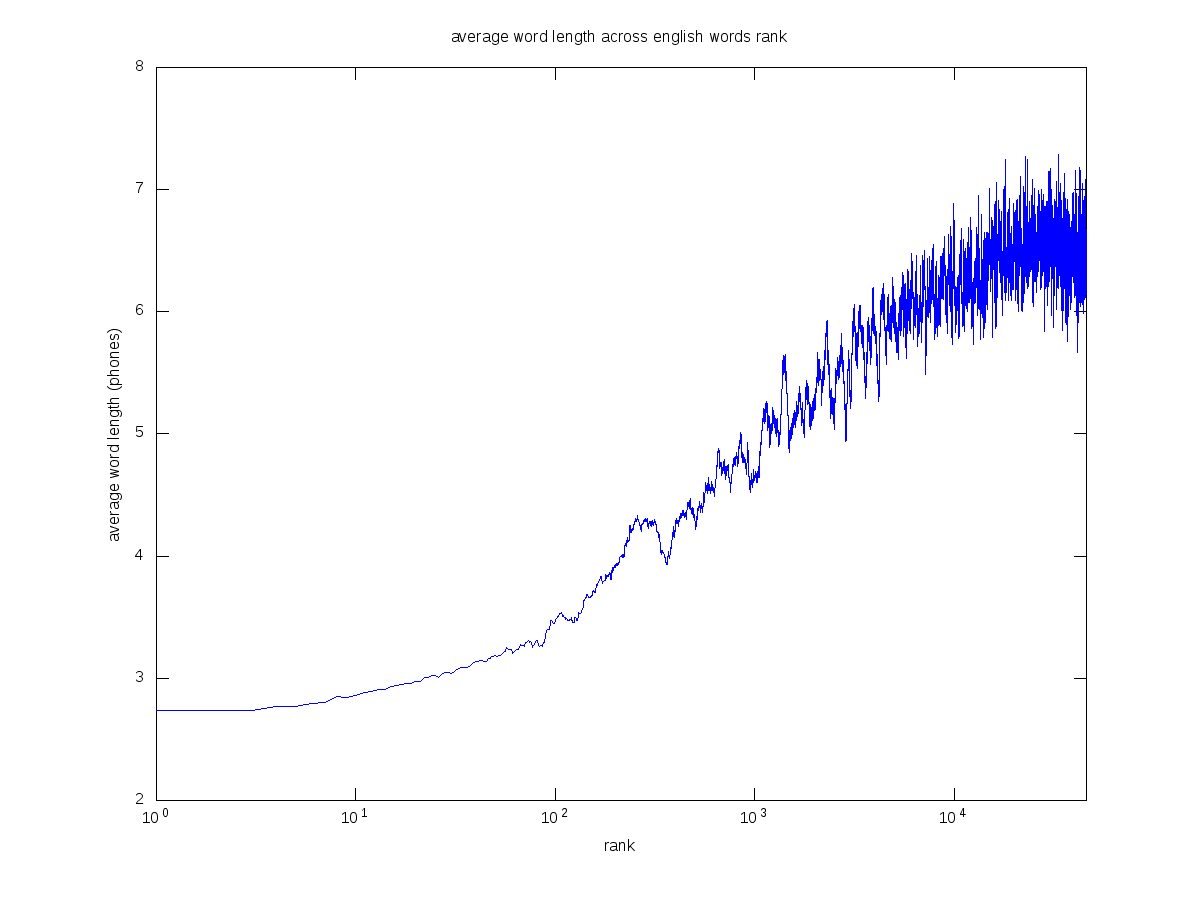
\includegraphics[width=0.75\textwidth]{images/averagewordsphoneslength_en.png}
\vspace{-0.2cm}
\caption{Average word length (phones) across word rank.}
\label{fig:averagewordsphoneslength_en}
\end{figure}   
}


\frame
{
  \frametitle{Frequency of occurrence and frequency index}
  \vspace{-0.2cm}
\begin{figure}[h!]
\centering
\includegraphics[width=0.75\textwidth]{images/wordsFreqIndexVsOccurrence.png}
\vspace{-0.6cm}
\caption{\begin{scriptsize}Each spot represents a word with a given frequency of occurrence and a frequency index. For a better visualization the frequency of occurrence is displayed in a logarithm scale.\end{scriptsize}}
\label{fig:wordsFreqIndexVsOccurrence}
\end{figure}   
}


\frame
{
  \frametitle{Frequency of occurrence vs frequency index (density plot)}
  \vspace{-0.2cm}
\begin{figure}[h!]
\centering
\includegraphics[width=0.75\textwidth]{images/wordsFreqIndexVsOccurrenceDensity.png}
\vspace{-0.6cm}
\caption{\begin{scriptsize}This picture is the density of words in each partition on the frequency of occurrence vs. frequency index space. The largest number is displayed in black and it refers to 578 words. White represents no word found in a spot. \end{scriptsize}}
\label{fig:wordsFreqIndexVsOccurrence}
\end{figure}   
}





\frame
{
  \frametitle{Analysis of Smaller Units}
  Word is considered the smallest free form that can be uttered or written and carries a meaning \citep{bloomfield1926}.
  
  \vspace{1cm}
  Basic units of speech perception:
  \begin{itemize}
  \item phones \citep{pisoni1982}
  \item diphones \citep{klatt1979}
  \item triphones (speech synthesis)
  \item syllables \citep{studdert1976}
  \item demisyllables \citep{fujimura1978} 
  \end{itemize}
} 



\frame
{
  \frametitle{Distinctive Features}

    \begin{figure}[h!]
    \centering
    \includegraphics[width=0.8\textwidth]{imagespresentation/distinctivefeature_en_matrix.png}
    \caption{English Distinctive Features Table.}
    \label{fig:distinctivefeature_en_matrix}
    \end{figure}

}
\note{
The theory proposes the existence of a small finite set of features that may be used to analyze speech sounds, in such way that the description of each speech sound in terms of these features is unique.
The analysis into distinctive features is a unambiguous process to associate speech sounds
into arrays of features that describe these sounds. The features proposed are a conjunction of
perceptual and articulatory factors. The classical statement of distinctive
features was brought by \citet{chomsky1968a}.

The most important contribution to phonology from the distinctive feature theory is
that a set of segments may be analyzed into some features and it is possible to identify
classes of segments in rules, creating the notion of natural class, as a set of sounds that
has certain phonetic features in common and is affected in the same way in the same
environment.
}


\frame
{
  \frametitle{Distinctive Feature Distance}
  
  \begin{block}{definition: distance measure between two segments}
  we define a distance measure of two segments as the number of features not shared between
  them (that dissimilarity definition resembles the natural class definition of \cite{flemming2005})
  \end{block}
}

\frame
{
  \frametitle{Dissimilarity Matrix}
  \vspace{-0.25cm}
  \begin{figure}[h]
  \centering
  \includegraphics[width=0.75\textwidth]{imagespresentation/dissimilarity_en_matrix.png}
  %\caption{}
  \end{figure}
}

\frame
{
  \frametitle{Multidimensional Scaling (MDS)}
  \begin{figure}[h]
  \centering
  \includegraphics[width=\textwidth]{imagespresentation/mdsex.pdf}
  \caption{Simple Multidimensional Scaling Example.}
  \end{figure}
}


\frame
{
  \frametitle{MDS - Vowels}
  \begin{figure}[h]
  \centering
  \includegraphics[width=0.65\textwidth]{imagespresentation/mds_vowels_en.pdf}
  \caption{MDS for English vowels. The first two PCs account for 63\% of variance.}
  \end{figure}
}
\note{
Multidimensional scaling (MDS) is a means of visualizing the level of similarity of individual cases of a dataset.
An MDS algorithm aims to place each object in N-dimensional space such that the between-object distances are preserved as well as possible. Each object is then assigned coordinates in each of the N dimensions. The number of dimensions of an MDS plot N can exceed 2 and are specified a priori. Choosing N=2 optimizes the object locations for a two-dimensional scatterplot.
}


\frame
{
  \frametitle{MDS - Consonants}
  \begin{figure}[h]
  \centering
  \includegraphics[width=0.65\textwidth]{imagespresentation/mds_consonants_en_classes.pdf}
  \caption{MDS for English consonants. The first two PCs account for 46\% of variance.}
  \end{figure}
}


\frame
{
  \frametitle{Intradistances - triphones}
  \vspace{-0.1cm}
  \begin{figure}[h]
  \centering  
  \includegraphics[width=0.8\textwidth]{images/ulysses_triphones_intradistances_mesh.pdf} 
  \caption{Probability of triphones given its intradistances.}
  \end{figure} 
}


\frame
{
  \frametitle{Frequency of occurrence of words in logarithmic scale}
  \vspace{-0.1cm}
  \begin{figure}[h]
  \centering
  \includegraphics[width=0.6\textwidth]{imagespresentation/ulysses_words_intra_phone_distance_freq_occ_avg_std.pdf}
  \caption{Relation in words between frequency of occurrence, average intra-phone distances and standard deviation of these distances.}
  \end{figure}
}





\subsubsection{Zipf law}
\frame
{
  \frametitle{Words Frequency and Zipf Law}
  \vspace{-0.25cm}
  \begin{figure}[h!]
  \centering
  \includegraphics[width=0.8\textwidth]{images/wordfrequency_en.png}
  \vspace{-0.6cm}
  \caption{Log-log plot of words rank versus frequency of occurrence.}
  \label{fig:wordfrequency_en}
  \end{figure} 
}

\frame
{
  \frametitle{Zipf's Law}

 Zipf law states that there is a relationship between the word's frequency of appearance in texts and its rank, the product of them is roughly a constant.
 
 Power law relation: 
 \begin{equation}
 f(k;s,N) = Ck^{-s} = \frac{k^{-s}}{\sum_{n=1}^{N} n^{-s}}
 \end{equation}

 \begin{description}
 \item[f] frequency
 \item[k] rank
 \item[N] number of elements in the set
 \item[s] characterizing exponent
 \end{description}

}
\note{
As already pointed out by \cite{li1992}, ``Zipf's law is not a deep law in natural language as one might first have thought. It is very much related the to particular representation one chooses, i.e., rank as the independent variable.'' \cite{li1992} showed that random texts also exhibit Zipf's law-like curves.
}


\frame
{
  \frametitle{Zipf's Law}
  The normalizing constant $C$ in Zipf's law might also be written as
  \begin{equation}
  C = \frac{1}{H_{N,s}} 
  \end{equation}
  where $H_{N,s}$ is known as the generalized harmonic number
  \begin{equation}
  H_{N,s} = \sum_{n=1}^{N} \frac{1}{n^s} \textmd{ .}
  \end{equation}
  (as $N \rightarrow \infty$, converges for $s>1$)
}



\frame
{
  \frametitle{Zipf's exponent}

  \begin{figure}[h!]
  \centering
  \includegraphics[width=0.7\textwidth]{images/zipfdistribution.png}
  \caption{Probability mass function with $N=10$. (Wikipedia)}
  \end{figure}
}


\frame
{
  \frametitle{The ubiquity of Zipf's law}
  
  This seemingly universal law is present in various phenomena:
  \begin{enumerate}
  \item earthquakes 
  \item avalanches
  \item populations
  \item firms
  \item stocks
  \item game of life
  \item lifespan of genera
  \item etc 
  \end{enumerate}
}



\frame
{
  \frametitle{Gutenberg-Richter law for earthquakes}

  \begin{columns}[c]
  \column{0.4\textwidth}

  Relation between magnitude $m$ of a earthquake and the number $N$ of earthquakes with magnitude greater or equal to $m$:
  \begin{equation}
  \log(N) = -b m + a \textmd{ . }
  \end{equation}

  \begin{equation}
  m = \log_{10} \left( \frac{A}{A_\mathrm{0}(\delta)} \right)
  \end{equation}

  \column{0.6\textwidth}

  \vspace{-0.3cm}
  \begin{figure}[h!]
  \centering
  \includegraphics[width=0.9\textwidth]{images/GutenbergRichter.png}
  \caption{Data from the South of California from 1932 to 1972 \citep{turcotte}.}
  \label{fig:GutenbergRichter}
  \end{figure}

  \end{columns}
}
\note{
The Richter magnitude of an earthquake is determined from the logarithm of the 
amplitude of waves recorded by seismographs (adjustments are included to compensate 
for the variation in the distance between the various seismographs and the 
epicenter of the earthquake). The original formula is:
$M_\mathrm{L} = \log_{10} A - \log_{10} A_\mathrm{0}(\delta) = \log_{10} [A / A_\mathrm{0}(\delta)]$,
where $A$ is the maximum excursion of the Wood-Anderson seismograph, the empirical function 
$A_0$ depends only on the epicentral distance of the station, $\delta$. 
In practice, readings from all observing stations are averaged after adjustment with 
station-specific corrections to obtain the $M_L$ value.
}


\frame
{
  \frametitle{Sandpile}

  \begin{columns}[c]
  \column{0.3\textwidth}
     \begin{figure}[h!]
     \centering
     \includegraphics[width=0.9\textwidth]{images/sandpile.jpg}
     \caption{Sandpile avalanches \citep{bak1999}.}
     \label{fig:sandpile}
     \end{figure}  
  \column{0.7\textwidth}
     \begin{figure}[h!]
     \centering
     \includegraphics[width=0.95\textwidth]{images/sandpileavalancheszipf.png}
     \caption{Frequency of avalanches.}
     \label{fig:sandpileavalancheszipf}
     \end{figure} 
  \end{columns}
}

\frame
{
  \frametitle{Population}

  \begin{columns}[c]
  \column{0.3\textwidth}
     \begin{figure}[h!]
     \centering
     \includegraphics[width=0.9\textwidth]{images/cities.jpg}
     %\caption{}
     \label{fig:cities}
     \end{figure}
  \column{0.7\textwidth}
     \begin{figure}[h!]
     \centering
     \includegraphics[width=0.95\textwidth]{images/glaeserzipf.jpg}
     \caption{Population of American metropolitan areas (Edward L. Glaeser).}
     \label{fig:glaeserzipf}
     \end{figure}
  \end{columns}
}



\frame
{
  \frametitle{Stocks}

  \begin{columns}[c]
  \column{0.4\textwidth}
     \begin{figure}[h!]
     \centering
     \includegraphics[width=\textwidth]{imagespresentation/bovespa.png}
     %\caption{}
     \label{fig:bovespa}
     \end{figure}
  \column{0.6\textwidth}
     \begin{figure}[h!]
     \centering
     \includegraphics[width=0.95\textwidth]{imagespresentation/ibov.pdf}
     \caption{Variations on the Ibov index, using the idea presented by \cite{mandelbrot1963}.}
     \label{fig:glaeserzipf}
     \end{figure}
  \end{columns}
}


\frame
{
  \frametitle{Game of Life}
  
  \begin{columns}[c]
  \column{0.4\textwidth}
  \begin{itemize}
  \item cellular automata (Stanisław Ulam, John von Neumann, 1940)
  \end{itemize}

  \begin{center}
  \animategraphics[autoplay,loop,height=3cm]{1}{/home/leoca/ee/doutorado/2011_1/concurso/ourobranco/projeto/anime/myanime}{0}{29}
  \end{center}

  \column{0.6\textwidth}
     \vspace{-0.3cm}
     \begin{figure}[h!]
     \centering
     \includegraphics[width=0.8\textwidth]{imagespresentation/gameoflife.png}
     \caption{Avalanches (number of births and deaths until a static configuration is reached) in the game of life \citep{paczuski}.}
     \label{fig:gameoflife}
     \end{figure}
  \end{columns}


}
\note{
A cellular automaton (pl. cellular automata) is a discrete model studied in computability theory, mathematics, physics, complexity science, theoretical biology and microstructure modeling. A cellular automaton consists of a regular grid of cells, each in one of a finite number of states, such as on and off. The grid can be in any finite number of dimensions. For each cell, a set of cells called its neighborhood is defined relative to the specified cell. An initial state (time t=0) is selected by assigning a state for each cell. A new generation is created (advancing t by 1), according to some fixed rule (generally, a mathematical function) that determines the new state of each cell in terms of the current state of the cell and the states of the cells in its neighborhood. Typically, the rule for updating the state of cells is the same for each cell and does not change over time, and is applied to the whole grid simultaneously. 
}
\note{
The concept was originally discovered in the 1940s by Stanislaw Ulam and John von Neumann while they were contemporaries at Los Alamos National Laboratory. While studied by some throughout the 1950s and 1960s, it was not until the 1970s and Conway's Game of Life, a two-dimensional cellular automaton, that interest in the subject expanded beyond academia. In the 1980s, Stephen Wolfram engaged in a systematic study of one-dimensional cellular automata, or what he calls elementary cellular automata; his research assistant Matthew Cook showed that one of these rules is Turing-complete. Wolfram published A New Kind of Science in 2002, claiming that cellular automata have applications in many fields of science. These include computer processors and cryptography.
}


\frame
{
  \frametitle{Lifespans of Genera}
  \begin{columns}[c]
  \column{0.5\textwidth}

    \begin{figure}[h!]
    \centering
    \includegraphics[width=\textwidth]{imagespresentation/num_genera_hist.png}
    \caption{Distribution of length of lifespans of genera (in millions of years).}
    \label{fig:num_genera_hist}
    \end{figure}

  \column{0.5\textwidth}

    \begin{figure}[h!]
    \centering
    \includegraphics[width=\textwidth]{imagespresentation/num_genera_loglog.pdf}
    \caption{Loglog plot of the lifespans (data from Sepkoski Fossil Marine Genera Data Warehouse).}
    \label{fig:num_genera_loglog}
    \end{figure}
 
  \end{columns}
}






%\subsubsection{Random Text vs Natural Language}
\frame
{
  \frametitle{Random Texts}
    \begin{figure}[h!]
    \centering
    \includegraphics[width=0.45\textwidth]{imagespresentation/wentianli.png}
    \caption{Word frequency vs \emph{rank} for random generated symbols equally distributed. 
    Symbol set size: $M=2$, $4$, and $6$. Reference Zipf's law for $s=1$ and $2$ are displayed. \citep{li1992,miller1957}}
    \label{fig:wentianli}
    \end{figure}
}


\frame
{
  \frametitle{Random Text vs Ulysses}
    \begin{figure}[h!]
    \centering
    \includegraphics[width=0.6\textwidth]{imagespresentation/ulysses_compared_words_probabilities.pdf}
    \caption{Random text and \textit{Ulysses} compared.}
    \label{fig:ulysses_compared_words_probabilities}
    \end{figure}
}


\frame
{
  \frametitle{Random Texts vs Ulysses: word length}
    \begin{figure}[h!]
    \centering
    \includegraphics[width=0.6\textwidth]{imagespresentation/ulysses_compared_word_length_probabilities.pdf}
    \caption{Word probability for a given length.}
    \label{fig:ulysses_compared_word_length_probabilities}
    \end{figure}
}



\frame
{
  \frametitle{Markov Processes and Zipf's law}
  \cite{kanter1995} shows that a 2-parameter random Markov process constructed with $N$ states and biased
  random transitions gives rise to a stationary distribution where the probabilities of occurrence of the
  states exhibit a rank-ordered frequencies of occurrence of words given by Zipf's law.
}


\frame
{
  \frametitle{Random Text Model - Biemann}
  \cite{biemann2007} proposes a model of Random Text generation that
  takes the properties of neighboring co-occurrence into account
  and introduces the notion of sentences in random text.
 
  \vspace{0.5cm} 
  It is basically composed of: A word generator that produces random words 
  composed of letters and a sentence generator that composes random
  sentences of words.
}
\note{
What distinguishes Biemann's proposal is that it is a hierarchical random text generator.
In a higher level there is the random text generator that creates sentences, and in
a lower level there is the random sentence generator which will create a random
selection of words to built a sentence.
}


\frame
{
  \frametitle{Random Text Model - Biemann}
    \begin{figure}[h!]
    \centering
    \includegraphics[width=0.9\textwidth]{imagespresentation/biemann.pdf}
    \caption{Rank-frequency distribution and lexical spectrum for the word generator in comparison to the Mandelbrot model \citep{biemann2007}.}
    \label{fig:biemann}
    \end{figure}
}
\note{
The creation of this hierarchy in the random text generation makes the resulted text much more 
similar to a true Zippfian distributed process. That is observed in the Zipf's plot and also
on the lexical spectrum plot (inverse Zipf plot).
}




\frame
{
  \frametitle{Zipf Exponent}

  The Zipf's exponent characterizes the source's distribution.

  \begin{itemize}
  \item natural phenomena $1 \leq s \leq 2$ \citep{baek2011}
  \item natural languages $s \approx 1$ \citep{piotrovskii}
  \item children's speech $s \approx 1.66$ \citep{piotrovskii}
  \item military combat text $s \approx 1.42$ \citep{kolguskin1960}
  \item adult and infant dolphins $s \approx 1.1$ and $s \approx 0.87$, respectively \citep{mccowan1999}
  \item authorship attribution \citep{havlin1995}
  \item noncoding DNA sequence $s \approx 0.36$ and coding DNA sequence $s \approx 0.20$ \citep{mantegna1994}
  \end{itemize}
}

\frame
{
  \frametitle{Zipf Fit}
Probability density function for a Zipf distribution:
\begin{equation}
\label{eq:zipf_relation}
f(k | s, N) = \frac{1/k^s}{\sum_{n=1}^{N} n^{-s}} = \frac{1/k^s}{H_{N,s}} ,
\end{equation} 

Maximum likelihood estimation (MLE).

\begin{eqnarray}
L(s|k_1,\cdots,k_M,N) &=& f(k=(k_1, k_2, \cdots, k_M) | s, N) \nonumber \\ 
                      &=& \prod_{m=1}^{M} f(k_m | s, N) \nonumber \\
                      &=& \left( \frac{1}{H_{N,s}} \right)^M \prod_{m=1}^{M} \frac{1}{k_m^s} .
\end{eqnarray}

}


\frame
{
  \frametitle{Zipf Fit}
  The logarithm of the likelihood function:
  \begin{equation}
  \ln L(s|k_1,\cdots,k_M,N) = -M \ln H_{N,s} - s \sum_{m=1}^{M} \ln k_m .
  \end{equation}

  Solution:
  the parameter $s$ such that
  \begin{equation}
  \label{eq:dervloglikelihood}
  \frac{\partial \ln L(s|k,N)}{\partial s} = 0  \textmd{ ,}
  \end{equation}
  if
  \begin{equation}
  \frac{\partial^2 \ln L(s|k,N)}{\partial s^2} < 0 \textmd{ .}
  \end{equation}
}


\frame
{
  \frametitle{Zipf Fit}
  We need to solve
  \begin{equation}
  \frac{\partial \ln L(s|k_1,\cdots,k_M,N)}{\partial s}  = -M \frac{G_{N,s}}{H_{N,s}} - \sum_{m=1}^{M} \ln k_m  = 0 \textmd{ ,}
  \end{equation}

  given that
  \begin{equation}
  \frac{\partial^2}{\partial s^2} \ln L(s|k_1,\cdots,k_M,N) = M \frac{  G_{N,s}^2 - I_{N,s} H_{N,s}  } {H_{N,s}^2} < 0 \textmd{ .}
  \end{equation}

  where
  \begin{equation}
  G_{N,s} = - \sum_{n=1}^{N} n^{-s} \ln n  \textmd{ ,}
  \end{equation}
  \begin{equation}
  I_{N,s} = \sum_{n=1}^{N} n^{-s} \ln^2 n \textmd{ .}
  \end{equation}
}



\frame
{
  \frametitle{Zipf Fit}
  \vspace{-0.3cm}
  \begin{figure}[h]
  \centering
  \includegraphics[width=0.8\textwidth]{imagespresentation/ulysses_fittedcurve_words_probabilities300a.png}
  \caption{Zipf fit to \emph{Ulysses} words ($s_{mle}=1.0738$).}
  \end{figure}
}



\frame
{
  \frametitle{Zipf-Mandelbrot Fit}

The Zipf-Mandelbrot distribution is given by
\begin{equation}
f(k | s, q, N) = \frac{1/(k+q)^s}{\sum_{n=1}^{N} (n+q)^{-s} } = \frac{1/(k+q)^s}{H_{N,s,q}} \textmd{ .} 
\end{equation}

The logarithm of the likelihood is
\begin{equation}
\ln L(s|k_1,\cdots,k_M,N) = -M \ln H_{N,s,q} - s \sum_{m=1}^{M} \ln (k_m+q) \textmd{ .} 
\end{equation}
}


\frame
{
  \frametitle{Zipf-Mandelbrot Fit}
  Now we need to solve:
  \begin{equation}
  \frac{\partial \ln L(s|k_1,\cdots,k_M,N)}{\partial s} = -M \frac{G_{N,s,q}}{H_{N,s,q}} - \sum_{m=1}^{M} \ln (k_m + q) = 0 \textmd{ ,}
  \end{equation}
  \begin{equation}
  \frac{\partial^2 \ln L(s|k_1,\cdots,k_M,N)}{\partial s^2} = M \frac{G_{N,s,q}^2 - I_{N,s,q} H_{N,s,q}}{H_{N,s,q}^2} < 0  \textmd{ .}
  \end{equation}

  \begin{equation}
  \frac{\partial \ln L(s|k_1,\cdots,k_M,N)}{\partial q} = sM \frac{H_{N,s+1,q}}{H_{N,s,q}} - s H_{N,1,q} = 0 \textmd{ ,}
  \end{equation}
  \begin{eqnarray}
  \frac{\partial^2 \ln L(s|k_1,\cdots,k_M,N)}{\partial q^2} &=& s^2 M \frac{H_{N,s+1,q}^2}{H_{N,s,q}^2} - s(s+1)M \frac{H_{N,s+2,q}}{H_{N,s,q}} + \nonumber \\ && + s H_{N,2,q} < 0 \textmd{ .}
  \end{eqnarray}
}


\frame
{
  \frametitle{Zipf-Mandelbrot Fit}
  \vspace{-0.3cm}
  \begin{figure}[h]
  \centering
  \includegraphics[width=0.8\textwidth]{imagespresentation/shakespeare-hamlet.pdf}
  \caption{Zipf-Mandelbrot fit to \emph{Hamlet} words ($s_{mle}=1.087$ $q_{mle}=1.638$).}
  \end{figure}
}




\frame
{
  \frametitle{Lexical Spectrum or Inverse Zipf}
  ``Understanding the origins and evolution of language requires an appropriate
  identification of its universal features. One of the most obvious is the statistical 
  distribution of word abundances. The second
  form is called the lexical spectrum or the inverse Zipf’s distribution''\citep{cancho2002}.

}


\frame
{
  \frametitle{Inverse Zipf}
  
  The number of words for a given frequency of occurrence 
  \begin{equation}
  N(f) = a f^{-\beta}
  \end{equation}
  where 
  \begin{description}
  \item[$N(f)$] number of words with a given frequency $f$
  \item[$f$] frequency of occurrence 
  \item[$a$ and $\beta$] parameters
  \end{description}  


  The exponents are related by
  \begin{equation}
  \beta = \frac{1}{s} + 1 \textmd{ .}
  \end{equation}
}


\frame
{
  \frametitle{Inverse Zipf}
  \begin{figure}[h!]
  \centering
  \includegraphics[width=0.75\textwidth]{images/inverse_zipf_ulysses_words.pdf}
  \caption{Inverse Zipf. Natural and Artificial Texts compared.}
  \label{fig:inverse_zipf_ulysses_words}
  \end{figure} 
}


\frame
{
  \frametitle{Smoothing}
  The maximum likelihood estimator predicts that the probability of a word not seen in the
  corpus is zero.

  \vspace{0.3cm}
  Smoothing is used to overcome this problem.
  \begin{enumerate}
  \item \emph{Add-one} estimator \citep{laplace}
  \item Good-Turing estimator \citep{Good1953}
  \item Simple Good-Turing estimator \citep{galesampson95}
  \end{enumerate}
}


\frame
{
  \frametitle{Good-Turing}
  The Good-Turing method states that
  $N_0 = N_1$ (the total probability of all unseen events is 
  equal to the sum of probabilities of all events that occur only once) and
  the number of observations are adjusted by
  \begin{equation}
  \label{eq:goodturingnormnum}
  f^\ast = (f + 1) \frac{E[N_{f+1}]}{E[N_f]}
  \end{equation}
  
  \begin{description}
  \item[$E\symbol{91} \cdot \symbol{93}$] expectation of a random variable
  \item[$f^\ast$] adjusted number of observations
  \item[$f$] observed frequency of occurrence 
  \item[$N_f$] number of types observed $f$ times
  \end{description}
}


\frame
{
  \frametitle{Simple Good-Turing}
  \cite{galesampson95} proposes a simple way to do a Good-Turing estimation by choosing $E[\cdot]$ so that
  \begin{equation}
  \label{eq:goodturingestimator}
  E[N_{f+1}] = E[N_f] \left( \frac{f}{f+1} \right) \left( 1 - \frac{E[N_1]}{N} \right)
  \end{equation}
  leading to
  \begin{equation}
  p^\ast_f = p_f \left( 1 - \frac{E[N_1]}{N} \right) \textmd{ .}
  \end{equation} 
}

\frame
{
  \frametitle{Simple Good-Turing}

  \begin{figure}[h!]
  \centering
  \includegraphics[width=0.70\textwidth]{images/inverse_zipf_sgt.pdf}
  \caption{Simple Good-Turing.}
  \label{fig:inverse_zipf_sgt}
  \end{figure}
}


\frame
{
  \frametitle{How Zipf's law emerges}
  According to \cite{ramon2003,ferrer05}, Zipf's law is a manifestation
  of a complex system operating between order and disorder.

  \vspace{0.5cm}
  A communication system should minimize $\Omega$ 
  \begin{equation}
  \Omega(\lambda) = - \lambda I(S,R) + (1-\lambda) H(S) \textmd{ ,}
  \end{equation}
  where
  \begin{description}
  \item[S] set of signs (words)
  \item[R] set of estimula 
  \item[I(S,R)] transmitted information 
  \item[H(S)] cost (entropy of words) 
  \end{description}
}

\frame
{
  \frametitle{How Zipf's law emerges}
  \vspace{-0.8cm}
  \begin{figure}
      \begin{subfigure}[b]{0.5\textwidth}
          \centering
          \vtop{
          \includegraphics[width=0.9\textwidth]{images/cancho_figA.pdf}
          \vspace{-0.2cm}
          \caption{\scriptsize $I(S, R)$, the information transfer between words and meanings, versus $\lambda$, the parameter regulating the balance between maximizing $I(S, R)$ and minimizing the entropy of words.}
          \label{fig:cancho_figA}
          }
      \end{subfigure}%
       ~
      \vspace{0pt}
      \begin{subfigure}[b]{0.5\textwidth}
          \centering
          \vtop{
          \includegraphics[width=0.9\textwidth]{images/cancho_figB.pdf}
          \vspace{-0.2cm}
          \caption{\scriptsize $P(i)$, the probability of the $i$-th most likely word in the system for $\lambda  = 0.49$ (circles), $\lambda = 0.498$ (squares) and $\lambda = 0.5$ (diamonds). The dashed line contains the theoretical curve for $\lambda = 0.498$.}
          \label{fig:cancho_figB}
          }
      \end{subfigure}
      \vspace{-0.6cm}
      \caption{\scriptsize Some computational results on the model where meaning probabilities are governed by the internal structure of the communication system. The size of the system is $n = m = 400$ (i.e. 400 words and meanings). Figure reproduced from \cite{cancho2005}.}
        \label{fig:cancho}
\end{figure}
}



\frame
{
  \frametitle{Entropy of a Zipfian Source}
  Entropy of a Zipfian distributed source:
  \begin{eqnarray}
  \label{eq:ent_zipfian_source}
  \overline{H} &=& -\frac{1}{\ln 2} \sum_{k=1}^N Ck^{-s} \ln (Ck^{-s}) \nonumber \\
               &=& \frac{sC}{\ln 2} \sum_{k=1}^N \frac{\ln k}{k^s} - \frac{\ln C}{\ln 2} \textmd{ .}
  \end{eqnarray} 

  We propose lower and upper bounds to estimate the entropy
  \begin{equation}
  B_l \leq \sum_{k=1}^{N} k^{-s} \ln k \leq B_u \textmd{.}
  \end{equation}

}


\frame
{
  \frametitle{Entropy of a Zipfian Source}
  \begin{figure}[h]
  \centering
  \includegraphics[width=0.75\textwidth]{images/logk_ks.pdf}
  \caption{Function $f(x)=\ln x / x^s$ for different values of $s$.}
  \label{fig:logk_ks}
  \end{figure}
}

\frame
{
  \frametitle{Entropy of a Zipfian Source}
  \begin{figure}[h]
  \centering
  \includegraphics[width=0.75\textwidth]{images/logk_k_integral.pdf}
  \caption{Left Riemann sum approximation of the integral.}
  \label{fig:logk_k_integral}
  \end{figure}
}


\frame
{
  \frametitle{Entropy of a Zipfian Source}
  The bounds are given by
  \begin{eqnarray}
  \label{eq:riemmansumeboundsfinal}
  B_l &=& \int_{3}^{N} \frac{\ln x}{x^s} dx + \frac{\ln 2}{2^s} + \frac{\ln N}{N^s} \nonumber \\ 
      &\leq& \sum_{n=1}^{N} \frac{\ln n}{n^s} \nonumber \\
      &\leq& \int_{3}^{N-1} \frac{\ln x}{x^s} dx + \frac{\ln 3}{3^s} + \frac{\ln 2}{2^s} + \frac{\ln N}{N^s} = B_u \textmd{ ,}
  \end{eqnarray}

  and the estimated Entropy is bounded by
  \begin{equation}
  \frac{sC}{\ln 2} B_l - \frac{\ln C}{\ln 2} =  H_l \leq  \overline{H} \leq H_u = \frac{sC}{\ln 2} B_u - \frac{\ln C}{\ln 2} \textmd{ .}
  \end{equation}
}


\frame
{
  \frametitle{Entropy of a Zipfian Source}
  \vspace{-0.5cm}
  \begin{figure}[h]
  \centering
  \includegraphics[width=0.8\textwidth]{imagespresentation/entropy_N_s_limits_fulldh_pb2.pdf}
  \vspace{-0.2cm}
  \caption{\scriptsize Entropy $H$ (in bits) as a function of the Zipf exponent $s$ and the number of types $N$. The upper plot presents the average Entropy estimated and the lower plot presents the difference between the upper and lower bounds of the entropy estimated.}
  \label{fig:entropy_N_s}
  \end{figure}
}


\frame
{
  \frametitle{Entropy of a Zipfian Source}
  \vspace{-0.5cm}
  \begin{figure}[h]
  \centering
  \includegraphics[width=0.8\textwidth]{images/zipfmandelbrot_entropy_sq_surface.pdf}
  \caption{Effect of the parameters $s$ and $q$ on the entropy $H$ (in bits) for a Zipf-Mandelbrot distribution.}
  \label{fig:zipfmandelbrot_entropy_sq_surface}
  \end{figure}
}


\frame
{
  \frametitle{Entropy of a Zipfian Source}
\begin{table}[h!]
\scriptsize
\centering
\caption{\small Entropy of real texts (bits), with and without SGT smoothing, compared with the estimated entropy (bits) using the parameter $N$ (number of types) found in the text, parameter $s$ (Zipf exponent) found by a Maximum Likelihood Estimation (MLE) and the flattening parameter $q$, also found by MLE.}
\label{tab:entropytexts2}
\resizebox{\textwidth}{!}{%
\begin{tabular}{| l | c | c | c | c | c | c | c | c | }
  \hline
  \multirow{3}{*}{source} & \multirow{3}{*}{$N$} & \multicolumn{3}{| c |}{estimated parameters} & \multicolumn{2}{| c |}{entropy} & \multicolumn{2}{| c |}{estimated entropy}  \\ \cline{3-5} \cline{6-7} \cline{8-9}
  & & Zipf & \multicolumn{2}{| c |}{Zipf-Mandelbrot} & \multirow{2}{*}{normal} & \multirow{2}{*}{sgt} & \multirow{2}{*}{Zipf} & \multirow{2}{*}{\begin{tabular}{@{}c@{}}Zipf- \\ Mandelbrot\end{tabular}} \\ \cline{3-5}
  & & s & s & q &  &  &  &  \\
  \hline
  Alice         & 3016  & 0.992 & 1.172 & 3.27 & 8.49  & 8.79  & 8.55  & 8.73 \\
  Hamlet        & 5447  & 0.991 & 1.087 & 1.64 & 9.04  & 9.08  & 9.09  & 9.13 \\
  Macbeth       & 4017  & 0.969 & 1.009 & 0.56 & 9.00  & 9.00  & 9.02  & 9.04 \\
  Shakespeare   & 29847 & 1.060 & 1.172 & 2.33 & 9.52  & 9.57  & 9.60  & 9.69 \\
  Ulysses       & 34391 & 1.025 & 1.085 & 1.18 & 10.19 & 10.25 & 10.22 & 10.25 \\
  \hline
\end{tabular}
}
\end{table} 

}


\frame
{
  \frametitle{Heaps' law (Herdan's law)}

  There is a relation between 
  \begin{description}
  \item[$T$] text size
  \item[$V_T$] vocabulary length
  \end{description}

  given by
  \begin{equation}
  \label{eq:heaps}
  V_T \propto T^\alpha \textmd{ , \ \ } \alpha < 1 \textmd{ .}
  \end{equation}

  \cite{vanLeijenhorst} shows that a Zipfian distributed source 
  presents this relation between text size and vocabulary length.
}


\frame
{
  \frametitle{Heaps' law (Herdan's law)}  
  The expected number of types is monotonically increasing with the sample size. 
  It converges to the length of the underlying lexicon.

  \begin{figure}[h]
  \centering
  \includegraphics[width=0.6\textwidth]{images/heapslaw_rdist.pdf}
  \caption{The recurrence equation is used to estimate the expected number of types for a sample with a certain number of tokens.}
  \label{fig:heapslaw_rdist}
  \end{figure} 
}


\frame
{
  \frametitle{Heaps' law (Herdan's law)}
  \vspace{-0.3cm}
  \begin{figure}[h]
  \centering
  \includegraphics[width=0.8\textwidth]{images/heapslawtexts.png}
  \caption{The relation between the number of tokens and types in 35 books from Gutenberg Database is presented in gray.} 
  \label{fig:heapslawtexts}
  \end{figure}
}


\frame
{
  \frametitle{Menzerath's law}
  The longer the whole, the smaller the parts.

  \cite{menzerath1928} observed the decreasing relation between syllable's length and length of a word (number of syllables).

  \vspace{0.3cm}
  The change relative rate on the length of the constituent is inversely proportional to the length of the construct.
  \begin{equation}
  \frac{y'}{y} = \frac{b}{x} \textmd{.}
  \end{equation}
  \begin{description}
  \item[y] constituent length 
  \item[x] construct length
  \end{description}
  Solution: $y = a x^b$. 

}


\frame
{
  \frametitle{Menzerath's law}
  \begin{figure}
        \begin{subfigure}[b]{0.5\textwidth}
                \centering
                \vtop{
                \includegraphics[width=\textwidth]{images/boxplot_ulysses_words_avg_syllable_duration_ms.pdf}
                \caption{Average syllable duration as words get longer (number of syllables).}
                \label{fig:boxplot_ulysses_words_avg_syllable_duration}
                }
        \end{subfigure}%
        ~ 
        \begin{subfigure}[b]{0.5\textwidth}
                \centering
                \vtop{
                \includegraphics[width=\textwidth]{images/boxplot_ulysses_words_avg_phone_duration_ms.pdf}
                \caption{Average phone duration as words get longer (number of phones).}
                \label{fig:boxplot_ulysses_words_avg_phone_duration}
                }
        \end{subfigure} 
        \label{fig:boxplot_ulysses_words_avg_duration}
  \end{figure}
}


\frame
{
  \frametitle{Menzerath's law}
  \vspace{-0.3cm}
  \begin{figure}[h]
  \centering
  \includegraphics[width=0.8\textwidth]{images/ulysses_words_sentence_word_length_syllables_z100.png}
  \caption{Relation between sentence length (number of words) and average words length (number of syllables) in a sentence.}
  \label{fig:ulysses_words_sentence_word_length}
  \end{figure}
}



\frame[allowframebreaks]
{
  \frametitle{Conclusions}
  \begin{itemize}
  \item usage-based driven language \citep{bybee2001,bybee2003,bybee2007frequency,ellis2002}
  \item humans track co-occurrence patterns and statistical regularities \citep{saffran1996b,Saffran1999,Saffran2003}
  \item regularities among several languages
    \begin{itemize}
    \item some speech segments are very common (example: \textipa{[m]} appear in 94.2\% of the languages)
    \item 427 out of 919 speech sounds appear just once among all 425 languages
    \item 90\% of the languages use at most 6 times more consonants than vowels
    \item a few phones have many co-occurring segments in their languages and are also found in many different languages (wildcards)
    \end{itemize}
  \item ubiquity of scaling laws in nature 
  \item a compared study of `intermittent silence', Markov model and natural text 
  \item compare different sources using the Zipf-Maldelbrot model
  \item mle method to fit the best model
  \item entropy estimation estimation of a Zipf-Maldelbrot source
  \item Menzerath's law and Heap's law
  \item distance measure between phones using Feature Theory
  \end{itemize}
}
\note{
It is important to note that the 425 languages in the UPSID are chosen
so that they represent well all family branches in the language tree. 

We adopt here a usage-based theory of language in which its cognitive 
organization is based directly on one's experience with it, rather
than being an abstract set of rules or structures that are only indirectly 
related to experience with language. We see grammar as a network built up from 
the categorized instances of language use.

Since the grammar is based on usage, it contains many details of co-occurrence as 
well as a record of the probabilities of occurrence and co-occurrence. The evidence for 
the impact of usage on cognitive organization includes the fact that language users are 
aware of specific instances of constructions that are conventionalized and the multiple 
ways in which frequency of use has an impact on structure.
}
\note{
The latter include speed of 
access related to token frequency, priming, morphological and phonetic properties of 
high and low frequency words, as well as the importance of usage to the process of
grammaticalization.

(In linguistics, grammaticalization is a process by which words representing objects and 
actions (i.e. nouns and verbs) transform through sound change and language migration to 
become grammatical markers (affixes, prepositions, etc.).)
}
\note{
A number of recent experimental studies \citep{saffran1996,Saffran1999,Saffran2003} show that both 
infants and adults track co-occurrence patterns and statistical regularities in artificial 
grammars. Such studies indicate that subjects learn patterns even when the grammar 
corresponds to no meaning or communicative intentions. It is thus not surprising that in 
actual communicative settings, the co-occurrence of words has an impact on cognitive 
representation. There is indeed evidence from multiple sources that such cognitive 
changes occur, and contribute to the shape of grammar.

The cognitive representations underlying language use are built up by the categorization of 
utterances into exemplars and exemplar clusters based on their linguistic form as well as 
their meaning and the context in which they have been experienced \citep{pierrehumbert2001}.

The fact that proposed `universals of grammar'
appear to be highly general can be seen as a by-product of this process: 
grammars are emergent phenomena dependent on idiosyncratic localized interactions.
}
\note{
The ubiquity of scaling laws in nature suggests that complex systems organize themselves, 
they are not just a collection of random independent realizations, but exhibit
similar patterns and relations that are observed in different scales.
Complex systems are more than mere collections of independent random variables, they
have interdependent effects and behaviours.
}
\note{
Only the Markov model was able to result in similar patterns to those observed in natural texts.
Frequency of 1-gram, 2-grams, 3-grams, `word' length, occurrence of hapax legomenon,
Zipf and inverse Zipf (lexical spectrum) relations.
}
\note{
The exponent parameter in the Zipf distribution is important to determine the statistical 
properties of that distribution. We observe that different type of sources present 
different exponent values and we argue that this exponent is related to the balance between
order and disorder in a Complex System, the amount of information produced by the source
and the underlying lexicon size (and the possibility of being virtually infinite).
In order to compare data that follow a power law
relation, we need to find the best fit to the data. We have presented the usage of the
maximum likelihood approach to determine the exponent parameters that gives the best
fit. We have derived the equations which lead to a root finding problem, for which the
solution is the maximum likelihood estimated parameter. The same procedure is used to
find the exponent and flattening parameters of a Zipf-Mandelbrot model. This procedure
was tested using real text data and the results show a good performance.
}
\note{
Menzerath's law states a relation on the usage of tiles to create a whole. According to
this law, the length of the whole is inversely proportional to the length of the parts. 

\vspace{0.3cm}
Heap's law: sublinear relation between the text length and the vocabulary size.
Zipf's law implies Heap's law, but any distribution would lead to a convergent sublinear lexical growth
in relation to the text length.
}
\note{
The Feature Theory might be providential since it give us a direct and formal way to
quantify a phone characteristics making it possible to create a distance measure between
two phones. We propose to measure the distance between two phones by the number
of distinctive features not shared by them. We believe this measure might be a meaningful choice.
It could be used alongside frequency of occurrence to draw better explanations to phonological process
and cognitive representation.
}



%\frame
%{
%  \frametitle{MDS - 2D}
%  \vspace{-0.5cm}
%\begin{figure}[h!]
%\centering
%\includegraphics[width=0.95\textwidth]{images/mds_en.pdf}
%%\caption{Dissimilarity matrix for the speech sounds in English.}
%\label{fig:mds_en}
%\end{figure}   
%}


%\frame
%{
%  \frametitle{MDS - 3D}
%  \vspace{-0.5cm}
%\begin{figure}[h!]
%%\centering
%\includegraphics[width=0.95\textwidth]{images/mds_en_3D.pdf}
%%\caption{Dissimilarity matrix for the speech sounds in English.}
%\label{fig:mds_en}
%\end{figure}   
%}
 



%\frame
%{
%  \frametitle{Frequency of occurrence of distinctive features}
%\begin{figure}[h!]
%\centering
%\includegraphics[width=0.85\textwidth]{images/distinctiveFeaturesFreq.pdf}
%%\caption{Frequency of occurrence of distinctive features in English.}
%\label{fig:distinctiveFeaturesFreq}
%\end{figure}  
%}


%\frame
%{
%  \frametitle{Frequency of distinctive features - loglog plot}
%\vspace{-0.3cm}
%\begin{figure}[h!]
%\centering
%\includegraphics[width=0.75\textwidth]{images/distinctiveFeaturesZipf.pdf}
%\vspace{-0.3cm}
%\caption{Distinctive features in English ranked by their frequencies of occurrence.}
%\label{fig:distinctiveFeaturesZipf}
%\end{figure}
%}


%\frame
%{
%  \frametitle{Frequency of cooccurrence of distinctive features}
%  \vspace{-0.3cm}
%\begin{figure}[h!]
%\centering
%\includegraphics[width=0.75\textwidth]{images/distinctiveFeaturesCooccurrenceFreq.png}
%\vspace{-0.5cm}
%\caption{Frequency of cooccurrence of distinctive features in diphones.}
%\label{fig:distinctiveFeaturesCooccurrenceFreq}
%\end{figure}
%}



%\frame
%{
%  \frametitle{Distinctive features frequency - features MDS}
%  \vspace{-0.4cm}
%\begin{figure}[h!]
%\centering
%\includegraphics[width=0.8\textwidth]{images/distinctiveFeaturesMDS.pdf}
%\vspace{-0.5cm}
%\caption{MDS result for the distinctive features in English.}
%\label{fig:distinctiveFeaturesMDS}
%\end{figure}
%}  
  
  

%\section{Further Work}
%
%\frame
%{
%  \frametitle{Further Work}
%  \begin{itemize}
%  \item extend this approach to other languages: intralanguage and interlanguage analysis
%  \item computer simulation: agents, self-organization and statistics \citep{steels97,deboer01}
%  \end{itemize}
%}
%
%
%\subsection{Browsing}
%
%%\frame
%{
%  \frametitle{Browsing Interface : Phones sorted by frequency}
%\begin{figure}[h!]
%\centering
%\includegraphics[width=0.5\textwidth]{images/menu01.png}
%%\caption{Browsing interface to the English phones.}
%\label{fig:menu01}
%\end{figure} 
%
%\href{http://www.cefala.org/~leoca/research/phonesmenu/phonemenu.html}{online example}
%}
%
%\frame
%{
%  \frametitle{Browsing Interface : Diphones sorted by frequency}
%\begin{figure}[h!]
%\centering
%%\includegraphics[width=0.5\textwidth]{images/menu02.png}
%%\caption{Browsing interface to the English phones.}
%\label{fig:menu02}
%\end{figure} 
%}
%
%
%\frame
%{
%  \frametitle{Browsing Interface : Triphones sorted by frequency}
%\begin{figure}[h!]
%\centering
%\includegraphics[width=0.5\textwidth]{images/menu03.png}
%%\caption{Browsing interface to the English phones.}
%\label{fig:menu03}
%\end{figure} 
%}
%
%
%\frame
%{
%  \frametitle{Browsing Interface : Semantic Web}
%\begin{figure}[h!]
%\centering
%\includegraphics[width=0.6\textwidth]{images/semanticweb01.png}
%%\caption{Semantic Web Example for Portuguese.}
%\label{fig:semanticweb01}
%\end{figure} 
%
%\href{http://www.cefala.org/~leoca/research/semanticweb/semanticweb_casa.html}{online example (casa)}
%}
%
%
%\frame
%{
%  \frametitle{Browsing Interface : Semantic Web}
%\begin{figure}[h!]
%\centering
%\includegraphics[width=0.65\textwidth]{images/semanticweb02.png}
%%%\caption{Semantic Web Example for Portuguese.}
%\label{fig:semanticweb02}
%\end{figure} 
%}
%
%
%\subsection{Rosetta Project}
%
%\frame
%{
%  \frametitle{Rosetta Project -  Long Now Foundation}
%  \begin{columns}[c]
%  \column{0.35\textwidth}
%
%  \begin{figure}[h!]
%  \centering
%  \includegraphics[width=0.95\textwidth]{images/rosetta.png}
%  \caption{Rosetta Disk}
%  \label{fig:rosetta}
%  \end{figure} 
%  
%  \column{0.65\textwidth}
%  
%  \begin{figure}[h!]
%  \centering
%  \includegraphics[width=\textwidth]{images/Long_Tail_of_Languages.jpg}
%  \caption{Fifty to ninety percent of the world's languages (in red) are predicted to disappear in the next century.}
%  \label{fig:Long_Tail_of_Languages}
%  \end{figure} 
%  
%  \end{columns}
%}
%\note
%{
%  Rosetta Project is a global collaboration project by Long Now Foundation, with the aid of language specialists and native speakers, to build a contemporary Rosetta Stone. The Rosetta Project collection has grown to over 100,000 pages of documents, as well as language recordings, for over 2,500 languages. 
%}
%\note{
%The materials in the collection were gathered from archives around the world, and include different kinds of language data: descriptions of the community of speakers, maps of their location, and information on writing systems and literacy. There is also grammatical information, including descriptions of sounds used in the language, how words and larger linguistic structures like sentences are formed, a basic vocabulary list (known as a ``Swadesh List''), and texts. Many of the texts are transcribed oral narratives. Others are translations such as the beginning chapters of the Book of Genesis or the UN Declaration of Human Rights. The first three chapters of Genesis were collected in as many languages as possible, to provide a parallel text for language decipherment in the distant future (inspired by the original Rosetta Stone).
%}
%
%
%
%\subsection{Breakthrough}
%\frame
%{
%  \frametitle{Donald Davidson}
%\begin{quote}
%``I conclude that there is no such thing as a language, not if a language is anything like what many philosophers and linguists have supposed. There is therefore no such thing to be learned, mastered, or born with. We must give up the idea of a clearly defined shared structure which language-users acquire and then apply to cases. And we should try again to say how convention in any important sense is involved in language; or, as I think, we should give up the attempt to illuminate how we communicate by appeal to conventions''.
%
%(A Nice Derangement of Epitaphs, Truth and Interpretation, 446)
%\end{quote}
%}



%\section{Bibliography}
\bibliographystyle{apalike}
\bibliography{bibliography}
\nocite{*}

\end{document}
